% Ryan Ordille, 260399372, MATH 263 Fall2012
\documentclass[11pt]{article}
\usepackage{geometry}                % See geometry.pdf to learn the layout options. There are lots.
\geometry{letterpaper}                   % ... or a4paper or a5paper or ...
\usepackage[parfill]{parskip}    % Activate to begin paragraphs with an empty line rather than an indent
\usepackage{graphicx}

% AMS packages
\usepackage{amssymb}
\usepackage{amsmath}
\usepackage{amsthm}

% misc packages
\usepackage{epstopdf}
\usepackage{hyperref}
% (below via http://www.howtotex.com/packages/9-essential-latex-packages-everyone-should-use/)
\usepackage{microtype} % cleans up type spacing and such
\usepackage{float} % allows use of H in where command for figures

\title{MATH 263: Ordinary Differential Equations for Engineers}
\author{Ryan Ordille}
\date{Last compiled: \today} % last update

% shortcuts/abbreviations/rules
\newtheorem{thm}{Theorem}[section]
\newtheorem{cor}[thm]{Corollary}
\newtheorem{lem}[thm]{Lemma}
\DeclareGraphicsRule{.tif}{png}{.png}{`convert #1 `dirname #1`/`basename #1 .tif`.png}
\newcommand{\limseq}{\lim_{n \to \infty}} % limit as n tends to infinity
\newcommand{\example}{\textbf{Example: }}
\newcommand{\definition}{\textbf{Definition: }}
\newcommand{\fdx}{\frac{dy}{dx}} % change to dydx and add a \fdx = \frac{d}{dx}?
\newcommand{\sdx}{\frac{d^2y}{dx^2}}
\newcommand{\yp}{y^{\prime}}
\newcommand{\ypp}{y^{\prime\prime}}
\newcommand{\fpdx}{\frac{\partial}{\partial x}} % partial derivative w.r.t. x
\newcommand{\fpdy}{\frac{\partial}{\partial y}} % partial derivative w.r.t. y
\newcommand{\dx}{\,dx} % creates necessary white space - might need to change the d to another font
\newcommand{\dy}{\,dy} % ditto

% wrt series solutions:
\newcommand{\sumser}{\sum_{i=1}^n}
\newcommand{\sumseries}{\sum_{n=0}^{\infty}}
\newcommand{\sumseriesone}{\sum_{n=1}^{\infty}}
\newcommand{\sumseriestwo}{\sum_{n=2}^{\infty}}
\newcommand{\powerser}{(x - x_0)^n}

% wrt Laplace Transforms
\newcommand{\lap}{\mathcal{L}}
\newcommand{\intzi}{\int_0^{\infty}}
\newcommand{\lapft}{\lap\{f(t)\}}
\newcommand{\lapi}{\lap^{-1}}

% TODO: change d* to \,d* everywhere
% change \yp and \ypp to y' and y'' respectively everywhere

\begin{document}
\maketitle

% headings formats
\pagestyle{myheadings}
\markright{Ryan Ordille\hfill MATH 263: ODEs for Engineers\hfill}

\tableofcontents

% start lecture 1 (6 September)
\section{Lecture 1 - An Introduction to Differential Equations}
\subsection{Differential Equations}
	A \emph{differential equation (DE)} is an equation containing derivatives.

	\example find a function $y(x)$ such that $\fdx = x^2$ (or, in other words, ``solve $\fdx = x^2$'').
		$$\int \fdx \; dx = \int x^2 \; dx$$
		$$y = \frac{1}{3} x^3 + C$$

	Note that this includes a constant of integration $C$, so the solution is not unique. Since solving DEs involves integration, this will usually be the case.

	\example find $y(x)$ such that $$\sdx = 0.$$

	Integrating this twice, we find that $f(x) = ax + b$, where $a,b$ are arbitrary constants. We can already guess that problems with $n$ derivations will result in $n$ constants.

	Having families of solutions is great for mathematicians (we'll see later that these families of solutions define vector spaces of functions), but in engineering, it is usually better to have a unique solution.

	This can be achieved by coupling the ODE with constraints. We'd expect to need the same number of constants as there are constraints, and hence the same number as there are derivatives.

\subsection{Value Problems}
	There are two types of Value Problems - \emph{Initial Value Problems}, or IVPs, and \emph{Boundary Value Problems}, or BVPs.
	We'll only be concerned with IVPs in this course.

\subsubsection{Initial Value Problems}
	An IVP is a problem where all the constraints are posed at the \emph{same value} of the independent variable.

	\example solve
		$$\sdx = 0$$
		subject to the constraints $y(0) = 0$ and $\yp(0) = 1$.

		This is an IVP because both constraints are posed at the same value of the independent variable $x$.
		We saw already that $y = ax + b$ solves $\ypp = 0$. Now simply chose $a,b$ to satisfy the constraints.
		$y(0) = 0 \Rightarrow b = 0$, so $y = ax$, then $\yp(0) = 1 \Rightarrow a = 1$.
		So the required solution is $y=x$.

\subsubsection{Boundary Value Problems}
	On the other hand, a BVP is a problem where the constraints are posed at \emph{different values} of the independent variable.

	\example find $y(x)$ such that $\ypp = 0$ where $y(0) = 0$ and $y(1) = 2$.

\subsection{Warnings}
	We'll need more techniques to solve ODEs that aren't as trivial as the ones given above.
	Be careful about certain ``tricks'' you might get caught in:

	\example: find $y(x)$ such that $\yp = xy$.
	It is tempting to try integrating in terms of $x$, leaving $y$ as a constant:
		\begin{align*}
			y(x) &= \int \fdx \; dx \text{ by the Fundamental Theorem of Calculus} \\
				&= \int x y \; dx \\
				&= \frac{1}{2} x^2 y + C \text{ INCORRECT!}
		\end{align*}
	This is wrong as $y$ is treated as a constant in the integration, but the $y$ we seek is $y(x)$,
	an unknown function of $x$, and thus we cannot compute this integral.
	We'll need another solution technique, which we'll discover in this course.

	In this course, we must be very careful to distinguish between ``constants'' and ``functions''.

\subsection{Ordinary and Partial Differential Equations}
\subsubsection{Ordinary Differential Equations}
	For ODEs, the solution is a function of a \emph{single} independent variable.
	We'll usually say $y$ is a function of $x$ (written above as ``$y(x)$''), but we could equally have
	$w(t)$ or $\theta(t)$ or any other combination.
	When there is only one independent variable, we can safely omit it in the ODE,
	e.g. $y \yp = x^2 \Leftrightarrow y(x) \yp (x) = x^2$

\subsubsection{Partial Differential Equations}
	A Partial Differential Equation, or PDE, is a differential equation with a solution which depends on two or more independent
	variables, and hence includes partial derivatives. In this course, we'll only concern ourselves with ODEs.


\subsection{Verification of solutions}
	Given an ODE and a purported solution (either given to you or calculated by you), it is easy to verify whether the given 			function is really a solution or not -- simply substitute it into the ODE.

	\example we claim $y = x$ and $y = -x$ both solve the ODE $\fdx = \frac{x}{y}$.
	To see this, suppose $y=x$, so $\fdx = 1$, while $\frac{x}{y} = \frac{x}{x} = 1 = \fdx$, provided $x \neq 0$.
	Next, suppose $y=-x$, so $\fdx = -1$, while $\frac{x}{y} = \frac{x}{-x} = -1 = \fdx$, again provided that $x \neq 0$.
	Therefore, they are both solutions to the ODE.

	Notice that both the above solutions coincide at $x = 0$ when $y=0$,
	but when $y=0$, the ODE $\fdx = \frac{x}{y}$ is not well-defined.
	We'll have to worry about special points and what we mean by ``solution'' later.
% end lecture 1 (6 September)

% missing lecture 2 - went to the other section's lecture and the instructor was terrible
\section{Lecture 2}
% start lecture 3 (12 September)
\section{Lecture 3 - First Order Linear ODEs}
\subsection{Types of First Order Linear ODEs}
	In the second lecture, we learned that linear ODEs can be either homogeneous or non-homogeneous, and have either constant coefficients or variable coefficients.
	\begin{itemize}
		\item Homogeneous:
			\begin{itemize}
				\item Constant coefficient: $a \yp + b y = 0$
				\item Variable coefficient: $a(x) \yp + b(x) y = 0$
			\end{itemize}
		\item Non-homogeneous:
			\begin{itemize}
				\item Constant coefficient: $a \yp + b y = g(x)$
				\item Variable coefficient: $a(x) \yp + b(x) y = g(x)$.
			\end{itemize}
	\end{itemize}

	We'll solve these equations and also ODEs written in these forms. More often than not, we'll have to rearrange and manipulate an equation to get it into one of these forms. For example, $\frac{\yp}{y} = c$ (with $c$ constant) is not linear in this form, but if we multiply both sides by $y$, we get $\yp - cy = 0$, which is linear and homogeneous.

	Notice that homogeneous are separable, but non-homogeneous equations are not. As a warm-up, we'll solve a homogeneous equation with variable coefficients by separation of variables. We'll eventually reach an algorithm to solve these more efficiently.

\subsection{Separation of a homogeneous equation}
	\begin{align*}
		a(x)\yp + b(x)y &= 0 \\
		a(x)\fdx &= -b(x) y \\
		\int \frac{1}{y} \; dy &= - \int \frac{b(x)}{a(x)} \; dx + c \\
		\ln{|y|} &= - \int \frac{b(x)}{a(x)} \; dx + c
	\end{align*}

	Now, let $h(x) = \int \frac{b(x)}{a(x)} \; dx$. This'll make the notation easier to follow.

	\begin{align*}
		\ln{|y|} &= - h(x) + c \\
		\exp{\ln{|y|}} &= \exp{- h(x) + c} \\
		|y(x)| &= e^{-h(x) + c} = e^c e^{-h(x)} \\
		y(x) &= \pm e^c e^{-h(x)}
	\end{align*}

	Let $k = \pm e^c$ (constant).

	\begin{align*}
		y(x) &= k e^{-h(x)} \\
		y(x) &= k e^{- \int \frac{b(x)}{a(x)} \; dx}
	\end{align*}

	This function $y(x)$ solves the ODE $a(x)\yp + b(x)y = 0$ with $k$ constant.

	If $a$ and $b$ are also constant (i.e. the ODE is homogeneous with constant coefficients),
		$$ h(x) = \int \frac{b}{a} \; dx = \frac{bx}{a} $$
	and $y(x) = k e^{- \frac{bx}{a}}$ solves $a\yp + by = 0$.

	To solve non-homogeneous equations, the constant coefficients case is a special case of the variable coefficients case. We'll solve $a(x)\yp b(x)y = g(x)$ which gives the solutions for all four cases.

\subsection{Derivation of the algorithm}
	Start with the non-homogeneous first order ODE with variable constants:
		$$ a(x) \yp + b(x) y = g(x) $$

	First, divide by $a(x)$ and let $p(x) = \frac{b(x)}{a(x)}$ and $q(x) = \frac{g(x)}{a(x)}$:
		$$ \yp + \frac{b(x)}{a(x)} y = \frac{g(x)}{a(x)} \Rightarrow y' + p(x) y = q(x) $$

	Now multiply by a function $\mu (x)$, which we'll carefully choose later on:
		$$ \mu(x) \yp + \mu(x) p(x) y(x) = \mu(x) q(x) $$

	Notice that, by the product rule for differentiation:
		$$ \frac{d}{dx} (\mu(x) y(x)) = \mu(x) \yp(x) + \mu^{\prime}(x) y(x) $$

	Comparing that with the previous line, we see that, if we choose $\mu (x)$ so that $\mu^{\prime} (x) = p(x)\mu(x)$, then:
		$$ \frac{d}{dx} (\mu(x) y(x)) = \mu(x) \yp(x) + p(x) \mu(x) y(x) = \mu(x) q(x) $$

	Now integrate with respect to $x$ using the Fundamental Theorem of Calculus:
		$$ \mu(x) y(x) = \int \mu(x) q(x) \; dx + c $$

	Dividing both sides by $\mu(x)$, making sure not to forget the constant of integration $c$:
		$$ y(x) = \frac{c}{\mu(x)} + \frac{1}{\mu(x)} \int \mu{x} q(x) \; dx $$

	If we can find a $\mu(x)$ such that $\mu^{\prime} (x) = p(x) \mu(x)$, then we can solve these ODEs. Also, notice that $\mu^{\prime}(x) = p(x)\mu(x)$ is a first order linear homogeneous equation that is separable.

	Rewrite the equation as $\mu^{\prime}(x) - p(x) \mu (x) = 0$, which is in the same form as a linear homogeneous ODE with variable coefficients. We've already solved this earlier this lecture by separating the variables.

	$\mu^{\prime} - p \mu = 0$ is of the form $a(x) \yp + b(x) y = 0$ with $\frac{b(x)}{a(x)} = p(x)$. So,
		$$ h(x) = - \int p(x) \; dx \text{ and } \mu(x) = k e^{\int p(x) dx} $$

	$\mu (x)$ is often called the \emph{integrating factor}, or \emph{IF} of an ODE of this form.

	Because any $\mu(x)$ for which $\mu^{\prime}(x) = p(x)\mu(x)$ is alright, we only need one solution of $y(x)$ and so we can choose $K$ to be whatever we want, so long as $k \neq 0$. Taking $k=1$:
		$$ \mu(x) = e^{\int p(x) dx} $$

\subsection{The Algorithm to Solve Linear First Order ODEs}
	\begin{enumerate}
		\item Write the given ODE in the form $\yp + p(x) y = q(x)$, with $p$ and/or $q$ possibly being constant or zero.
		\item Compute the integrating factor $\mu(x) = \exp{\int p(x) dx}$ omitting the constant of integration. Now, $(\mu y)^{\prime} = \mu q$.
		\item Integrate both sides, including the constant of integration, i.e. $\mu(x) y(x) = \int \mu(x) q(x) dx$.
		\item Rearrange the answer to get $y(x)$ as a function of $x$.
	\end{enumerate}

\subsection{Examples}
\subsubsection{Example 1}
	\textbf{Find $y(x)$ such that $\yp - 3y = 6$.}

	\begin{align*}
		\mu(x) &= e^{\int -3 dx} \\
			&= e^{-3x} \\
		(e^{-3x} y)^{\prime} &= e^{-3x}\yp - 3 e^{-3x} y \\
			&= 6 e^{-3x} \\
			&= \mu(x)q(x) \leftarrow \mu(x) \leftarrow \text{ times the differential equation itself} \\
		\text{integrate w.r.t. } x \rightarrow e^{-3x}y &= 2 \int 3 e^{-3x} dx \\
			&= -2 e^{-3x} + c \\
		y &= c e^{3x} + c
	\end{align*}

\subsubsection{Example 2}
	\textbf{Find $y(x)$ such that $x \yp - 4 y = x^6 e^x$.}

	Rearrange equation: $\yp - \frac{4}{x} y = x^5 e^x$.

	$$ \mu(x) = e^{\int \frac{4}{x} dx} = e^{-4 \ln x} = e^{\ln{x}^{-4}} = x^{-4} $$

	We are free to choose any constant of integration in $\mu(x)$ as suits us, so we can choose it in such a way as to avoid needing to use the absolute value signs in $\ln{x}$.

	\begin{align*}
		(x^{-4} y)^{\prime} &= x^{-4} x^5 e^x \\
		x^{-4} y &= \int x e^x \; dx \\
			&= (x - 1) e^x + c \\
		y &= x^4 (x-1) e^x + c x^4
	\end{align*}

\subsubsection{Example 3 - an example of Newton's}
	\begin{align*}
		\yp &= 1 -3x + y + x^2 + xy \\
		\yp - (1 + x)y &= 1 - 3x + x^2 \\
		\mu(x) &= \exp{- \int 1 + x \; dx} \\
			&= e^{-(x + \frac{1}{2} x^2)} \\
		(\exp{-(x + \frac{1}{2} x^2)} y)^{\prime} &= \exp{-(x + \frac{1}{2} x^2)} (1 - 3x + x^2) \\
		\exp{-(x + \frac{1}{2} x^2)} y &= \int (1 - 3x + x^2) \exp{-(x + \frac{1}{2} x^2)} \; dx \\
		y &= c \exp{-(x + \frac{1}{2} x^2)} + \exp{-(x + \frac{1}{2} x^2)} \left( \int (1- 3x + x^2) \exp{-(x + \frac{1}{2} x^2)} \; dx \right)
	\end{align*}
	There is no closed-form solution to this integral, so we'll have to stop here.

\subsection{Linear First Order IVPs and Examples}
	These can be solved in two ways:
		\begin{enumerate}
			\item Either first solve to find the general solution with a constant as before, then use the initial condition to find the constant, or
			\item perform the definite integral to avoid having a constant.
		\end{enumerate}

\subsubsection{Example 1}
	\textbf{Find $y(x)$ such that $\yp - 3y = 6$ and $y(0) = 0$.}

	We found before that $y(x) = c e^{3x} - 2$ solves this general equation. Now to satisfy the condition $y(0) = 0$, we need $y = 0$ when $x = 0$:
	\begin{align*}
		0 &= c e^0 - 2 \\
		&= c - 2 \text{ so } c = 2 \\
		\text{and } y(x) &= 2 e^{3x} - 2
	\end{align*}

\subsubsection{Example 2}
	\textbf{Solve $\yp + \frac{1}{2} y = \frac{1}{2} e^{\frac{x}{3}}$ with $y(0) = 1$.}

	\textbf{Using the first method:}
		\begin{align*}
			\mu &= \exp{\int \frac{1}{2} \; dx} \\
				&= \exp{\frac{x}{2}} \\
			(\exp{\frac{x}{2}}y)^{\prime} &= \frac{1}{2} e^{x/2} e^{x/3} \\
				&= \frac{1}{2} e^{5x/6} \\
			e^{x/2} y &= \frac{1}{2} \int e^{5x/6} \; dx \\
				&= \frac{3}{5} e^{x/3} + c \\
			y &= c e^{-x/2} + \frac{3}{5} e^{x/3}
		\end{align*}
		As $y(0) = 1$: $1 = c e^0 + \frac{3}{5} e^0 \Rightarrow c = \frac{2}{5}$.
		$$ y(x) = \frac{2}{5} e^{-x/2} + \frac{3}{5} e^{x/3} $$

	\textbf{Using the second method:} As above, find $\mu(x) \Rightarrow (e^{x/2} y)^{\prime} = \frac{1}{2} e^{5x/6}$, then do a definite integral from the initial values to a general value:
		$$ \left[ e^{x/2} y \right]_{x=0}^s = \int_{x=0}^s \frac{1}{2} e^{5x/6} \; dx $$

		Evaluating this, we find $y(x) = \frac{2}{5} e^{-x/2} + \frac{3}{5} e^{x/3}$, as before.
% end lecture 3 (12 September)

% start lecture 4 (14 September)
\section{Lecture 4 - Working with Exact Equations}
\subsection{Exact equations}
	\textbf{Definition:} an \emph{exact equation} is an ODE of the form
		$$ \fdx = - \frac{M(x,y)}{N(x,y)}, $$
	more often written as either $M(x,y) dx + N(xy) dy = 0$ or $M(x,y) + N(x,y) \yp = 0$, where the functions $M(x,y)$ and $N(x,y)$ satisfy the following condition:
		$$ \fpdy (M(x,y)) = \fpdx (N(x,y)). $$
	We usually write $M_y$ and $N_x$ to denote these partial derivatives.

	\example Consider $2x + y^2 + 2xy\yp = 0$.
		\begin{align*}
			2x + y^2 + 2xy\yp &= 0 \\
			(2x + y^2) dx + (2xy) dy &= 0 \\
			M(x,y) dx + N(x,y) dy &= 0 \text{ with } M(x,y) = (2x + y^2) \text{ and } N(x,y) = (2xy)
		\end{align*}
	Taking the partial derivatives:
		$$ \fpdy M = M_y = 2y \text{ and } \fpdx N = N_x = 2y $$
	Since $M_y = N_x$, this ODE is exact. To solve this, let $f(x,y) = x^2 + xy^2$. Then,
		$$ f_x = \fpdx f = 2x + y^2 = M(x,y) $$
	and
		$$ f_y = \fpdy f = 2xy = N(x,y) $$
	Then, treat $y$ as a function of $x$:
		\begin{align*}
			\frac{d}{dx} (f(x,y)) &= \frac{d}{dx} (x^2 + xy^2) \\
				&= dx + y^2 + x \frac{d}{dx} (y^2) \text{ (with } \frac{d}{dx} = \fdx \frac{d}{dy}(y^2) = 2 y \yp \text{)} \\
				&= 2x + y^2 + 2xy\yp \\
				&= M(x,y) + N(x,y)\yp &= 0 \text{ by the ODE.}
		\end{align*}
	So $f(x,y) = c$ solves our ODE. Therefore $x^2 + xy = c$ solves $2x + y^2 + 2xy\yp = 0$ for any value of $c$. We'll need to develop an algorithm to solve such a function $f$ in general.

\subsection{The theory behind our algorithm}
	Suppose $f(x,y) = c$ solves an ODE, and differentiate with respect to $x$, assuming $y$ is a function of $x$.
		$$ \Rightarrow \fpdx f + \fpdy f \fdx = 0 \text{ or } \fpdx f \dx + \fpdx f \,dy = 0 $$
	So if $M(x,y)\dx + N(x,y)\,dy = 0$ has a solution $f(x,y)=c$, then we should have
		$$ M(x,y) = \fpdx f \text{ and } N(x,y) = \fpdy f. $$
	However, in this case,
		$$ M_y = \frac{\partial M}{\partial y} = \frac{\partial^2 f}{\partial y \partial x} $$
	and
		$$ N_x = \frac{\partial N}{\partial x} = \frac{\partial^2 f}{\partial x \partial y} $$
	but $\frac{\partial^2 f}{\partial y \partial x} = \frac{\partial^2 f}{\partial x \partial y}$ only when they are both continuous. Because of this condition, for an exact equation, $M_y = N_x$ only when both are continuous. Now, solve $\frac{\partial f}{\partial x} = M$ and $\frac{\partial f}{\partial y} = N$ to solve the exact ODE.

\subsection{Algorithm for Exact ODEs}
	Given $M(x,y)\dx + N(x,y)\dy = 0$, check if $M_y = N_x$. If so, the given ODE is exact, and the solution is $f(x,y) = c$ where $\fpdx f = M$ and $\fpdy f = N$.

	Note that the solution is usually implicit with $f(x,y) = c$ which cannot be rearranged as $y = f(x)$ except in some simple examples. Don't forget the ``$ = c$'' part of the answer on an exam, as it is crucial to the understanding of the answer.

	Now,
		$$ \fpdx f = M(x,y) \Rightarrow f(x,y) = \int M(x,y)\dx + c_1 (y). $$
	For this integral, integrate with respect to $x$, treating $y$ as a constant because $\fpdx f$ was derived by differentiating $f$ while treating $y$ as a constant. The `constant' is a function of $y$ because of the partial derivative.

	Also,
		$$ \fpdx f = N(x,y) \Rightarrow f(x,y) = \int N(x,y)\dy + c_2 (x), $$
	where $x$ is treated as constant in the integration, so the constant $c_2$ is a function of $x$.

	Now choose a $f(x,y)$ which satisfies both equations. The final solution will be $f(x,y) = c$.

	Keep in mind that this algorithm is different than the one presented in the book -- the book's version is a bit more complicated, but equally valid.

\subsection{Examples using our algorithm}
\subsubsection{Example 1}
	$$ 2xy\dx + (x^2 - 1)\dy = 0 $$
	$$ M(x,y)\dx + N(x,y)\dy = 0 \text{ where } M(x,y) = 2xy \text{ and } N(x,y) = x^2 - 1 $$

	$M_y = 2x$ and $N_x = 2x$, so $M_y = N_x$, meaning the ODE is exact.

	$$ \fpdx f = M = 2xy \Rightarrow f(x,y) = \int (2xy)\dx + c_1 (y) = x^2y + c_1(y) $$
	$$ \fpdy f = N = x^2 - 1 \Rightarrow f(x,y) = \int (x^2 - 1)\dy + c_2 (x) = (x^2 - 1) y + c_2 (x) $$

	Now we have two expressions for $f$ which must agree. $f(x,y) = (x^2 - 1)y$ as $c_1(y) = -y$ and $c_2 (x) = 0$. Therefore, the implicit solution is $(x^2-1)y = c$.

	There is also an explicit solution $y = c (x^2 - 1)^{-1}$ when $x \neq \pm 1$.

\subsubsection{Example 2}
	$$ (e^{2y} - y \cos(xy))\dx + (2xe^{2y} - x \cos(xy) + 2y)\dy = 0 $$

	$$ M_y = 2 e^{2y} - \cos(xy) - xy \sin(xy) = N_x \Rightarrow \text{ ODE is exact} $$

	$$ f_x = M \Rightarrow f(x,y) = \int M \dx + c_1 (y) = \int (e^{2y} - y \cos(xy))\dx + c_1 (y) = xe^{2y} - \sin(xy) + c_1(y) $$
	$$ f_y = N \Rightarrow f(x,y) = \int N \dy + c_2 (x) = \int (2xe^{2y} - x \cos (xy) + 2y)\dy + c_2 (x) = xe^{2y} - \sin(xy) + y^2 + c_2 (x) $$

	So $f(x,y) = xe^{2y} - \sin(x,y) + y^2$ solves both equations and the solution to the ODE is $xe^{2y} - sin(xy) + y^2 = c$.

\subsubsection{Example 3}
	$$ \fdx = - \frac{3x^2 - 2xy + 2}{6y^2 - x^2 + 3} $$

	This is not linear or separable, so we should rearrange it:
		$$ (3x^2 - 2xy + 2)\dx + (6y^2 - x^2 + 3)\dy = 0 $$
	This is now in the form $M\dx + N\dy = 0$. $M = 3x^2 - 2xy + 2 \Rightarrow M_y = -2x$ and $N = 6y^2 - x^2 + 3 \Rightarrow N_x = -2x$, so this ODE is exact.

	$$ f(x,y) = \int M_y\dx + c_1 (y) = \int (3x^2 - 2xy + 2)\dx + c_1 (y) = x^3 - x^2 y + 2x + c_1 (y) $$
	$$ f(x,y) = \int N_x\dy + c_2 (x) = \int (6y^2 - x^2 + 3)\dy + c_2 (x) = 2y^3 - x^2 y + 3y + c_2 (x) $$

	$$ f(x,y) = (-x^2y) + (x^3 + 2x) + (2y^3 + 3y) = c $$

\subsection{Non-exact equations made exact}
	Suppose $M(x,y)\dx + N(x,y)\dy = -0$ but $\fpdy M \neq \fpdx N$ so the ODE is not exact. Can we find a function $\mu (x,y)$ so that
		$$ (\mu (x,y) M(x,y))\dx + (\mu(x,y)N(x,y))\dy = 0 $$
	is exact? If we can find such a $\mu$, then
		$$ \fpdy (\mu M) = \fpdx (\mu N) $$
	i.e.
		$$ M \fpdy \mu + \mu \fpdy M = N \fpdx \mu + \mu \fpdx N \text{ or } (N \fpdx \mu - M \fpdy \mu) = (\fpdy M - \fpdx N) \mu. $$

	Here, $ M, N, (\fpdy M - \fpdx N) \neq 0 $ are all known, but we have a partial differential equation to find $\mu (x,y)$ which is hard to solve. However, we can find $\mu$ in some special cases.

	\textbf{Case 1:} let us suppose that $\mu$ is a function of $x$ only. In this case, $\fpdy \mu = 0$ and $\fpdx \mu = \frac{d}{dx} \mu = \mu^{\prime}$. Then, the PDE above becomes $N\mu^{\prime} = (M_y - N_x) \mu$. So $\mu^{\prime} = \left(\frac{M_y - N_x}{N}\right) \mu$, but we assumed $\mu(x)$ to be a function of $x$ only, so this will only work if $\left(\frac{M_y - N_x}{N}\right)$ is also a function of $x$ only.

	Supposing this is true and $g(x) = \left(\frac{M_y - N_x}{N}\right)$, $\mu^{\prime} = g(x) \mu$ which is separable, linear, and homogeneous. We can then solve to find $\mu$.

	If $\left(\frac{M_y - N_x}{N}\right)$ is not a function of $x$ only, then this case fails.

	\textbf{Case 2:} assuming $\mu(y)$ is a function of $y$ only, then $\fpdx \mu = 0$ and $\fpdy \mu = \frac{d}{dy} \mu = \mu^{\prime}$. The PDE becomes
		$$ - M \mu^{\prime} = (M_y - N_x) \mu \text{ or } \mu^{\prime} = - \left(\frac{M_y - N_x}{M}\right) \mu $$
	which we can solve when $\left(\frac{M_y - N_x}{M}\right)$ is a function of $y$ only.

\subsection{Algorithm for non-exact equations made exact}
	Given $M(x,y)\dx + N(x,y)\dy = 0$, compute $M_y = \fpdy (M)$ and $N_x = \fpdx (N)$. If $M_y = N_x$, this ODE is exact, and we can solve it with the previous algorithm.

	Otherwise, if $\left(\frac{M_y - N_x}{N}\right)$ is a function of $x$ only, then
		$$ \mu (x) = e^{\int \left(\frac{M_y - N_x}{N}\right)\dx} $$
	Multiply the ODE by $\mu(x)$, and now the ODE is exact.

	If $\left(\frac{M_y - N_x}{M}\right)$ is a function of $y$ only, then
		$$ \mu (y) = e^{- \int \left(\frac{M_y - N_x}{M}\right)\dy} $$
	Multiply the ODE by $\mu(y)$, and now the ODE is exact. Notice here the minus sign in the exponential stays.
% end lecture 4 (14 September)

% start lecture 5 (19 September)
\section{Lecture 5 - Solving First Order ODEs Continued}
\subsection{Algorithm example}
	\example
		$$ xy \dx + (2x^2 + 3y^2 - 20)\dy = 0 $$

	This ODE is in the form $M(x,y)\dx + N(x,y)\dy = 0$ with $M(x,y) = xy$ and $N(x,y) = 2x^2 + 3y^2 - 20$.

	$$ M_y = \fpdy(M) = x \text{ and } N_x = \fpdx(N) = 4x \leftarrow \text{ therefore, this ODE is not exact.} $$

	Now, $\left(\frac{M_y - N_x}{N}\right) = \frac{-3x}{2x^2 + 3y^2}$, which is not a function of $x$ only, but $\left(\frac{M_y - N_x}{M}\right) = \frac{-3x}{xy} = \frac{-3}{y}$ is a function of $y$ only (where $x \neq 0$).

	So let $\mu(y) = \exp(- \int \left(\frac{M_y - N_x}{N}\right)\dy ) = \ldots = y^3$. Multiply the original equation by $\mu(y)$ and start again.

	$$ y^3 (xy \dx + (2x^2 + 3y^2 - 20)\dy) = y^3 (0) $$
	$$ (x y^4)\dx + (2x^2y^3 + 3y^5 - 20 y^3)\dy = 0 $$

	This new equation is of the form $M(x,y)\dx + N(x,y)\dy = 0$ where now $M(x,y) = xy^4$ and $N(x,y) = 2x^2y^3 + 3y^5 - 20y^3$.

	Solving as usual, we'll get $c = \frac{1}{2}xy^4 + \frac{1}{2}y^6 - 5y^4$.

\subsection{Homogeneous equations}
	It is sometimes possible to make a substitution which transforms an ODE into one of the classes considered already.

	We'll need another definition of homogeneous, different than the one we had before.

	\definition A function $f(x,y)$ is \emph{homogeneous of degree $d$} if
		$$ f(tx, ty) = t^d f(x,y) $$
	for all real values of $x,y$.

	\example let $f(x,y) = x^3 + y^3$ then $f(tx,ty) = (tx)^3 + (ty)^3 = t^3x^3 + t^3y^3 = t^3(x^3 + y^3)$, so the function is homogeneous of degree $3$.

	\example $f(x,y) = x^5 + 7x^3y^2 + 4xy^4 - 20$ is not homogeneous because of the constant $-20$.

	\definition the ODE $M(x,y)\dx + N(x,y)\dy = 0$ or $M(x,y) + N(x,y)\yp = 0$ is called \emph{homogeneous} if $M$ and $N$ are both homogeneous functions of the same degree.

	These two definitions of homogeneous only apply to non-linear ODEs, whereas the original definition only applied to linear ones.

	\example $(x-y)\dx + (y-4x)\dy = 0$ is homogeneous of degree $1$. Dividing by $x$, $(1-\frac{y}{x})\dx + (\frac{y}{x} - 4)\dy = 0$ or $\fdx = \frac{-(1 - \frac{y}{x})}{\frac{y}{x} - 4)}$.

	For all homogeneous ODEs, dividing by $x^d$ (where $d$ is the degree of homogeneity) will allow us to write the ODE in the form
		$$ \fdx = F(\frac{y}{x}). $$

	These ODEs can be solved by a change in variables, with two possibilities:
		\begin{enumerate}
			\item Either let $y = u(x) x$ so $u(x) = \frac{y}{x}$ and rewrite the ODE as an ODE in $u$ with $x$ as the independent variable or
			\item let $x = v(y) y$ so $v(y) = \frac{x}{y}$ and rewrite the ODE as an ODE in $v$ with $y$ as the independent variable.
		\end{enumerate}
	We won't use this second option, since it makes the change in variables more complicated than the first option.

	Letting $y = u(x) x$, we have two issues to deal with:
		\begin{enumerate}
			\item We need to eliminate every $y$ and $dy$ from the ODE and
			\item to remove $dy$, note:
				$$ y = u(x) x \Rightarrow \fdx = u(x) + x \frac{du}{dx} $$
				% star equations?
				$$ \Rightarrow dy = u(x)\dx + x \,du $$
		\end{enumerate}

	\example $(x^2 + 3y^2)\dx + (2xy)\dy = 0$ is homogeneous of degree $2$. Let $y(x)=u(x)x$:
		$$ u = \frac{y}{x} \Rightarrow dy = u\dx + x\,du $$
	and so
		$$ (x^2 + 3 (ux)^2)\dx + 2x (ux) (u\dx + x\,du) = 0 $$
	Dividing by $x^d = x^2$:
		$$ (1 + 3u^2)\dx + 2u (u\dx + x\,du) = 0 \Rightarrow (1 + 5u^2)\dx + (2xu)\,du = 0 $$
	When we apply this technique to all such homogeneous examples, we will always get a separable ODE. For this example, simply divide both sides by $x$ to eventually get
		$$ c + \ln(|x|) + \frac{1}{5} \ln \left(1 + 5 \left(\frac{y^2}{x^2}\right)\right) = 0 $$

\subsection{Bernoulli Equations}
	Consider the first order ODE $\fdx + p(x)y = f(x) y^n$. If $n=0$ or $n=1$, this is a linear ODE which can solve using one of the earlier techniques. For other values of $n$, we'll need to make the substitution $u = y^{1-n}$ to make our ODE linear.

	\example $x \fdx + y = x^2 y^2 \Rightarrow \fdx + \frac{1}{x} y = x y^2$, which is a Bernoulli equation where $n=2$. Let $u = y^{1-2} = y^{-1}$, or $y = \frac{1}{u}$ to make our ODE linear:
		$$ \fdx = \frac{-1}{u^2} \frac{du}{dx} $$
	where $u$ is a function of $x$. Remove the $y$s and rearrange the ODE to get
		$$ \frac{du}{dx} - \frac{1}{x} u = -x $$
	which is a linear ODE that we can solve.

\subsection{Other equations}
	There are other known substitutions that we can make.

	\example suppose $\yp - f(Ax + By + C)$. When $B \neq 0$, we can solve this by letting $u = Ax + By + C$:
		$$ \Rightarrow A + B \fdx + 0 = A + B f(u) $$
	This is a separable DE in $u$. Solving to find $u(x)$, we see that $y = \frac{1}{B} (u(x) - c - Ax)$.

	\example $\fdx = (-2x + y)^2 - 7$. Let $u = -2x + y$, so $\fdx = u^2 - 7 = f(u)$.
		\begin{align*}
			\frac{du}{dx} &= -2 + \fdx \\
				&= -2 + u^2 - 7 \\
				&= u^2 - 9 \\
			\int \frac{du}{u^2 - 9} &= \int dx \\
			\int \frac{1}{6} \left(- \frac{1}{u+3} + \frac{1}{u-3}\right)\,du &= x + c \text{ by partial fractions} \\
			\frac{1}{6}(\ln(|u - 3|) - \ln(|u+3|)) &= x + c \\
			\frac{1}{6} \ln\left(\left|\frac{u - 3}{u + 3}\right|\right) &= x + c \\
			\frac{1}{6} \ln\left(\left|\frac{y - 2x - 3}{y - 2x + 3}\right|\right) &= x + c
		\end{align*}

\subsection{Solving First Order ODEs}
	Given $\yp = f(x,y)$, is the ODE...
	\begin{itemize}
		\item \textbf{... separable?} If so, separate the function and integrate both sides.
		\item \textbf{... linear?} If so, find the integrating factor $\mu$, multiply both sides by $\mu$, and solve as before.
		\item \textbf{... exact?} If so, our solution will be $f = c$ where $f_x = M$ and $f_y = N$.
		\item \textbf{... homogeneous?} If so, make the ODE separable by using the $y = ux$ substitution.
		\item \textbf{... a non-linear Bernoulli equation?} If so, make the ODE linear by using the $u = y^{1-n}$ substitution.
		\item \textbf{.... exact after multiplication by $\mu$?} (i.e. if $\frac{M_y - N_x}{N}$ is a function of $x$ or $\frac{M_y - N_x}{M}$ is a function of $y$) If so, use the algorithm for non-exact equations made exact from lecture 4.
		\item \textbf{... not separable, non-linear, non-exact, non-homogeneous, not in the form of a Bernoulli equation, and unable to be made exact?} If so, we don't have a solution technique to solve this ODE. Most ODEs found in practice are in this form, but we'll mostly deal with those that are not in this course.
	\end{itemize}
% end lecture 5 (19 September)

% start lecture 6 (21 September)
\section{Lecture 6 - Theory and Direction Fields for First Order ODEs}
\subsection{Some theory}
	\definition a solution of the $n$th order ODE
		$$ y^{(n)} = f(x,y,\yp,\ldots,y^{(n-1)}) $$
	on the interval $I = (\alpha, \beta)$ is a function $\varphi(x)$ such that $\varphi(x), \varphi^{\prime}, \ldots, \varphi^{(n)}(x)$ exist and satisfy
		$$ \varphi^{(n)} = f(x, \varphi(x), \varphi^{\prime}(x), \ldots, \varphi^{(n-1)}(x)) $$
	for all values of $x \in I$.

	\textbf{Remarks:} the fact that $\varphi^{(n)} (x)$ exists implies that $\varphi(x), \varphi^{\prime}, \ldots, \varphi^{(n)}(x)$ are all continuous. Moreover, if $f$ itself is a continuous function of its arguments, then $f(x, \varphi(x), \varphi^{\prime}(x), \ldots, \varphi^{(n-1)}(x))$ will be a continuous function of $x$, and so $\varphi^{(n)} (x)$ will also be continuous.

	Restricting this to first order ODEs, we'll define $y(x)$ to be a solution of $\yp = f(x,y)$ for $x \in I$ if $y$ is differentiable for all $x \in I$ and $\yp(x) = f(x, y(x))$.

\subsection{Direction Fields}
	Since the solution $y(x)$ satisfies $\fdx = f(x,y(x))$, then the solution passing through any point $P=(x,y)$ in the plane has the slope $f(x,y)$. We can then plot the corresponding direction field.

	\example $\fdx = y - y^3$. Here, $f(x,y) = y - y^3$ is independent of $x$.

	%% direction field figure %%
	\begin{figure}[ht]
		\centering
		
\includegraphics[scale=0.5]{L6directionfield1}
		\caption{Direction field for $\yp = y - y^3$.}
	\end{figure}

	At any point, draw a small vector with slope $\fdx = f(x,y)$.

	\emph{Constant} or \emph{equilibrium} or \emph{steady-state} solutions are solutions which are constant functions of $x$, so $y(x)$ satisfies $\yp(x) = 0 \, \forall x$. These can be found trivially by examining the direction field to find horizontal lines for which $f(x,y) = 0$.

	Notice $\yp = y - y^3$ is separable and a Bernoulli equation. We can solve to find
		$$ y = \frac{\pm 1}{\sqrt{1 + c e^{-2x}}}. $$
	An initial condition will define both the sign of $y$ and the value of the constant $c$.

	Notice that $y(x)$ is a monotonically increasing function of $x$ and $\lim_{x \to + \infty} y(x) = 1$.

	We can draw a solution to $\fdx = f(x,y)$ by selecting a point $P$ where the solution $y(x)$ at $P$ is tangent to the direction vector at that point. We can use this property to sketch approximate solutions for an arbitrary initial condition $y(x_0) = y_0$. Notice that if $y_0 < 0$, $\lim_{x \to + \infty} = -1$ and if $y_0 > 0$, $\lim_{x \to + \infty} = +1$.

	The curves passing through the direction filed are called \emph{integral curves}. There are infinitely many integral curves, and there would seem to be a unique curve passing through every point $(x_0, y_0)$.

	\textbf{Theorem:} if the functions $p,g$ are continuous on the open interval $I = (\alpha, \beta)$ and $x_0 \in I$, then there exists a unique function $\varphi(x)$ such that $y = \varphi(x)$ solves the ODE $\yp + p(x)y = g(x)$ (a linear First Order ODE) for each $x \in I$ and also satisfies the initial condition $y(x_0) = y_0$ where $y_0$ is an arbitrary prescribed value.

	\textbf{Remarks:}
		\begin{enumerate}
			\item The theorem says IVPs for First Order linear ODEs have exactly one solution.
			\item The theorem does not apply directly to our given $\yp = y - y^3$ as it is not linear, but it will apply to the ODE after a change in variables $u = y^{-2}$ transforms it to a linear ODE.
			\item Consider a nested sequence of bounded intervals $I_0 \subset I_1 \subset I_2 \subset \ldots \subset \mathbb{R}$. There exists a unique solution on each bounded interval $I_j$ and hence on the whole real line $\mathbb{R}$, provided $p,g$ are continuous over $\mathbb{R}$. \\
			So, for linear ODEs, problems will only arise if $p$ and/or $g$ are discontinuous. By contrast, non-linear ODEs do not have to have solutions for all $x$.
		\end{enumerate}

	\example $\yp = u^2$ and $u(0) = 1$. This equation is separable:
		\begin{align*}
			\int \frac{du}{u^2} &= \int dx \\
			- \frac{1}{u} &= x + c \\
			\frac{1}{u} &= k - x \text{ where } k = -c \\
			u &= \frac{1}{k-x}
		\end{align*}
	Then, $u(0) = 1 \Rightarrow 1 = \frac{1}{k-0} \Rightarrow k = 1$, so
		$$ u(x) = \frac{1}{1-x} $$
	and notice that, when $x = 1$, $u(x)$ is undefined, so there exists and asymptote at $x=1$. Therefore, the IVP is not solvable on the interval $(-\infty, \infty)$.

	%% direction field with solution? %%

	\definition The \emph{interval of definition} or \emph{interval of validity} of a solution of an IVP is the largest interval on which a constant solution $y(x)$ passing through $y(x_0) = y_0$ (the initial condition) can be defined.

	In the above example, the interval of validity is $x \in (-\infty, 1)$. This interval will depend on the initial condition.

	For linear ODEs, i.e. $\yp + p(x) y = g(x)$, the interval of validity will be $\mathbb{R}$ if $p(x), g(x)$ are both continuous on $\mathbb{R}$. This interval can be smaller if either $p(x), g(x)$ have discontinuities, and will end at the point of discontinuity.

	For nonlinear ODEs, finding the interval of validity can be hard, as either $y(x)$ can become unbounded (like in our previous example), or $\yp(x)$ can become unbounded.

	\example (in section 2.2 in the textbook) $\yp = \frac{x^2}{1 - y^2} = f(x,y)$. This is separable, becoming $c = -x^3 + 3y - y^3$. Notice that there are no constant solutions this time. With the IVP $y(0) = 0$, $c = 0$, so $-x^3 + 3 y - y^3 = 0$. To find the interval of validity, look at the sketch and notice that $\yp \to + \infty$ at the ends of the interval so $y = \pm 1$ from the ODE.

	When $y = 1 \Rightarrow x = \sqrt[3]{2}$ and when $y = -1 \Rightarrow x = - \sqrt[3]{2}$, so the interval is $(-\sqrt[3]{2}, +\sqrt[3]{2})$.

	\begin{figure}[ht]
		\centering
		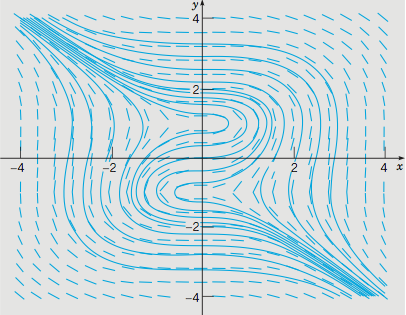
\includegraphics[scale=1]{L6directionfield2}
		\caption{Direction field for $\yp = \frac{x^2}{1 - y^2}$ with solutions.}
	\end{figure}
% end lecture 6 (21 September)

% start lecture 7 (26 September)
\section{Lecture 7 - Second Order ODEs}
\subsection{First order ODEs continued}
	\textbf{Theorem:} let the functions $f$ and $\frac{\partial f}{\partial y}$ be continuous in some rectangle $x \in (\alpha, \beta)$ and $y \in (\gamma, \delta)$ containing the point $(x_0, y_0)$. Then, in some interval $x \in (x_0 - h, x_0 + h)$ contained in $(\alpha, \beta)$, there is a unique solution $y = \varphi(x)$ to the initial value problem $\yp = f(x,y)$ with $y(x_0) = y_0$.

\subsection{General second order ODEs}
	The general second order nonlinear ODE has the form
		$$ \ypp = f(t, y, \yp) $$
	and there is no general solution technique for all such forms.

\subsection{Linear second order ODEs}
	The general form of a linear second order ODE is
		$$ a_0 (x) \sdx + a_1 (x) \fdx + a_2 (x) y = g(x) $$
	and if $g(x) = 0$, the ODE is homogeneous, otherwise it is non-homogeneous.

	If $a_0 (x), a_1 (x), a_2 (x)$ are all constant, we call this ODE \emph{constant-coefficient}, and we'll see below how to solve it. Otherwise, with variable coefficients, we will normally require series solutions to solve the ODE, which will be introduced later in the course.

\subsection{Linear homogeneous second order ODEs}
	The general form for linear homogeneous second order ODEs is
		$$ a_0 (x) \ypp + a_1 (x) \yp + a_2 (x) y = 0. $$

	Notice that if $y_1(x)$ and $y_2(x)$ are both functions which satisfy this ODE (i.e. $a_0 (x) y_1^{\prime\prime} + a_1 (x) y_1^{\prime} + a_2 (x) y_1 = 0$ and $a_0 (x) y_2^{\prime\prime} + a_1 (x) y_2^{\prime} + a_2 (x) y_2 = 0$), then, for any constants $c_1, c_2$, we have that
		$$ y(x) = c_1 y_1 (x)  + c_2 y_2 (x). $$
	Then,
		\begin{align*}
			a_0(x)\ypp + a_1(x)\yp + a_2(x) y &= a_0 (x) (c_1 \ypp_1 + c_2 \ypp_2) + a_1(x) (c_1 \yp_1 + c_2 \yp_2) + a_2(x) (c_1 y_1 + c_2 y_2) \\
				&= c_1 (a_0(x) \ypp_1 + a_1(x)\yp_1 + a_2(x) y_1) + c_2 (a_0(x) \ypp_2 + a_1(x)\yp_2 + a_2(x) y_2) \\
				&= 0.
		\end{align*}
	This equation evaluates to $0$ because each term in parentheses is $0$ as $y_1, y_2$ satisfy the ODE. Hence, $y$ itself is a solution to the ODE.

	\definition This is called the \emph{principle of superposition}, i.e. any linear combination of solutions is itself a solution.

	This principle suggests that the general solution to this ODE should be
		$$ y(x) = c_1 y_1 (x) + c_2 y_2 (x) $$
	where $y_1, y_2$ are ``different'' (linearly independent) solutions of the ODE.

\subsubsection{Linear Independence}
	\definition a set of functions $\{f_1(x), f_2 (x), \ldots, f_n (x)\}$  (excluding the trivial function $f_t(x) = 0$) is \emph{linearly dependent on an interval $I$} if there exists constants $c_1, c_2, \ldots, c_n$ (where not all are $0$) such that
		$$ c_1 f_1 (x) + c_2 f_2 (x) + \cdots + c_n f_n (x) = 0 $$
	for all $x \in I$. Otherwise, the set is said to be \emph{linearly independent on $I$}. At least two constants must be non-zero for the functions to be linearly dependent.

	Linear dependence is easy to check in the case where $n=2$, i.e. the functions $f_1(x), f_2(x)$ are linearly dependent if there exist constants $c_1, c_2 \neq 0$ such that
		$$ c_1 f_1(x) + c_2 f_2(x) = 0 $$
		$$ \frac{f_2(x)}{f_1 (x)} = - \frac{c_1}{c_2} = k $$
	where $k$ is constant. In other words, two functions are linearly dependent if and only if their ratio is a constant.

	We will seek to solve the homogeneous ODE to find the general solution
		$$ y(x) = c_1 y_1 (x) + c_2 y_2 (x) $$
	where $y_1, y_2$ are linearly independent.

\subsection{Linear homogeneous constant-coefficient second order ODEs}
	We'll find the general solution
		$$ y(x) = k_1 y_1 (x) + k_2 y_2 (x) $$
	to the ODE
		$$ a y'' + b y ' + cy = 0 $$
	where $a,b,c$ are constants.

	\example solve the IVP $y'' - k^2 y = 0$ where $k^2 > 0$ is constant, and $y(0) = 1, y'(0) = 0$. So far, we have no technique to solve this, so we'll have to guess. We're looking for a function which, when differentiated twice, looks like itself, e.g. $e^x, \sin(x), \cos(x)$. We'll guess $y = e^{rx}$ is a solution. Then,
		\begin{align*}
			y'' &= r^2 e^{rx} \\
			y'' - k^2 y &= 0 \\
			r^2 e^{rx} - k^2 e^{rx} &= 0 \\
			(r^2 - k^2) e^{rx} &= 0
		\end{align*}
	Since $e^{rx} \neq 0$, for $e^{rx}$ to be a solution, we'll need that $r^2 - k^2 = 0$ i.e. $r = \pm k$.

	Hence, both $e^{rx}$ and $e^{-rx}$ are solutions to the ODE, and the general solution is $y_1 = e^{kx}$ and $y_2 = e^{-kx}$, so
		$$ y(x) = c_1 e^{kx} + c_2 e^{-kx} $$
	Notice that $y_1$ and $y_2$ are linearly independent.

	To satisfy the initial conditions $y(0) = 1, y'(0) = 0$, take $y(x) = c_1 e^{kx} + c_2 e^{-kx}$ and evaluate at $x = 0$. Then, $1 = c_1 + c_2$, and differentiating $y(x)$ to find
		$$ y'(x) = c_1 k e^{kx} - c_2 k e^{-kx} $$
	We'll find that $c_1 = c_2 = \frac{1}{2}$, so our IVP's solution is
		$$ y(x) = \frac{1}{2} e^{kx} + \frac{1}{2} e^{-kx} $$

	Notice that to solve the IVP, we specify $y(x_0)$ and $y'(x_0)$, which for the general ODE is the minimum information needed just to evaluate $y''(x_0)$, and it turns out that this is sufficient to specify a unique solution of the IVP.

\subsubsection{Theory}
	To solve $a y'' + b y' + c y = 0$, let $y(x) = e^{rx} \Rightarrow y'(x) = r e^{rx} \Rightarrow y''(x) r^2 e^{rx}$. If $y(x)$ is a solution, then
		$$ 0 = ay'' + by' + cy = a r^2 e^{rx} + b r e^{rx} + c e^{rx} $$
		$$ \Rightarrow 0 = (a r^2 + b r + c) e^{rx} $$
	We know $e^{rx} \neq 0$, so
		$$ a r^2 + b r + c = 0 $$
	Therefore, to deal with the ODE, we will have to solve this quadratic equation. This equation is called the \emph{Auxiliary Equation} or the \emph{Characteristic Equation}. There are three cases to consider:
		\begin{enumerate}
			\item $b^2 > 4ac$
			\item $b^2 = 4ac$
			\item $b^2 < 4ac$
		\end{enumerate}
	\textbf{Case 1:} for the first case, there are two distinct real roots $r \neq s$. Since
		$$ \frac{e^{rx}}{e^{sx}} = e^{(r-s)x} $$
	which is not constant when $r \neq s$. In this case, $y_1 (x) = e^{rx}$ and $y_2 (x) = e^{sx}$ are linearly independent and the general solution is
		$$ y(x) = k_1 e^{rx} + k_2 e^{sx} $$

	\textbf{Case 2:} with the second case, there is a single repeated root $r$ (i.e. $r = s$). $y_1(x) = e^{rx}$ is a solution, but to get $y_2(x)$, we'll need to use Reduction of Order.

\subsubsection{Reduction of Order}
	The idea of reduction of order is as follows: given a solution $y_1 (x)$, we let $y(x) = u(x) y_1 (x)$, where we assume $y(x)$ is another solution of the ODE and $u(x)$ is an unknown solution we will find.
		$$ y'(x) = u'(x) y_1 (x) + u (x) \yp_1 (x) $$
		$$ y''(x) = u''(x) = y_1(x) + 2 u'(x) \yp_1 (x) + u(x)\ypp_1(x) $$
	So if $y(x)$ is a solution of the ODE, then
		\begin{align*}
			0 &= ay'' + by' + cy \\
				&= a(u'' y_1 + 2 u' \yp_1 + u \ypp_1) + b(u' y_1 + u \yp_1) + c (u y_1) \\
				&= u(a\ypp_1 + b\yp_1 + c y_1) + u'(2a\yp_1 + by_1) + u'' a y_1
		\end{align*}
	We know that, since $y_1$ was a solution, then $a\ypp_1 + b\yp_1 + c y_1 = 0$, so:
		$$ \Rightarrow (ay_1) u'' + (2a\yp_1 + by_1) u' $$
	Letting $v = u'$, we can transform this into a first order linear homogeneous ODE:
		$$ \Rightarrow 0 = (ay') v' + (2a\yp_1 + by_1) v $$
	and we can solve this as any other ODE of the same type by finding the integrating factor. After solving this ODE (finding $v$), we can find $u$ by solving the equation $v = u'$. Then, finally, $y = u y_1$ is another solution of the second order ODE.

\subsubsection{Theory continued}
	\textbf{Case 2 continued:} recall that, in the case where $a y'' +  by' + c = 0$ with $b^2 = 4ac$, the characteristic equation has a single root $r$ where $r = \frac{-b}{2a}$ and $y_1(x) = e^{r x}$ is a solution.
		$$ y(x) = u(x)y_1(x) = u e^{r x} $$
		$$ y' = u' e^{rx} + u r e^{rx} $$
		$$ y'' = u'' e^{rx} + 2 u' r e^{rx} + u r^2 e^{rx} $$
	Then,
		\begin{align*}
			0 &= ay'' + by' + cy \\
				&= a(u'' e^{rx} + 2 u' r e^{rx} + u r^2 e^{rx}) + b (u' e^{rx} + u r e^{rx}) + c (u e^{rx}) \\
				&= e^{rx}(u (ar^2 + b r + c) + u' (2ar + b) + u'' a)
		\end{align*}
	We know that $a r^2 + b r + c = 0$ since $r$ solves the quadratic, and $2 a r + b = 0$ as $r = \frac{-b}{2a}$, hence
		$$ \Rightarrow 0 = a e^{rx} u'' $$
	but $a \neq 0$ (since this is a second order ODE) and $e^{rx} \neq 0$, so $u'' = 0$. Then, $u' = k$ and $u = k_1x + k_2$.

	Thus, $y(x) = u(x) y_1 (x) = (k_1 x + k_2) e^{rx}$ must solve the ODE. $y_1 (x) = e^{rx}$ already solves the ODE, so we'll rewrite this as
		$$ y(x) = k_1 x e^{rx} + k_2 e^{rx} $$
	so let $k_1 = 1$ and $k_2 = 0$ and let $y_2 (x) = x e^{rx}$ which is a solution of the ODE since $y_1$ and $y_2$ are linearly independent (as $\frac{y_2}{y_1} = x$ is not constant).
% end lecture 7 (26 September)

% start lecture 8 (28 September)
\section{Lecture 8 - More second order ODEs}
\subsection{Linear homogeneous constant-coefficient second order ODEs continued}
\subsubsection{Theory (roots of the characteristic equation) continued}
	\textbf{Case 3:} In the case where $b^2 < 4ac$, there are zero real roots and two complex roots to the characteristic equation $a r^2 + b r + c = 0$. The roots, $r$ and $s$ are
		$$ r = \alpha + i \beta \text{ and } s = \alpha - i \beta $$
	In this case, $y_1 (x) = e^r = e^{\alpha + i \beta}$ and $y_2 (x) = e^s = e^{\alpha - i \beta}$ are both complex solutions to the ODE.

	We'll use the \emph{principle of superposition} to find the real solutions. First, recall Euler's Formula:
		$$ e^{i\theta} = \cos(\theta) + i \sin(\theta) $$
	and recall the series expansion of $e^x$:
		$$ e^x = 1 + x + \frac{x^2}{2} + \frac{x^3}{3!} + \ldots $$
	Now, with the fact that $i^2 = -1$:
		$$ e^{i \theta} = 1 + i \theta - \frac{\theta^2}{2} - \frac{i\theta^3}{3!} + \frac{\theta^4}{4!} + \ldots $$
		$$ cos(\theta) = 1 - \frac{\theta^2}{2} + \frac{\theta^4}{4!} - \ldots $$
		$$ sin(\theta) = \theta - \frac{\theta^3}{3!} + \frac{\theta^5}{5!} - \ldots $$
	Using these facts:
		$$ y_{+}(x) = e^{\alpha x} e^{i \beta x} = e^{\alpha x}(\cos(\beta x) + i \sin(\beta x)) $$
		$$ y_{-}(x) = e^{\alpha x} e^{-i\beta x} = e^{\alpha x}(\cos(-\beta x) + i \sin(- \beta x)) $$
	Recall that $\cos(\beta x) = \cos(- \beta x)$ and $\sin(-\beta x) = - \sin(\beta x)$. Thus,
		$$ y_{-}(x) = e^{\alpha x} (\cos(\beta x) - i \sin(\beta x)) $$
	Comparing these solutions, we see that
		\begin{align*}
			y_1 (x) &= \frac{1}{2} y_{+} (x) + \frac{1}{2} y_{-} (x) \\
				&= e^{\alpha x} \cos(\beta x)
		\end{align*}
	Here, $y_1(x)$ is real and solves the ODE. To find the second solution, subtract
		$$ y_{+} - y_{-}(x) = 2ie^{\alpha x} \sin(\beta x) $$
	This is imaginary, but
		$$ y_2 (x) = \frac{1}{2i} (y_{+} (x) - y_{-}(x)) = e^{\alpha x} \sin(\beta x) $$
	gives us the second real solution.

	Now, when $b^2 < 4ac$ in the characteristic equation, the general solution is
		$$ y(x) = e^{\alpha x} (k_1 \cos(\beta x) + k_2 \sin(\beta x)) $$
	where $r = \alpha \pm i \beta$ are the complex roots.

	Notice that the real solutions $y_1, y_2$ are just the real and imaginary parts of the complex solutions.

\subsubsection{Summary for these ODEs}
	Given $a y'' + b y' + c = 0$ where $a,b,c$ are constant, the auxiliary equation $ar^2 + br + c = 0$ has three possible cases:
		\begin{enumerate}
			\item $b^2 > 4ac$ -- distinct roots $r \neq s$, general solution $y(x) = k_1 e^{rx} + k_2 e^{s x}$.
			\item $b^2 = 4ac$ -- single repeated root $r = \frac{-b}{2a}$, general solution $y(x) = (k_1 x + k_2) e^{rx}$.
			\item $b^2 < 4ac$ -- complex roots $r = \alpha \pm i \beta$, general solution $y(x) = e^{\alpha x} (k_1 \cos(\beta x) + k_2 \sin (\beta x))$.
		\end{enumerate}

\subsubsection{Examples}
	\example $y'' - 3y' + 2y = 0$. Let $y = e^{rx} \Rightarrow r^2 e^{rx} - 3re^{rx} + 2 e^{rx} = 0$. So $e^{rx} (r^2 - 3r + 2) = 0$. $e^{rx} \neq 0$ so
		\begin{align*}
			r^2 - 3r + 2 &= 0 \\
			(r-1)(r-2) &= 0
		\end{align*}
	$r = 1$ and $s = 2$, so this follows the first case, and the general solution is
		$$ y(x) = k_1 e^x + k_2 e^{2x} $$

	\example $y'' - 2y' + y = 0$. Aux: $r^2 - 2r + 1 = 0$, repeated root $r = 1$. Case 2: general solution:
		$$ y(x) = (k_1 x + k_2) e^x $$

	\example $y'' + 4y' + 7y = 0$. Aux $r^2 + 4r + 7 = 0$.
		$$ r = \frac{-4 \pm sqrt{4^2 - (4)(1)(7)}}{2} = -2 \pm i \sqrt{3} $$

	General solution:
		$$ y(x) = e^{-2x} (k_1 \cos(\sqrt{3} x) + k_2 \sin(\sqrt{3} x)) $$
	Don't forget the minus sign if $\alpha < 0$, and $\beta$ is always positive.

\subsection{Variable-coefficient second order homogeneous ODEs}
	General form:
		$$ a_0(x) y'' + a_1 (x) y' + a_2 (x) y = 0 $$
	There is no general solution technique for these ODEs. Later on in the course, we'll be able to use series solutions to solve these. If we can find one solution (e.g. by inspection), we can find a second using reduction of order.

	There is one important special class of these ODEs which we can solve called \emph{Euler Equations} (a.k.a. Cauchy-Euler, Euler-Cauchy, or Equidimensional equations).

\subsubsection{Euler Equations}
	General form (with $a,b,c$ constant):
		$$ ax^2 y'' + b x y' + c y = 0 $$
	To solve, guess $y = x^r$:
		$$ y = x^r \Rightarrow y' = rx^{r-1} \Rightarrow r(r-1)x^{r-2} $$
	So, if $y = x^r$ is a solution,
		\begin{align*}
			0 &= ax^2y'' + bxy' + cy \\
				&= ax^2 r (r-1) x^{r-2} + b x r x^{r-1} + c x^r \\
				&= x^r (a r(r-1) + br + c)
		\end{align*}
	Hence $y = x^r$ is a solution if $r$ satisfies the \emph{indicial equation}
		$$ a r^2 + (b-a) r + c = 0 $$

	\textbf{Remarks:} $r$ is a root of the quadratic, so it may be real or complex, thus $x^r$ can be problematic if $x < 0$ or $x = 0$. For now, only consider the cases where $x > 0$. Again, there are three cases to consider, where the indicial equation $a r^2 + (b-a) r + c = 0$ has...
		\begin{enumerate}
			\item ... distinct real roots $r,s$. The general solution would be $y(x) = k_1 x^r + k_2 x^s$ for $x > 0$.
			\item ... one repeated root $r = \frac{-(b-a)}{2a}$. We have one solution $y_1 = x^r$ for $x > 0$. Use reduction of order to find the other solution.
			\item ... complex roots $r = \alpha \pm i \beta$.
		\end{enumerate}

\subsubsection{Reduction of order (for case 2)}
	Let $y = u y_1 = u x^r$, $y' = u' y_1 + u \yp_1$, and $y'' = u'' y_1 + 2 u' \yp_1 + u \ypp_1$.

	\begin{align*}
		0 &= ax^2 y'' + b x y' + cy \\
			&= a x^2 (u'' y_2 + 2u' \yp_1 + u \ypp_1) + bx(u' y_1 + u \yp_1) + cu(y_1) \\
			&= u (ax^2y'' + bxy' + cy_1) + u' (2ax^2 \yp_1 + bxy_1) + ax^2 y_1 u'' \\
			&= u (0) + u' (2ax^2 \yp_1 + bxy_1) + ax^2 y_1 u'' \\
			&= u' (2ax^2 \yp_1 + bxy_1) + ax^2 y_1 u'' \\
	\end{align*}

	$y_1 = x^r \Rightarrow y' = r x^{r-1} $
	\begin{align*}
		2ax^2 \yp_1 + bxy_1 &= 2ax^2rx^{r-1} + bx^r \\
			&= (2ar + b)x^r
	\end{align*}

	But $r = \frac{-(b-a)}{2a} \Rightarrow 2ar + b = a$.
	\begin{align*}
		0 &= x^{r+1} a u' + a x^2 x^r u'' \\
			&= ax^{r+1} (x u'' + u')
	\end{align*}
	So $0 = xu'' + u'$. Let $v = u' \Rightarrow 0 = xv' + v \Rightarrow 0 = \frac{d}{dx} (xv)$, so $xv = k$ with $k$ constant. $u' = v = \frac{k}{x}$, so $u = k_1 \ln(x) + k_2$. Our general solution is
		$$ y = u y_1 = (k_1 \ln(x) + k_2) x^r $$
	for $x > 0$.

\subsubsection{Euler equations continued}
	\textbf{Case 2:} the general solution for $x > 0$ is
		$$ y(x) = (k_1 \ln(x) + k_2) x^r $$

	\textbf{Case 3:} the indicial equation $ar^2 + (b-a) r + c = 0$ has roots $r = \alpha + i \beta$. We have the complex solutions
		$$ y_1 (x) = x^{\alpha + i \beta} = x^{\alpha} x^{i \beta} = x^{\alpha}(e^{\ln(x)})^{i \beta} = x^{\alpha}e^{i \beta \ln(x)} $$

	Using Euler's formula:
		$$ x^{\alpha} e^{i \beta \ln(x)} = x^{\alpha} (\cos(\beta \ln(x)) + i \sin(\beta \ln(x))) $$
	Similarly,
		$$ y_2 (x) = x^{\alpha - i \beta} \Rightarrow y_2 (x) = x^{\alpha} (\cos(\beta \ln(x)) - i \sin(\beta \ln(x))) $$
	As before, the real and imaginary parts both define solutions by taking the linear combinations of them. Therefore, the general solution for $x > 0$ is
		$$ y(x) = x^{\alpha} (k_1 \cos(\beta \ln(x)) + k_2 \sin (\beta \ln(x))) $$

	\textbf{When $x < 0$:} make a change in variables. Let $\xi = -x$ when $x < 0$, so $\xi > 0$. Then,
		$$ \frac{dy}{d\xi} = \frac{dx}{d\xi} \frac{dy}{dx} = - \fdx $$
		$$ \frac{d^2y}{d\xi^2} = \sdx $$
	Then,
		$$ 0 = ax^2\sdx + bx\fdx + cy $$
		$$ \Rightarrow 0 = a \xi^2 \frac{d^2 y}{d\xi^2} + (-\xi)(- \frac{dy}{d\xi}) + cy = 0 $$
	Noting that $b (-\xi) (- \frac{dy}{d\xi}) = b \xi \frac{dy}{d\xi}$, we can see that this is the same ODE. When $x < 0$, this ODE has $\xi = -x > 0$, so we can solve as before.

	Notice for the first ODE, $|x| = x$ since $x > 0$, and for the second ODE, $\xi = -x = |x|$ since $x < 0$. So if we replace $x$ by $|x|$ above, the solutions are valid for all $x \neq 0$.
% end lecture 8 (28 September)

% start lecture 9 (03 October)
\section{Lecture 9 - More on Euler equations, some theory, and Wronskian equations}
\subsection{Euler Equations continued}
\subsubsection{Summary}
	General form:
		$$ a x^2 y'' + b x y' + c y = 0 $$
	Indicial equation:
		$$ a r^2 + (b-a) r + c = 0 $$
	Three possible situations (all for $x \neq 0$):
		\begin{enumerate}
			\item distinct real roots $r \neq s$, general solution: $y(x) = k_1 |x|^r + k_2 |x|^s$.
			\item repeated root $r$, general solution: $y(x) = (k_1 + k_2 \ln(|x|) |x|^r$.
			\item complex roots $r = \alpha \pm i \beta$, general solution: $y(x) = |x|^{\alpha} (k_1 \cos(\beta \ln(|x|)) + k_2 \sin(\beta \ln(|x|)))$.
		\end{enumerate}
	If we consider solutions just for $x > 0$, we can omit the absolute signs.

\subsubsection{Examples}
	\example solve $x^2 y'' - 2 x y' - 4y = 0$ for $x > 0$. If we forget the indicial equation, we can easily derive it again. Let $y = x^r$, $\Rightarrow x^r (r (r - 1) - 2r - 4) = 0$. $r^2 - 3r - 4 = 0$ $\Rightarrow (r - 4)(r + 1) = 0$, so $r = 4$ and $s = -1$. Our general solution is therefore $y(x) = k_1 x^4 + k_2 x^{-1}$ for $x>0$ (but this is also valid $\forall x \neq 0$).

	\example solve $4x^2 y'' + 8xy' + y = 0$ for $x \neq 0$. Our indicial equation is $4 r^2 + 4r + 1 = 0 \Rightarrow (2r + 1)^2 = 0$, so $r = - \frac{1}{2}$ is a repeated root. Therefore, our general solution $\forall x \neq 0$ is
		$$ y(x) = (k_1 + k_2 \ln(|x|))|x|^{-\frac{1}{2}} $$

	\example solve $4xy'' + 17y + 0$ with $y(1) = -1$ and $y'(1) = -\frac{1}{2}$. This is a Euler equation with coefficient $b = 0$. Therefore, our same theory as above applies. Since the initial conditions pose at $x = 1$, we'll solve for $x > 0$.

	Our indicial equation is $4 r^2 - 4r + 17 = 0$, so
		$$ r = \frac{-(-4) \pm \sqrt{(-4)^4 - (4)(4)(17)}}{(2)(4)} = \frac{1}{2} \pm 2 i $$
	Our general solution is now
		$$ y(x) = x^{\frac{1}{2}} (k_1 \cos(2 \ln x) + k_2 \sin(2 \ln x)) $$
	for $x > 0$. Now use the initial conditions to find constants $k_1, k_2$. First, $-1 = y(1) = k_1$. We have $y'(1) = -\frac{1}{2}$, so find $y'(x)$:
		$$ y'(x) = \frac{1}{2} x^{-\frac{1}{2}} (k_1 \cos(2 \ln x) + k_2 \sin(2 \ln x)) + x^{\frac{1}{2}}(-2 \frac{k_1}{x} \sin(2 \ln x) + 2 \frac{k_2}{x} \cos(2 \ln x)) $$
	Now, $\frac{-1}{2} = y'(1) = \frac{1}{2} k_1 + 2 k_2 \Rightarrow k_2 = 0$. Therefore, the solution of the IVP is
		$$ y(x) = - x^{\frac{1}{2}} \cos(2 \ln x) $$
	for $x > 0$.

\subsection{Theory for second and higher order homogeneous ODEs}
	\definition $\{y_1 (x), \ldots, y_n (x)\}$ are called a \emph{fundamental set of solutions} on an interval $I \subseteq \mathbb{R}$ for the $n$th order linear homogeneous ODE
		$$ y^{(n)}(x) + p_1 (x) y^{(n-1)} (x) + p_2 (x) y^{(n-2)} (x) + \ldots + p_n (x) y (x) = 0 $$
	or
		$$ y^{(n)}(x) + \sum_{j = 0}^{n-1} p_{n-j}(x) y^{(j)} (x) = 0 $$
	if each $y_i(x)$ is a (non-trivial) solution of the ODE and, moreover, $y_1, \ldots, y_n$ are linearly independent on $I$. In that case, the general solution of the ODE is:
		$$ y(x) = \sum_{i = 1}^n k_i y_i (x). $$
	Note that a non-trivial solution $y(x)$ is simply a solution that is not everywhere zero.

	Recall that $y_1, \ldots, y_n$ are linearly dependent on an interval $I$ if there exists constants $k_i$ not all zero such that
		$$ \sum_{i=1}^n k_i y_i (x) = 0 $$
	$\forall x \in I$. Otherwise, the functions are considered linearly independent on $I$.

	In the case of two functions $y_1$ and $y_2$, we saw that they are linearly dependent if and only if
		$$ \frac{y_1 (x)}{y_2 (x)} = \frac{-k_2}{k_1} $$
	is constant for all values of $x \in I$.

	\textbf{What about three or more functions?}

	\example let $f_1 (x) = 1 + 2x$, $f_2 (x) = 2 + x^2$, and $f_3 (x) = 2x^2 - 8x$. Note that $\frac{f_i(x)}{f_j(x)}$ is not constant for any $i \neq j$, but $2 f_1 (x) - f_2 (x) + \frac{1}{2} f_3 9x) = 0$ for all values of $x \in I$, so these functions are linearly dependent.

	Say we are given functions $1, x, x^2$ -- how can we determine if they are linearly dependent or independent? This can be done from first principles, but it is tedious. We'll first find out this way, then we'll find a shortcut for the future.

	\example show $1, x, x^2$ are linearly independent on $\mathbb{R}$. To ``prove'' this by contradiction, assume that they are linearly dependent, i.e.
		$$ k_1 + k_2 x + k_3 x^2 = 0 \; \forall x \in \mathbb{R} $$
	So this must be true for $x = 0$:
		$$ \Rightarrow k_1 + 0 + 0 = 0 \Rightarrow k_1 = 0 $$
	and also for $x = 1$:
		$$ \Rightarrow k_1 + k_2 + k_3 = 0 \Rightarrow k_2 + k_3 = 0 \Rightarrow k_2 = - k_3$$
	and also for $x = -1$:
		$$ \Rightarrow k_1 - k_2 + k_3 = 0 \Rightarrow k_2 = k_3. $$
	Because $k_2 = k_3$ and $k_2 = - k_3$, the only possible value for $k_2$ and $k_3$ is zero, so $k_1 = k_2 = k_3 = 0$. However, we assumed that the three functions were linearly dependent, so the values of all three constants cannot be zero, therefore these functions must be linearly independent.

	This process is tedious for even three simple functions, so we need to find a shortcut.

\subsubsection{The Wronskian equation}
	\definition The Wronskian $W(y_1, y_2, \ldots, y_n)(x)$ of $n$ functions $y_1, y_2, \ldots, y_n$ is defined to be
		$$ W(y_1, y_2, \ldots, y_n)(x) = \left|
			\begin{array}{cccc}
				y_1 (x) & y_2 (x) & \ldots & y_n (x) \\
				\yp_1 (x) & \yp_2 (x) & \ldots & \yp_n (x) \\
				\ypp_1 (x) & \ypp_2 (x) & \ldots & \ypp_n (x) \\
				\vdots & \vdots & \ldots & \vdots \\
				y_1^{(n-1)} (x) & y_2^{(n-1)}(x) & \ldots & y_n^{(n-1)} (x)
			\end{array} \right|. $$
	So the Wronskian equation for $n$ functions is defined to be the determinant of an $n \times n$ matrix where the matrix entries are all functions of $x$.

	In the case of two functions:
		$$ W (y_1, y_2) (x) = \left|
			\begin{array}{cc}
				y_1(x) & y_2 (x) \\
				\yp_1 (x) & \yp_2 (x)
			\end{array} \right| = y_1(x) \yp_2(x) - \yp_1(x) y_2(x) $$

	Notice that if $y_1, y_2$ are linearly dependent, then, for $k_1, k_2 \neq 0 \; \forall x \in I$:
		$$ k_1 y_1(x) + k_2 y_2 (x) = 0 \Rightarrow k_1 \yp_1 (x) + k_2 \yp_2 (x) = 0. $$
	Now, by the first (undifferentiated) equation, $k_1 y_1 (x) \yp_2 (x) = 0 \text{ and } k_2 y_2 (x) \yp_2 (x) = 0$, and by the second (differentiated) equation, $k_1 \yp_1 (x) y_2 (x) + k_2 y_2(x) \yp_2 (x) = 0$. So now
		$$ W(y_1, y_2) (x) = y_1 (x) \yp_2 (x) - y_2 (x) \yp_1 (x) $$
		$$ \Rightarrow W(y_1, y_2) (x) = \frac{-k_2}{k_1} y_2 (x) \yp_2 (x) + \frac{k_2}{k_1} y_2 (x) \yp_2 (x) = 0 $$
	So if $y_1, y_2$ are linearly dependent on an interval $I$, then $W(y_1, y_2) (x) = 0$ for all values of $x \in I$.

	\example let $y_1 = 1, y_2 = x, y_3 = x^2$. Now,
		$$ W(y_1, y_2, y_3)(x) =
			\left|
				\begin{array}{ccc}
					y_1 (x) & y_2 (x) & y_3 (x) \\
					y'_1 (x) & y'_2 (x) & y'_3 (x) \\
					y''_1 (x) & y''_2 (x) & y''_3 (x)
				\end{array}
			\right| =
			\left|
				\begin{array}{ccc}
					1 & x & x^2 \\
					0 & 1 & 2x \\
					0 & 0 & 2
				\end{array}
			\right|
		$$
		Recall from linear algebra that the determinant of a triangular matrix is the product of the terms on the diagonal. Therefore, $W(y_1, y_2, y_3)(x) = 2$, but we saw earlier that these functions $y_1 = 1, y_2 = x, y_3 = x^2$ are linearly independent, and we suspect that $W(y_1, \ldots, y_n)(x) = 0$ for linearly dependent functions $y_1, \ldots, y_n$ and $W(y_1, \ldots, y_n)(x) \neq 0$ for linearly independent functions. This is not quite true, however.

	\example $y_1 (x) = x^2, y_2 = \left\{ \begin{array}{ccc} x^2 & \text{ for } & x \geq 0 \\ - x^2 & \text{ for } & x < 0 \end{array} \right. $. Note that both $y_1$ and $y_2$ are continuously differentiable on $\mathbb{R}$, so we can compute the Wronskian for all values of $x$.
		$$ W(y_1,  y_2)(x) =
			\left\{
				\begin{array}{ccc}
					\left|
						\begin{array}{cc}
							x^2 & x^2 \\
							2x & 2x
						\end{array}
					\right| = 0 & \text{ for } & x \geq 0 \\
					\left|
						\begin{array}{cc}
							x^2 & -x^2 \\
							2x & -2x
						\end{array}
					\right| = 0 & \text{ for } & x < 0
				\end{array}
			\right.
		$$

	So we can see that $W(y_1, y_2)(x) = 0$ for all $x \in \mathbb{R}$, but are $y_1, y_2$ linearly dependent on $\mathbb{R}$?
		$$ k_1 y_1 (x) + k_2 y_2 (x) = 0 $$
	Our only solution to this is $k_1 = k_2 = 0$, so $y_1$ and $y_2$ are linearly independent on $\mathbb{R}$. However, on $(0, \infty)$ and $(-\infty,0)$, they are linearly dependent.

	\textbf{Theorem:} let $y_1, \ldots, y_n$ be $(n-1)$-times continuously differentiable on an interval $I$. If the Wronskian $W(y_1,\ldots,y_n)(x) \neq 0$ for some point $x_0 \in I$, then the functions are linearly independent on $I$.

	\textbf{Remark:} this theorem tells us nothing about the case where the Wronskian equals $0$ for all values of $x \in I$. In that case, we have already seen examples with the Wronskian equaling $0$ with the functions either linearly independent or linearly dependent.
% end lecture 9 (03 October)

% start lecture 10 (05 October)
\section{Lecture 10 - The Wronskian continued, Abel's Formula, and Higher-Order ODEs}
\subsection{Differential Operators}
	Once we get into $n$th order ODEs, we'll get tired of writing
		$$ y^{(n)} (x) + p_1 (x) y^{(n-1)} (x)  + p_2 (x) y^{(n-2)} (x) + \ldots + p_{n-1}(x) y' (x) + p_n (x) y $$
	so we'll introduce a more compact notation using \emph{differential operators}.

	Let $D$ be the differential operator such that
		$$ D y = D [y] := \fdx = y'. $$
	We notice that $D$ is a linear operator, so $D[\alpha y] = \alpha D[y]$ for all constant $\alpha$, and $D[y_1 + y_2] = D[y_1] + D[y_2]$, as evidenced by the standard rules of derivatives.

	Now, let $L$ be the more complicated differential operator
		$$ L = D^n + \sum_{j = 0}^{n-1} p_{n-j} (x) D^j $$
	where $D = D[y] = y', D^2 = D[D[y]] = y'', \ldots$. Thus,
		$$ L[y] = [D^n + \sum_{j = 0}^{n-1} p_{n-j} (x) D^j] y = y^{(n)} + \sum_{j = 0}^{n - 1} p_{n-j}(x) y^{(j)} $$
	and
		$$ y^{(n)} + \sum_{j = 0}^{n - 1} p_{n-j}(x) y^{(j)} =  y^{(n)} (x) + p_1 (x) y^{(n-1)} (x)  + p_2 (x) y^{(n-2)} (x) + \ldots + p_{n-1}(x) y' (x) + p_n (x) y. $$
	Thus, $L[y] = y^{(n)} (x) + p_1 (x) y^{(n-1)} (x)  + p_2 (x) y^{(n-2)} (x) + \ldots + p_{n-1}(x) y' (x) + p_n (x) y$, so we can write our homogeneous ODE in shorthand notation as
		$$ L[y] = 0 $$
	and the non-homogeneous version as
		$$ L[y] = g(x). $$

\subsection{The Wronskian and Abel's Theorem}
\subsubsection{Abel's Theorem}
	\textbf{Theorem:} let $I$ by an interval on the real line and $x_0 \in I$. Let $p_i (x)$ and $g(x)$ be continuous on $I$. Then, the IVP $L[y] = g(x)$ with $y(x_0) = c_1, y'(x_0) = c_2, \ldots, y^{(n-1)} (x_0) = c_n$ has a unique solution $y(x)$ which exists and is $n$-times continuously differentiable on $I$.

	\textbf{Theorem:} let $y_1, \ldots, y_n$ be solutions on $I$ of the $n$th order homogeneous ODE $L[y] = 0$. Then, the Wronskian $W(y_1, \ldots, y_n)(x)$ (which we write as $W(x)$) satisfies the ODE
		$$ W' + p_1(x) W = 0 $$
	and hence
		$$ W(x) = ce^{- \int p_1(x)\dx}. $$
	Now, either $W(x) \neq 0$ for all values of $x \in I$ and $y_1, \ldots, y_n$ are a fundamental set of solutions, or $W(x) = 0$ for all $x \in I$ meaning $y_1, \ldots, y_n$ are linearly dependent.

	\textbf{Notes:} hence if $W(x) = 0$ $\forall x \in I$ but $y_1, \ldots, y_n$ are linearly independent, then there \emph{does not} exist an $n$th order linearly homogeneous ODE for which $y_1, \ldots, y_n$ are all solutions on $I$.

	For example, for $y_1 (x) = x^2, y_2 = \left\{ \begin{array}{ccc} x^2 & \text{ for } & x \geq 0 \\ - x^2 & \text{ for } & x < 0 \end{array} \right. $, there is no second order ODE which has these solutions on $I = [-1,1]$.

	The result that $W' + p_1 (x) W = 0$ and that $W(x) = ce^{- \int p_1(x)\dx}$ are often called \textbf{Abel's Theorem}, or Abel's Formula, or Abel's Identity. We will derive this formula for the case of second order ODEs, and it's simple to extend it to $n$th order ODEs.

\subsubsection{Deriving Abel's Theorem}
	Suppose $y_1$ and $y_2$ solve the ODE
		$$ y'' + p_1 (x) y' + p_2(x) y = 0. $$
	Then,
		$$ -y_2 [y'' + p_1 (x) y' + p_2(x) y] = 0 $$
	and
		$$ y_1 [y'' + p_1 (x) y' + p_2(x) y] = 0. $$
	Adding these together:
		$$ (y' y''_2 - y_2 y''_1) + p_1 (x) (y_1 y'_2 - y_2 y'_1) = 0 $$
	Notice that
		$$ W(x) = \left| \begin{array}{cc} y_1 & y_2 \\ y'_1 & y'_2 \end{array} \right| = y_1 y'_2 - y_2 y'_1 $$
	and
		$$ W'(x) = y_1 y''_2 - y_2 y''_1. $$

	We have shown that $W(x)$ satisfies the ODE $W' + p_1 (x) W = 0$.

\subsubsection{Finding the Wronskian for an IVP without actually solving the IVP}
	It is possible to find $W(x)$ as a function of $x$ for an IVP \emph{without} solving the IVP. We can use Abel's Formula to do so.

	\example suppose we have an ODE
		$$ 2x^2 y'' + 3x y' - y = 0 $$
	and let $y_1, y_2$ be two solutions of the IVP with $y_1 (1) = 1, y'_1 (1) = \frac{1}{2}, y_2 (1) = 1, y'_2 (1) = -1$. Given this information, we can evaluate the Wronskian at the given $x$ value, i.e. $W(y_1, y_2)(1)$:
		$$ W(y_1, y_2)(1) =
			\left|
				\begin{array}{cc}
					1 & 1 \\
					\frac{1}{2} & -1
				\end{array}
			\right| = -1 - \frac{1}{2} = - \frac{3}{2}.
		$$
	Since $W(x) \neq 0$ for a value of $x$ on $I = \mathbb{R}$, we know that $y_1, y_2$ are linearly independent. Now we can use Abel's Formula to calculate $W(y_1, y_2)(x)$.
		$$ W(y_1, y_2)(x) = c e^{- \int p(x)\dx} $$
	Here, $p_1 (x) = \frac{3x}{2x^2} = \frac{3}{2} x$, as the definition of $L[y]$ has $y^{(n)}$ not multiplied by any thing, so we'll have to divide every $p_i(x)$ by $2x^2$ to gain the ``true'' value of $p_i(x)$.
		$$ W(x) = c e^{-\int \frac{3}{2x}} = c x^{- 3/2} $$
	but now
		$$ -\frac{3}{2} = W(y_1, y_2) (1) = c (1)^{- 3 / 2} = c $$
	so
		$$ W(y_1, y_2)(x) = -\frac{3}{2} x^{-3/2}. $$
	Notice that $W(y_1, y_2)(x) > 0$ for all $x > 0$, but $W(y_1, y_2)(0) = 0$, so by the previous theorem, the solutions $y_1, y_2$ are not valid at $x = 0$, and the longest interval for which we can solve the IVP is $(0, \infty)$.

\subsubsection{Finding the fundamental set of solutions using Abel's Formula}
	For variable-coefficient ODEs. we can sometimes use Abel's Theorem to find a fundamental set of solutions.

	\example consider the ODE
		$$ L[y] = y'' - \frac{x + 2}{x} y' + \frac{x + 2}{x^2} y = 0 $$
	which is not a constant-coefficient equation, nor a Euler equation.

	However, notice that if $y = x$, then $y' = 1$ and $y'' = 0$. So then
		$$ L[y] = L[x] = 0 - \frac{x+2}{x} (1) + \frac{x+2}{x^2} x = 0 $$
	so $L[y] = 0$ if $y = x$, therefore $y = x$ is a solution.

	To find a second solution, we will use Abel's Formula. To find the Wronskian:
		$$ W' + p_1 W = 0 \Rightarrow W' - \frac{x + 2}{x} W = 0 $$
	so
		$$ W(x) = c e^{- \int - \frac{x + 2}{x}} = \ldots = c x^2 e^x. $$
	Now to find a second a solution $y_2 (x)$, given that $y_1(x) = x$ is one solution, use the definition of the Wronskian, i.e.
		$$ c x^2 e^x = W(y_1, y_2)(x) = y_1 (x) y'_2 (x) - y_2 (x) y'_1(x) $$
	with $y_1(x) = x$ and $y'_1(x) = 1$. Then,
		$$ c x^2 e^x = x y'_2 - y_2 $$
	or
		$$ y'_2 - \frac{1}{x} y_2 = cxe^x $$
	which is a linear first order ODE. Find the integrating factor as usual:
		$$ \mu = e^{- \int \frac{1}{x}\dx} = x^{-1} $$
	so
		\begin{align*}
			(x^{-1} y_2)' &= x^{-1}y' - x^{-2}y)2 = ce^x \\
			x^{-1} y_2 &= k_1 + \int c e^x \dx \\
				&= k_1 + c e^x \\
			y_2 &= k_1 x + c x e^x
		\end{align*}
	but $y_1 = x$ corresponds to $y_2$ with $c=0$ and $k=1$, so take $k_1 = 0$ and $c=1$ to give
		$$ y_2 = xe^x. $$
	Since we chose $c \neq 0$, we have $W(x) = c x^2 e^x = x^2 e^x \neq 0 \; \forall x \neq 0$, so these solutions are linearly independent for $x > 0$ or $x < 0$.

\subsection{Higher order ODEs}
	\textbf{Theorem:} the $n$th order variable-coefficient homogeneous ODE $L[y]=0$ with $p_i(x)$ continuous for all $x \in I$ has a fundamental set of solutions on $I$.

	\textbf{Proof:} let $y_i(x)$ satisfy the IVP $L[y]=0$ and let $y^{(i-1)}_i (x_0) = 1$ and $y^{(j)}_j (x_0) = 0$ for $j = 0,1,2,\ldots,(n-1)$ but $j \neq i - 1$. This, by the earlier theorem, has a unique solution for each $i = 1, 2, \ldots, n$. We claim that $y_1, y_2, \ldots, y_n$ is a fundamental set of solutions. To see this, note
		$$ W(y_1, \ldots, y_n) (x_0) =
			\left|
				\begin{array}{ccccc}
					1 & 0 & 0 & \ldots & 0 \\
					0 & 1 & 0 & \ldots & 0 \\
					0 & 0 & 1 & \ldots & 0 \\
					\vdots & \vdots & \vdots & \ldots & \vdots \\
					0 & 0 & 0 & \ldots & 1
				\end{array}
			\right| = 1 \neq 0.
		$$
	So these functions are linearly independent. QED.

	However, we cannot usually find these functions in terms of elementary functions. They can be found using series solutions, introduced later in the course. However, for constant-coefficient equations, we can always find a fundamental set of solutions.

	\example let
		$$ L[y] = a_0 y^{(n)} + a_1 y^{(n-1)} + \ldots + a_n y $$
	where $a_0, a_1, \ldots, a_n$ are constant. Then we solve $L[y] = 0$ to find a fundamental set of solutions by guessing that $y = e^{rx}$. Now,
		$$ 0 = L[e^{rx}] = e^{rx}\left[\sum_{i=0}^n a_i r^{n-i}\right] $$
	so the solutions are given by $r$ which solves
		$$ 0 = a_0 r^n + a_1 r^{n-1} + \ldots + a_{n-1} r + a_n. $$

	\textbf{Case 1:} if all the $r$s are different and real,
		$$ e^{r_1 x}, e^{r_2 x}, \ldots, e^{r_n x} $$
	are a fundamental set of solutions.

	\textbf{Case 2:} if there is a repeated root, i.e. the polynomial has a factor $(r-r_1)^m$ for $m > 1$, then
		$$ e^{rx}, x e^{rx}, x^2 e^{rx}, \ldots, x^{m-1} e^{rx} $$
	are linearly independent solutions.

	\textbf{Case 3:} if $r$ is complex and there are factors $(x - r)^m$ (where $r = \alpha + i \beta$) and $(x - s)^m$ (where $s = \alpha - i \beta$), then
		$$ e^{\alpha x} \cos (\beta x), x e^{\alpha x} \cos (\beta x), \ldots, x^{m-1} e^{\alpha x} \cos (\beta x) $$
	and
		$$ e^{\alpha x} \sin (\beta x), x e^{\alpha x} \sin (\beta x), \ldots, x^{m-1} e^{\alpha x} \sin (\beta x) $$
	are all linearly independent solutions.

	Hence, if we can factorize, we can find the fundamental set of solutions.
% end lecture 10 (05 October)

% start lecture 11 (10 October)
\section{Lecture 11: Non-homogeneous ODEs}
\subsection{Homogeneous higher-order ODEs continued}
	\example $y''' + 3 y'' - 4 y = 0$. Supposing $y = e^{rx}$, we get our auxiliary equation $(r^2 + 3 r^2 - 4 = 0)=0$.
	Factoring, we get $(r-1)(r+2)^2 = 0$, so $r = 1$ or $r=2$ repeated with a multiplicity $m=2$. Therefore, our general solution is
		$$ y(x) = c_1 e^x + (c_2 x + c_3) e^{-2x} $$

	Using the Wronskian, we can prove that $e^x, e^{-2x}, xe^{-2x}$ are linearly independent. If $W \neq 0 \forall x$, then these solutions are a fundamental set of solutions $\forall x \in \mathbb{R}$.

	\example $y^{(4)} + 3y'' - 4y = 0$. Our auxiliary equation is
		$$ r^4 + 3 r^2 - 4 = 0 \Rightarrow (r^2)^2 + 3r^2 - 4 = 0 \Rightarrow (r^2 + 4)(r^2 - 1) = 0 $$
	We have $r = 1, -1, 2i, -2i$, so our general solution is
		$$ y(x) = c_1 e^x + c_2 e^{-x} + c_3 \cos(2x) + c_4 \sin(2x) $$

	\example $y^{(4)} + 2y'' + y = 0$. Our auxiliary equation is $r^4 + 2r^2 + 1 = 0 \Rightarrow (r^2 + 1)^2 = 0$, so $r = \pm i$ with multiplicity $m = 2$ for each. Therefore, our general solution is
		$$ y(x) = c_1 \cos(x) + c_2 \sin(x) + c_3 x \cos(x) + c_4 x \sin(x) $$

\subsubsection{Higher Order Euler Equations}
	Higher order Euler equations are solved similarly.

	\example $x^3 y''' + 5 x^2 y'' + 7xy' + 8y = 0$. Let $y = x^r$, so
		$$ 0 = x^r (r^3 + 2r^2 + 4r + 8) $$
	and our roots would be $r = -2, \pm 2i$, so our general solution (for $x > 0$) would be
		$$ y(x) = c_1 x^{-2} + c_2 \cos(2 \ln x) + c_3 \sin(2 \ln x) $$

\subsection{Solving non-homogeneous linear ODEs}
		$$ L[y] := y^{(n)} + \sum_{i=0}^{n-1} p_{n-i} (x) y^{(i)} $$
	We know there is a fundamental set of solutions $y_1,\ldots,y_n$ such that
		$$ L[y_i] = 0 \; \forall i $$
	and the $y_i$s are linearly independent on some relevant interval. If the $p_i(x)$s are all constant, we can figure out $y_i, \ldots, y_n$ explicitly.

	Now to solve $L[y] = g(x)$ (i.e. the non-homogeneous ODE where $g(x) \neq 0$), we will first suppose that we can find one particular solution $y_p (x)$ which solves $L[y_p] = g(x)$. Now let
		$$ y_c (x) = \sum_{i = 1}^n c_i y_i (x) $$
	where $y_i$ for $i = 1, 2, \ldots, n$ form a fundamental set of solutions for the homogeneous ODE $L[y] = 0$. Now, let
		$$ y(x) = y_c (x) + y_p (x) = \left(\sum_{i = 1}^n c_i y_i (x)\right) + y_p(x) $$
	Then,
		\begin{align*}
			L[y] &= L[y_i (x) + y_p (x)] \\
				&= L[y_c(x)] + L[y_p(x)] \\
				&= \left(\sum_{i = 1}^n c_i L[y_i]\right) + L[y_p(x)] \\
				&= 0 + g(x)
		\end{align*}
	We know that $\sum_{i = 1}^n c_i L[y_i] = 0$ as each $y_i$ solves the homogeneous ODE, and that $L[y_p]=g(x)$ by our definition. Thus, $L[y] = g(x)$, and so
		$$ y = y_c + y_ p = \left(\sum_{i = 1}^n c_i y_i \right) + y_p $$
	solves the non-homogeneous ODE $L[y] = g(x)$.

	In fact, this $y(x)$ is the general solution with $n$ arbitrary constants and $n$ linearly independent functions $y_i$. We define $y_c(x)$ to be our ``complementary solution'' for $L[y] = g(x)$ as it is the general solution to the homogeneous ODE, and $y_p(x)$ to be our ``particular solution'' for a particular integral. $y_p$ never has an arbitrary constant as it is not a general solution.

\subsection{Constant coefficient ODEs}
	To solve $ay'' + by' + cy = g(x)$ with $a,b,c$ constant, let $y_1 (x)$ and $y_2 (x)$ be a fundamental set of solutions for the homogeneous solution $ay'' + by' + cy = 0$ obtained by solving the auxiliary equation $ar^2 + br + c = 0$.

	Then, suppose $y_p$ satisfies $ay_p'' + by_p' + cy_p = g(x)$. Let $y(x) = k_1 y_1 (x) + k_2 y_2 (x) + y_p (x)$. Then,
		\begin{align*}
			ay'' + by' + cy &= a(k_1 y_1'' + k_2 y_2'' + y_p'') + b(k_1 y_1' + k_2 y_2' + y_p') + c(k_1 y_1 + k_2 y_2 + y_p) \\
				&= k_1 (ay_1'' + by_1' + cy_1) + k_2 (ay_2'' + by_2' + cy_2) + (ay_p'' + by_p' + cy_p) \\
				&= 0 k_1 + 0 k_2 + g(x) \\
				&= g(x)
		\end{align*}

	So for $n$th order linear non-homogeneous ODEs, the general solution is
		$$ y(x) = \left(\sum_{i=1}^n y_i(x)\right) + y_p(x) $$
	where $y_1, \ldots, y_n$ are the fundamental set of solutions for the homogeneous equation, and $y_p$ is a particular solution of the non-homogeneous equation.

	To solve, all we need is a method to find $y_p(x)$. We'll consider two methods:
		\begin{enumerate}
			\item \emph{The Method of Undetermined Coefficients}, which is simple but only works for certain functions, and
			\item \emph{Variation of Parameters}, which is more complicated involving the Wronskian, but is applicable to all functions.
		\end{enumerate}

\subsubsection{Method of Undetermined Coefficients}
	\example find the general solution of $5 y'' + 3y' + y = 7$. Note here that $y=7$ satisfies the ODE, so $y_p(x) = 7$ is our particular solution, and the general solution is
		$$ y(x) = c_1 y_1 (x) + c_2 y_2 (x) + 7 $$
	where $y_1, y_2$ are a fundamental set of solutions for the homogeneous ODE $5y'' + 3y' + y = 0$.

	\example $y'' + 2y' + y = 2x$. For the right hand side with a polynomial of degree $n$, guess that $y_p(x)$ is a general polynomial of the same degree. In this example, let $y_p = Ax + B$ where $A,B$ are undetermined coefficients. The derivative $y_p' = A$ and $y_p'' = 0$.
		\begin{align*}
			2x &= y_p'' + 2y_p' + y_p \\
			2x &= 0 + 2A + Ax + B \\
			2x &= Ax + (2A + B)
		\end{align*}
	The two sides are equal for all $x$ if the coefficients of the two polynomials agree. Equating the coefficients, $2 = A$ for $x^1$ and $0 = 2A + B \Rightarrow B = -4$ for $x^0$. Therefore, $y_p(x) = 2x - 4$ is a particular solution.

	The method of undetermined coefficients always gives simultaneous equations to find coefficients. If our guess for the form of $y_p(x)$ is incorrect, these simultaneous equations will not have a solution. If this is the case, try a different guess or correct your algebra.

\subsubsection{Rules for choosing the particular solution}
	Suppose $q (x) = \sum_{j = 0}^n a_j x^j$ with $a_n \neq 0$. Then:

	$$ \begin{array}{c|c|c}
		g(x) & y_p(x) & \text{note} \\ \hline
		q(x) & x^s (A_n x^n + \ldots A_1 x + A_0) & 1 \\
		e^{\alpha x} & x^s A e^{\alpha x} & 2 \\
		q(x) e^{\alpha x} & x^s (A_n x^n + \ldots + A_1 x + A_0) e^{\alpha x} & 3 \\
		q(x)e^{\alpha x}(trig)(\beta x) & x^s (A_n x^n + \ldots + A_1 x + A_0) e^{\alpha x} \sin(\beta x) & 4 \\
		 & + x^s (B_n x^n + \ldots + B_1 x + B_0) e^{\alpha x} \cos(\beta x) &
	\end{array} $$

	where $(trig)(\beta x)$ is either $\sin(\beta x)$ or $\cos(\beta x)$.

	\textbf{Notes:} notice that the first three cases are special cases of the last three, where
		\begin{enumerate}
			\item $\alpha = \beta = 0$,
			\item $\beta = 0, q(x) = 1$, and
			\item $\beta = 0$.
		\end{enumerate}

	In case 4, $s = 0$ and $x^s = 1$, and can be omitted unless $r = \alpha \pm i \beta$ is a root of the auxiliary equation. In this case, $s$ is the multiplicity of this root.
% end lecture 11 (10 October)

% start lecture 12 (12 October)
\section{Lecture 12 - Method of Undetermined Coefficients}
\subsection{The method continued}
	The mathematical definition for case 4 from last lecture is $s=0$ unless $r = \alpha \pm i \beta$ are roots of the characteristic equations. Here, $s$ is the multiplicity of this root. The same applies with cases 2 and 3 with $r = \alpha$ (as $\beta = 0$ in these cases). With the first case, $r=0$ since $\alpha = \beta = 0$, and $s=0$ unless $r=0$ is a root of the characteristic equation - in this case, $s$ is again the multiplicity of this root.

\subsubsection{Linear combination of terms}
	The method of undetermined coefficients can be applied to $g(x)$, which is a sum of suitable terms.

	\example $g(x) = 1 + 2x + \sin(\sqrt{3}x)$. Let $g_1(x) = 1 + 2x$ and let $g_2 = \sin(\sqrt{3}x)$. Solve $L[y_{p1}] = g_1$ to find $y_{p1}(x)$ and solve $L[y_{p2}] = g_2$. Then let $y_p(x) = y_{p1}(x) + y_{p2}(x)$, so
		$$ L[y_p] = L[y_{p1} + y_{p2}] = L[y_{p1}] + L[y_{p2}] = g_1(x) + g_2(x) = g(x) $$

\subsubsection{Failures of the method}
	The method fails miserably in many case:
		\begin{itemize}
			\item if we make an algebraic error
			\item if we guess the wrong form of $y_p(x)$
			\item if $g(x)$ is not a suitable function
			\item sometimes if there are variable coefficients (although not always)
		\end{itemize}
	When the method fails, we'll get simultaneous equations for the coefficients that have no solution.

\subsection{Examples of the method}
\subsubsection{Example 1}
	$$ L[y] = y'' + 4y' - 2y = 2x^2 + 3x + 6 $$

	First, find the complementary solution $y_c$ that solves $L[y_c] = 0$.
		$$ r^2 + 4r - 2 = 0 \Rightarrow r = -2 \pm \sqrt{6} $$
		$$ y_c = k_1 e^{-2 - \sqrt{6} x} + k_2 e^{-2 + \sqrt{6} x} $$

	Then, to find $y_p(x)$, guess that $y_p(x) = Ax^2 + Bx + C$.
		$$ \Rightarrow y_p' = 2Ax + B \Rightarrow y_p'' = 2A $$
		\begin{align*}
			2x^2 - 3x + 6 &= L[y_p] \\
				&= 2A + 4(2Ax + B) - 2(Ax^2 + Bx + C) \\
				&= -2Ax^2 + (8A-2B)x + (2A + 4B -2C)
		\end{align*}
		$$ \begin{array}{c|c|l}
			x^2 & 2 = -2 A & A = -1 \\
			x^1 & -3 = 8A - 2B = -8 - 2B & B = -5/2 \\
			x^0 & 6 = 2A + 4B - 2C & C = -9
		\end{array} $$

	Thus, $y_p = -x^2 - \frac{5}{2} x - 9$, and our general solution is
		$$ y(x) = y_c (x) + y_p(x) = k_1 e^{-2 - \sqrt{6} x} + k_2 e^{-2 + \sqrt{6} x} -x^2 - \frac{5}{2} x - 9 $$

\subsubsection{Example 2}
		$$ y'' - y' + y = 2 \sin(3x) $$
		$$ r^2 - r + 1 = 0 \Rightarrow r = \frac{1}{2} \pm \frac{\sqrt{3}}{2} i $$
		$$ y_c = c^{x/2} (k_1 \cos(\frac{\sqrt{3}}{2}x) + k_2 \sin(\frac{\sqrt{3}}{2} x)) $$

	We'll use the guess $y_p(x) = A \sin(3x) + B \cos(3x)$. Any time we use one of the trig functions, we must have both sine and cosine together.

		$$ y_p' = 3A \cos(3x) - 3B \sin(3x) \Rightarrow y_p'' = -9A \sin(3x) - 9B \cos(3x) $$

	\begin{align*}
		2\sin(3x) &= y_p'' - y_p' + y_p \\
			&= -9A \sin(3x) - 9B \cos(3x) -3A \cos(3x) - 3B \sin(3x) + A \sin(3x) + B \cos(3x) \\
			&= (3B - 8A) \sin(3x) + (-8B - 3A) \cos(3x) \\
		\Rightarrow 2 &= 3B - 8A \\
		\Rightarrow 0 &= -8B - 3A
	\end{align*}

	So $A = -16/73$ and $B = 6/73$, so
		$$ y_p(x) = \frac{-16}{73} \sin(3x) + \frac{6}{73} \cos(3x) $$

\subsubsection{Example 3}
		$$ y'' + 3y' + 2y = e^{2x} $$
		$$ r^2 + 3r + 2 = 0 \Rightarrow (r+1)(r+2) = 0 $$
		$$ \Rightarrow y_c = c_1 e^{-x} + c_2 e^{-2x} $$
	Guess $y_p(x) = Ae^{2x}$ with $y_p' = 2Ae^{2x}$ and $y_p'' = 4Ae^{2x}$.

		$$ e^{2x} = 4 A e^{2x} + 6Ae^{2x} + 2A e^{2x} $$
		$$ e^{2x} = 12A e^{2x} $$
		$$ A = 1/12 $$

	General solution:
		$$ y(x) = c_1 e^{-x} + c_2 e^{-2x} + \frac{1}{12} e^{2x} $$

\subsubsection{Example 4}
		$$ y'' + 3y' + 2y = e^{2x} $$
		$$ r^2 + 3r + 2 = 0 \Rightarrow (r+1)(r+2) = 0 $$
		$$ \Rightarrow y_c(x) = c_1 e^{-x} + c_2 e^{-2x} $$
	Guess that $y_p (x) = A e^{2x}$, so $y'_p = 2Ae^{2x}$ and $y''_p = 4Ae^{2x}$.
		$$ e^{2x} = 4Ae^{2x} + 6Ae^{2x} + 2Ae^{2x} $$
		$$ e^{2x} = 12Ae^{2x} \Rightarrow A = \frac{1}{2} $$

	General solution:
		$$ y(x) = c_1 e^{-x} + c_2 e^{-2x} + \frac{1}{2} e^{2x} $$

\subsubsection{Example 5 with incorrect guess}
		$$ L[y] = y'' - 5y' + 4y = 8e^x $$
	First, work out $y_p$:
		$$ y_p = Ae^x = y'_p = y''_p $$
		$$ L[y_p] = Ae^x -5Ae^x + 4Ae^x = 0$$
	Our guess of $y_p$ is therefore incorrect since this $y_p$ never solves $L[y_p] = 8e^x$. Instead, find $y_c$ first:
		$$ r^2 - 5r + 4 = 0 \Rightarrow (r-4)(r-1) = 0 $$
	So now $y_c = c_1 e^{4x} + c_2 e^x$. Notice that our choice of $y_p$ earlier was already part of the complementary solution. We'll have to make a new guess of $y_p = Axe^x \Rightarrow x[Ae^x]$ with $s=1$.

	Notice also that $r=1$ and $r=4$ are roots of the characteristic equation, so if $g(x) = 8e^{\alpha x}$, then $s=0$ unless $\alpha = 1$ or $\alpha = 4$ when $s=1$.

		$$ y_p = Axe^x \Rightarrow y'_p = A(x+1)e^x \Rightarrow y''_p = A(x+2)e^x $$
		$$ y''_p - 5y'_p + 4y_p = A(x+2)e^x -5A(x+1)e^x + 4Axe^x = -3Ae^x $$
	Notice that the $x$ term will always get canceled out. Here, $A = - \frac{8}{3}$, so our general solution is:
		$$ y (x) = c_1 e^{4x} + \left(-\frac{8}{3} x + c_2\right)e^x $$

\subsubsection{Example 6}
		$$ y'' -2y' + y = e^x $$
		$$ r^2 - 2r + 1 = 0 \Rightarrow (r-1)^2 = 0 $$
		$$ y_c (x) = (k_1 x + k_2) e^x $$
	Guess $y_p(x) = Ax^2e^x$ with $s=2$ because $g(x) = e^{\alpha x}$ with $\alpha = 1$, and $r=1$ is a root with multiplicity 2 of the characteristic equation.
		$$ y_p = Ax^2e^x \Rightarrow y'_p = A(x^2 + 2x)e^x \Rightarrow y''_p = A(x^2 + 4x + 2)e^x $$
		$$ e^x = A(x^2 + 4x + 2)e^x - 2A(x^2 + 2x)e^x + Ax^2e^x \Rightarrow A = \frac{1}{2} $$
	General solution:
		$$ y(x) = \left(\frac{1}{2} x^2 + c_1 x + c_2\right) e^x $$

\subsubsection{Example 7 with warning}
		$$ L[y] = y'' + 4y  = 4x + 10\sin x $$
	with initial conditions $y(\pi) = 0$ and $y'(\pi) = 2$.

	\textbf{Warning:} for a non-homogeneous IVP, compute the general solution $y = y_p + y_c$ including the particular solution $y_p$ before using the initial conditions to find the constants.

	With $g_1(x) = 4x$ and $g_2(x) = 10 \sin x$:

		$$ r^2 + 4 = 0 \Rightarrow r^2 = -4 \Rightarrow r = \pm 2i $$
		$$ y_c (x) = c_1 \cos (2x) + c_2 \sin (2x) $$

		$$ y_{p1} = Ax+B \Rightarrow y_{p1}' = A \rightarrow y_{p1}'' = 0 $$
		$$ L[y_{p1}] = 0 + 4(Ax + B) $$
		$$ g_1 (x) = 4x = 4Ax+4B \Rightarrow B=0,A=1 $$
		$$ \Rightarrow y_{p1} = x $$

		$$ y_{p2} = A \sin x + B \cos x \Rightarrow y_{p2}' = A\cos x - B \sin x \Rightarrow y_{p2}'' = -A \sin x - B \cos x $$
		$$ g_2 (x) = 10 \sin x = -A \sin x - B \cos x + 4A \sin x + 4B \cos x \Rightarrow A = \frac{10}{3} $$
		$$ \Rightarrow y_{p2} = \frac{10}{3} \sin x $$

	General solution:
		$$ y(x) = c_1 \cos (2x) + c_2 \sin (2x) + \frac{10}{3} \sin x + x $$
		$$ y'(x) = -2 c_1 \sin (2x) + 2 c_2 \cos (2x) + \frac{10}{3} \cos x + 1 $$

		$$ y(\pi) = 0 = c_1 + \pi \Rightarrow c_1 = -\pi $$
		$$ y'(\pi) = 2 = 2c_2 + 1 - \frac{10}{3} \Rightarrow c_2 = \frac{13}{6} $$

	IVP solution:
		$$ y(x) = - \pi \cos (2x) + \frac{13}{6} \sin (2x) + \frac{10}{3} \sin x + x $$
% end lecture 12 (12 October)

% start lecture 13 (17 October)
\section{Lecture 13 - Variation of Parameters}
\subsection{The method with second order ODEs}
	Suppose $y_1, y_2$ from a fundamental set of solutions for the homogeneous ODE $L[y]=0$ and
		$$ L[y] = a(x)y'' + b(x)y' + c(x)y. $$
	Then, to solve $L[y] = g(x)$, we the complementary solution
		$$ y_c (x) = c_1 y_1 (x) + c_2 y_2 (x) $$
	and the idea of variation of parameters is to assume a particular solution of the non-homogeneous ODE $L[y] = g(x)$ of the form
		$$ y_p (x) = u_1 (x) y_1 (x) + u_2 (x) y_2 (x) $$
	where $u_1, u_2$ are functions to be determined such that
		$$ L[y_p] = g(x). $$
	To use this fact, compute
		\begin{align*}
			y_p &= u_1 y_1 + u_2 y_2 \\
			\Rightarrow y'_p &= [u'_1 y_1 + u'_2 y_2] + [u_1 y'_1 + u_2 y'_2] \\
			\Rightarrow y''_p &= [u'_1 y_1 + u'_2 y_2]^{\prime} + [u_1 y''_1 + u_2 y''_2 + u'_1 y'_1 + u'_2 y'_2]
		\end{align*}
	Now we have
		\begin{align*}
			g(x) = L[y_p] = a(x) [u'_1 y_1 + u'_2 y_2]^{\prime} &+ a(x) [u_1 y''_1 + u_2 y''_2] + a(x) [u'_1 y'_1 + u'_2 y'_2] \\
		&+ b(x) [u'_1 y_1 + u'_2 y_2] + b(x) [u_1 y'_1 + u_2 y'_2] \\
		&+ c(x) [u_1 y_1 + u_2 y_2]
		\end{align*}
	The terms
		$$ \ldots + a(x) [u_1 y''_1 + u_2 y''_2] + b(x) [u_1 y'_1 + u_2 y'_2] + c(x) [u_1 y_1 + u_2 y_2] + \ldots $$
	can be rewritten as
		$$ \ldots + u_1 \underbrace{[a(x) y''_1 + b(x) y'_1 + c(x) y_1]}_{ \text{this is } 0 \text{ because } L[y_1] = 0} + u_2 \overbrace{[a(x) y''_2 + b(x) y'_2 + c(x) y_2]}^{\text{this is } 0 \text{ because } L[y_2] = 0} + \ldots $$

		$$ g(x) = a(x) [u'_1 y_1 + u'_2 y_2]^{\prime} + b(x) [u'_1 y_1 + u'_2 y_2] + a(x) [u'_1 y'_1 + u'_2 y'_2] $$

	This is a single equation with two unknown functions $u_1, u_2$. This problem is undetermined, so we'll have to make some constraints.

	Assume that $[u'_1 y_1 + u'_2 y_2]' = 0 \; \forall x$, so now we need to solve
		$$ u'_1 y'_1 + u'_2 y'_2 = \frac{g(x)}{a(x)} \text{ and } u'_1 y_1 + u'_2 y_2 = 0. $$
	Here $y_1,y_2,a(x),g(x)$ are all known functions, so we have simultaneous equations in $u'_1, u'_2$.

	Let $f(x) = \frac{g(x)}{a(x)}$. Then we must solve
		$$
			\left(
				\begin{array}{cc}
					y_1 & y_2 \\
					y'_1 & y'_2
				\end{array}
			\right)
			\left(
				\begin{array}{c}
					u'_1 \\
					u'_2
				\end{array}
			\right)
			=
			\left(
				\begin{array}{c}
					0 \\
					f(x)
				\end{array}
			\right)
		$$
	This is equivalent to
		$$
			\left(
				\begin{array}{c}
					u'_1 \\
					u'_2
				\end{array}
			\right)
			=
			\left(
				\begin{array}{cc}
					y_1 & y_2 \\
					y'_1 & y'_2
				\end{array}
			\right)^{-1}
			\left(
				\begin{array}{c}
					0 \\
					f(x)
				\end{array}
			\right)
		$$
	but
		$$
			\left(
				\begin{array}{cc}
					y_1 & y_2 \\
					y'_1 & y'_2
				\end{array}
			\right)^{-1}
			=
			\frac{1}{\underbrace{y_1 y'_2 - y'_1 y_2}_{W(y_1, y_2)(x)}}
			\left(
				\begin{array}{cc}
					y'_2 & -y_2 \\
					-y'_1 & y_1
				\end{array}
			\right)
		$$
	thus
		$$
			\left(
				\begin{array}{c}
					u'_1 \\
					u'_2
				\end{array}
			\right)
			=
			\frac{1}{W(x)}
			\left(
				\begin{array}{cc}
					y'_2 & -y_2 \\
					-y'_1 & y_1
				\end{array}
			\right)
			\left(
				\begin{array}{c}
					0 \\
					f(x)
				\end{array}
			\right)
		$$
		$$
			\left(
				\begin{array}{c}
					u'_1 \\
					u'_2
				\end{array}
			\right)
			=
			\frac{1}{W(x)}
			\left(
				\begin{array}{cc}
					-y_2 & f(x) \\
					y_1 & f(x)
				\end{array}
			\right)
		$$
Finally, we can solve for $u'_1$ and $u'_2$:
	\[
		\boxed{u'_1 = \frac{-y_2(x) f(x)}{W(y_1, y_2)(x)} \text{ and } u'_2 = \frac{y_1(x) f(x)}{W(y_1, y_2)(x)}}
	\]

Solve by integration, then
	\[
		y_p (x) = u_1 (x) y_1 (x) + u_2 (x) y_1 (x).
	\]

Note that we do not need a constant of integration when finding $u_1, u_2$.

\subsection{Examples of variation of parameters}
\subsubsection{Example 1}
	$$ y'' - 4y' + 4y = (x+1) e^{2x} $$
	Auxiliary equation $r^2 - 4r + 4 = 0 \Rightarrow (r-2)^2 = 0$. We then have
		$$ y_1 (x) = e^{2x} \text{ and } y_2 (x) = xe^{2x} $$

		\[
			W(y_1,y_2)(x) =
				\left|
					\begin{array}{cc}
						e^{2x} & xe^{2x} \\
						2e^{2x} & (2x+1)e^{2x}
					\end{array}
				\right|
				= (2x + 1)e^{4x} - 2xe^{4x} = e^{4x}
		\]
	Here $f(x) = (x+1)e^{2x}$, so
		$$ u'_1 = \frac{-x e^{2x}}{e^{4x}} (x+1)e^{2x} = -x^2 - x \Rightarrow u_1 = -\frac{x^3}{3} - \frac{2^2}{2} $$

		$$ u'_2 = \frac{e^{2x}}{e^{4x}} (x+1)e^{2x} = x+1 \Rightarrow u_2 = \frac{x^2}{2} + x $$

		$$ y_p = \left(-\frac{x^3}{3} - \frac{2^2}{2}\right) e^{2x} + \left(\frac{x^2}{2} + x\right) x e^{2x} $$
		$$ y_p = \left(\frac{x^3}{6} + \frac{x^2}{2}\right)e^{2x} $$

	General solution:
		$$ y(x) = y_c + y_p = \left(\frac{x^3}{6} + \frac{x^2}{2} + c_1 x + c_2 \right) e^{2x} $$

\subsubsection{Example 2}
		$$ 4y'' + 36y = (\sin(3x))^{-1} $$
		$$ y'' + 9y = (4 \sin(3x))^{-1} $$
		$$ r^2 + 9 = 0 \Rightarrow r = \pm 3 i $$
	Let $y_1 (x) = \cos (3x)$ and $y_2 (x) = \sin (3x)$:
		$$ y_c = c_1 \cos (3x) + c_2 \sin (3x) $$
	Let $y_p = u_1 y_1 + u_2 y_2 = u_1 \cos(3x) + u_2 \sin (3x)$.
		$$ W(x) =
			\begin{array}{|cc|}
				y_1 & y_2 \\
				y'_1 & y'_2
			\end{array}
			=
			\begin{array}{|cc|}
				\cos(3x) & \sin(3x) \\
				-3 \sin(3x) & 3 \cos(3x)
			\end{array}
			= 3 \cos^2(3x) + \sin^2 (3x) = 3
		$$
		$$ u'_1 = \frac{- \sin (3x)}{3} \frac{1}{4 \sin (3x)} = - \frac{1}{12} $$
		$$ \Rightarrow u_1 = - \frac{x}{12} $$

		$$ u'_2 = \frac{\cos(3x)}{3} \frac{1}{4 \sin (3x)} = \frac{1}{36} \left[ \frac{3 \cos(3x)}{\sin(3x)}\right] $$
		$$ \Rightarrow u_2 = \frac{1}{36} \ln |\sin(3x)| $$

	Particular solution:
		$$ y_p = u_1 y_1 + u_2 y_2 = - \frac{x}{12} \cos(3x) + \frac{1}{36} \ln(|\sin(3x)|) \sin(3x) $$
	General solution:
		$$ y(x) = \left(c_1 - \frac{x}{12}\right) \cos(3x) + \left(c_2 + \frac{1}{36} \ln |\sin (3x)| \right) \sin(3x) $$

\subsubsection{Example 3}
		$$ (1-x)y'' + xy' - y = \ln x $$
	First let $L[y] = (1-x)y'' + xy' - y$. Then, solve the homogeneous ODE $L[y] = 0$. By inspection, $y_1 = x$ solves this ODE.

	Use reduction of order to find a second solution: let $y_2 = u y_1 = xu$.
		$$ \Rightarrow y'_2 = u + xu' \Rightarrow y''_2 = xu'' + 2u' $$
	Assuming $y_2$ solves $L[y_2] = 0$:
		$$ 0 = (1-x)(xu'' + 2u') + x(u + xu') - xu $$
		$$ 0 = (1-x)xu'' + (2 - 2x + x^2)u' $$
	Let $v = u'$, so we're left with a linear first order ODE:
		$$ 0 = (1-x)x v' + (2-2x + x^2)v $$
		$$ 0 = v' + \left(\frac{2}{x} + \frac{x}{1-x}\right) v $$
	Find the integrating factor:
		$$ \mu = \exp \left( \int \left(\frac{2}{x} + \frac{x}{1-x}\right) dx \right) $$
		$$ \mu = \ldots = \frac{x^2}{1-x} e^{-x} $$
	Thus as $[\mu v]' = 0$, we have that $\mu v$ is constant and
		$$ \frac{x^2}{1-x} e^{-x} v = c \Rightarrow u' = v = c(1-x)x^{-2} e^x $$
		$$ \Rightarrow u = \frac{-c e^x}{x} + d $$
	Letting $d = 0$ and $c = -1$, we have $u = e^x x^{-1}$ and
		$$ y_2 = u y_1 = \frac{e^x}{x} x = e^x $$
	Now we have our two solutions of the homogeneous ODE being $y_1 = x$ and $y_2 = e^x$. Find the Wronskian:
		$$ W(x) =
			\begin{array}{|cc|}
				x & e^x \\
				1 & e^x
			\end{array}
			= x e^x - e^x = (x-1)e^x
		$$
	Our particular solution $y_p$ is defined as $y_p = u_1 y_1 + u_2 y_2$, so
		$$ y_p = x u_1 + e^x u_2 $$
	where $f(x) = \frac{g(x)}{a(x)} = \frac{\ln x}{1-x}$ and
		\begin{align*}
			u'_1 &= \frac{-e^x}{(x-1)e^x} \frac{\ln x}{(1-x)} \\
				&= \frac{\ln x}{(x-1)^2} \\
			\Rightarrow u_1 &= \int \frac{\ln x}{(x-1)^2} \,dx \\
				&= \ldots \text{ (with integration by parts, partial fractions)} \\
				&= - \frac{\ln x}{(x-1)} - \ln x + \ln (x-1) \\
			\text{and } u'_2 &= \frac{x}{(x-1)e^x} \frac{\ln x}{1-x} \\
				&= \frac{-x}{(x-1)^2} e^{-x} \ln x \\
			\Rightarrow u_2 &= \int \frac{-x}{(x-1)^2} e^{-x} \ln x \,dx
		\end{align*}
	This integral is not solvable by first principles, so we can leave it in that form. Thus, we have our particular solution
		$$ y_p = x \left(\frac{\ln x}{(x-1)} - \ln x + \ln (x-1) \right) - e^x \int \frac{-x}{(x-1)^2} e^{-x} \ln x \,dx $$

\subsection{Variation of parameters with higher order ODEs}
	We can also use variation of parameters to find solutions for higher order ODEs, not just second order ones.

	For an $n$th order ODE, assume
		$$ y_p (x) = \sum_{i=1}^n u_i (x) y_i (x) $$
	where $y_1, \ldots, y_n$ are a fundamental set of solutions, and $u_1, \ldots, u_n$ are functions of $x$ to be determined.

	Now we need $n-1$ constants to find the solution. We will need to make some assumptions on constraints, much as we did for this method with second order ODEs.

		$$ y'_p (x) = \sum_{i=1}^n u_i (x) y'_i (x) + \sum_{i=1}^n u'_i (x) y_i(x) $$
	Assume that the latter term $\sum_{i=1}^n u'_i (x) y_i(x) = 0$ for all values of $x$. Then, use the product rule for derivatives to find the second derivative of the former term:
		$$ y''_p (x) = \sum_{i=1}^n u_i (x) y''_i (x) + \sum_{i=1}^n u'_i (x) y'_i (x) $$
	Again assume that the latter term $\sum_{i=1}^n u'_i (x) y'_i (x) = 0 \; \forall x$. Keep applying this assumption for each derivation of $y_p$. Eventually, we find that
		$$ \sum_{i=1}^n u'_i (x) y^{(j-1)}_i (x) = 0 \; \forall x \; \forall j = 1, \ldots, n-1. $$
	From the ODE we get
		$$ \sum_{i=1}^n u'_i (x) y_i^{(n-1)} = f(x). $$
	Combining all these equations in a linear system:
		\[
			\left[
			\begin{array}{cccc}
				y_1 & y_2 & \ldots & y_n \\
				y'_1 & y'_2 & \ldots & y'_n \\
				\vdots & \vdots & \vdots & \vdots \\
				y_1^{(n-2)} & y_2^{(n-2)} & \ldots & y_n^{(n-2)} \\
				y_1^{(n-1)} & y_2^{(n-1)} & \ldots & y_n^{(n-1)}
			\end{array}
			\right]
			\left[
			\begin{array}{c}
				u'_1 \\
				u'_2 \\
				\vdots \\
				u'_{n-1} \\
				u'_n
			\end{array}
			\right]
			=
			\left[
			\begin{array}{c}
				0 \\
				0 \\
				\vdots \\
				0 \\
				f(x)
			\end{array}
			\right]
		\]
	The determinant of the matrix is the Wronskian, so it is invertible if $y_1, \ldots, y_n$ are a fundamental set of solutions.
% end lecture 13 (17 October)

% start lecture 14 (19 October)
\section{Lecture 14 - Series Solutions}
\subsection{Higher order non-homogeneous ODEs continued}
	Continued from last lecture...

	\textbf{Theorem:} let $A$ be an $n \times n$ invertible matrix, and let $x,b$ be $n \times 1$ column vectors. Then for any $b \in \mathbb{R}^n$:
		$$ A x = b $$
	has a solution
		$$ x =
			\left[
			\begin{array}{c}
				x_1 \\
				x_2 \\
				\vdots \\
				x_n
			\end{array}
			\right] \in \mathbb{R}^n
		$$
	with
		$$ x = \frac{\det (A_i)}{\det (A)} \text{ for } i = 1,\ldots, n $$
	where $\det(A) = |A|$ is the determinant of $A$ and $A_i$ is the matrix obtained from $A$ by replacing its $i$th column by $b$.

	Then
		$$ y_p(x) = \sumser u_i (x) y_i (x) $$
	where
		$$ u_i (x) = \int \frac{W_i (x)}{W(X)} \,dx $$
	where $W(X)$ is the Wronskian and $W_i (x)$ is the Wronskian with the $i$th column replaced by $[0, 0, \ldots, g(x)]^T$.

\subsubsection{Example}
	\example Find the general solution of $y'' + y' = \tan(x)$.

	First solve the homogeneous ODE $L[y]=y'' + y' = 0$.
		$$ \Rightarrow r^3 + r = 0 $$
		$$ r(r^2 + 1) \Rightarrow r = 0 \text{ or } r = \pm i $$

	Let $y_1 (x) = 1$, $y_2 (x) = \cos(x)$, and $y_3 (x) = \sin (x)$.

		$$ W(x) =
			\left|
				\begin{array}{ccc}
					1 & \cos(x) & \sin(x) \\
					0 & - \sin(x) & \cos(x) \\
					0 & - \cos(x) & - \sin(x)
				\end{array}
			\right|
			= \sin^2 (x) - (- \cos^2 (x)) = 1
		$$

		$$ W_1 (x) =
			\left|
				\begin{array}{ccc}
					0 & \cos(x) & \sin(x) \\
					0 & -\sin(X) & \cos(x) \\
					\tan(x) & - \cos(x) & - \sin(x)
				\end{array}
			\right|
			= \cos^2 (x) \tan (x) + \sin^2 \tan(x) = \tan(x)
		$$

		$$ W_2(x) =
			\left|
				\begin{array}{ccc}
					1 & 0 & \sin(x) \\
					0 & 0 & \cos(x) \\
					0 & \tan(x) & - \sin(x)
				\end{array}
			\right|
			= - \cos(x) \tan(x) = - \sin(x)
		$$

		$$ W_3 (x) =
			\left|
				\begin{array}{ccc}
					1 & \cos(x) & 0 \\
					0 & - \sin(x) & 0 \\
					0 & - \cos(x) & \tan(x)
				\end{array}
			\right|
			= - \sin(x) \tan(x) = - \frac{\sin^2 (x)}{\cos(x)}
		$$

		$$ u_1 (x) = \int \frac{W_1 (x)}{W(X)} \,dx = \int \tan(x) \, dx = - \ln|\cos(x)| $$
		$$ u_2 (x) = \int \frac{W_2 (x)}{W(X)} \,dx = \int - \sin(x) \,dx = \cos(x) $$
		$$ u_3 (x) = \int \frac{W_3 (x)}{W(X)} \,dx = \int - \frac{\sin^2 (x)}{\cos(x)} \, dx $$
		$$ \Rightarrow u_3 (x) = \sin (x) - \ln|\tan(x) + \sec(x)| $$

		 \begin{align*}
		 	y_p (x) = u_1 y_1 + u_2 y_2 + u_3 y_3  \\
				&= - \ln|\cos(x)| + \cos^2 (x) + \sin^2 (x) - \sin(x) \ln|\tan(x) + \sec(x)| \\
				&= 1 - \ln|\cos(x)| - \sin(x) \ln|\tan(x) + \sec(x)| \\
				&= - \ln|\cos(x)| - \sin(x) \ln|\tan(x) + \sec(x)|
		\end{align*}

	Note that in the last line of the derivation of $y_p$, we omit the constant. This is because if $y_p$ is a solution of the ODE, then $y_p + \sum k_i y_i$ is also a solution for any choice of $k_i$. Any time a function from the fundamental set of solutions appears on its own in $y_p$, we can remove it. Here, $y_1 (x) = 1$, so we remove 1 from $y_p$.

	General solution:
		$$ y(x) = k_1 + k_2 \cos(x) + k_3 \sin(x) - \ln|\cos(x)| - \sin(x) \ln|\tan(x) + \sec(x)| $$

\subsection{Series Solutions}

	In this course, we'll study series solutions with respect to second order linear homogeneous ODEs only. However, keep in mind that series solutions can be applied to many more classes of ODEs.

	In other words, consider equations of the form
		$$ P(x) y'' + Q(x) y' + R(x) y = 0 $$
	or $L[y]= 0$ where $L[y] = y'' + p_1(x) y' + p_2(x) y$ where $p_1(x) = Q(x) / P(x)$ and $p_2 (x) = R(x) / P(X)$.

	We'll seek a fundamental set of solutions $y_1$, $y_2$ using series solutions to solve $L[y] = 0$. We'll look for a solution of the form
		$$ y(x) = \sum_{n = 0}^{\infty} a_n (x - x_0)^n $$
	and find equations determining the coefficients $a_n$ which lead to two linearly independent solutions. Usually there is one solution with $a_0 = 1$ and $a_1 = 0$, and another solution with $a_0 = 0$ and $a_1 = 1$. Actually, there will be infinitely many solutions, but these are convenient because if
		$$ y_1 (x) = 1 + \sum_{n=2}^{\infty} a_n \powerser $$
	with $a_0 = 1, a_1 = 0$, then $y_1(x_0) = 1, y'_1 (x_0) = 0$.

	If $y_2 (x) = (x - x_0) + \sumseriestwo a_n \powerser$ with $a_0 = 0, a_1 = 1$, then $y_2 (x_0) = 0, y'_2(x_0) = 1$.

		$$ \left| \begin{array}{cc} y_1 (x_0) & y_2 (x_0) \\
				y'_1 (x_0) & y'_2 (x_0) \end{array} \right|
			= \left| \begin{array}{cc} 1 & 0 \\ 0 & 1 \end{array} \right| = 1 $$
	By Abel's Theorem, $y_1 (x)$ and $y_2 (x)$ will be linearly independent.

\subsection{Review of Power Series}
\subsubsection{Definition of the power series}
	A \textbf{power series}
		$$ \sumseries a_n \powerser $$
	is said to converge at $x$ if
		$$ \lim_{m \to \infty} \sum_{n = 0}^m |a_n| |(x-x_0)^m| $$
	exists.

	It can be shown that a power series which is absolutely convergent at $x$ must be convergent at $x$. There is a non-negative number $\rho$ (which can be zero) called the \emph{radius of convergence} such that
		$$ \sumseries a_n \powerser $$
	is absolutely convergent whenever
		$$ |x - x_0| < \rho. $$

	If $\rho = \infty$, then the power series is said to have infinite radius of convergence, and it will be absolutely convergent and convergent for all values of $x$.

\subsubsection{Definition of real analytic}
	\definition a function $f(x)$ defined on an interval $I$ is \emph{real analytic} at $x_0 \in I$ if there exists a $\rho > 0$ such that for all $x \in I$ with $|x-x_0| < \rho$,
		$$ f(x) = \sumseries a_n \powerser. $$

	In this case, $f$ is continuous and has derivatives of all orders for $|x-x_0| < \rho$. Furthermore, tehse derivatives can be computed by deriving the power series term-by-term:
		$$ f'(x) = \sumseriesone n a_n (x-x_0)^{n-1} \Rightarrow f''(x) = \sumseriestwo n(n-1) a_n (x-x_0)^{n-2} \Rightarrow \ldots $$
	Evaluating at $x_0$,
		$$ f^{(n)} (x_0) = (n!) a_n $$
	so
		$$ a_n = \frac{f^{(n)} (x_0)}{n!} $$
	and, for $|x - x_0| < \rho$,
		$$ f(x) = \sumseries a_n \powerser = \sumseries \frac{f^{(n)} (x)}{n!} \powerser.$$

	Notice that this is equivalent to the Taylor series of $x$, so a function is real analytic if there exists a $\rho > 0$ such that $f(x)$ is equal to its Taylor series expansion about $x_0$ on some interval $|x - x_0| < \rho$.

	\textbf{Note:} this is useful in our discussion of series solutions because we can replace the functions $P(X), Q(X), R(X)$ by their Taylor series expansions.

\subsubsection{Operations on power series}
	Power series can be added, subtracted, multiplied, or divided, but doing so can change the radius of convergence.

	Consider two power series
		$$ f(x) = \sumseries a_n \powerser $$
	and
		$$ g(x) = \sumseries b_n \powerser. $$

	\textbf{Equivalence:} $f(x) = g(x)$ if and only if, for all $x$ such that $|x - x_0| < \rho$, $a_n = b_n$ for all $n$.

	In particular, $f(x) = 0$ if and only if $a_n = 0$ for all $n$.

	\textbf{Addition and Subtraction:}
		$$ f(x) \pm g(x) = \sumseries (a_n \pm b_n) \powerser = \sumseries c_n \powerser $$
	where $c_n = a_n \pm b_n$ with the same radius of convergence as $a_n, b_n$.

	\textbf{Multiplication:}
		$$ f(x) g(x) = \left[ \sumseries a_n \powerser \right] \left[ \sum_{m=0}^{\infty} b_m (x-x_0)^m \right] = \sum_{m=0}^{\infty} \sumseries a_n b_m (x-x_0)^{n+m} $$
		$$ \Rightarrow f(x) g(x) = \sum_{\rho =0}^{\infty} c_{\rho} (x-x_0)^{\rho} $$
	where
		$$ c_{\rho} = \sum_{m=0}^n a_m b_{\rho - m}. $$

	If
		$$ \limseq \left| \frac{a_n}{a_{n+1}} \right| $$
	exists, then
		$$ \rho = \limseq \left| \frac{a_n}{a_{n+1}} \right|. $$

	To see this, consider the ratio test applied to the power series $\sumseries a_n \powerser$ which converges absolutely:
		$$ \limseq \left| \frac{a_{n+1} (x - x_0)^{n+1}}{a_n \powerser} \right| < 1 $$
		$$ \Leftrightarrow |x-x_0| \limseq \left| \frac{a_{n+1}}{a_n} \right| < 1 $$
		$$ \Leftrightarrow \limseq \left| \frac{a_{n+1}}{a_n} \right| < \frac{1}{|x-x_0|} $$
		$$ \Leftrightarrow \limseq \left| \frac{a_n}{a_{n+1}} \right| > |x-x_0| $$

% end lecture 14 (19 October)

% start lecture 15 (24 October)
\section{Lecture 15: Series Solutions continued}
\subsection{More on power series}
	If we show that
		$$ \limseq \left| \frac{a_n}{a_{n+1}} \right| $$
	does not exist, then apply the root test to the power series shows that
		$$ \rho = \frac{1}{\limsup_{n \to \infty} |a_n|^{1/n}} = \frac{1}{\limseq \left( \sum_{m \geq n} |a_n|^{1/n} \right)}. $$

	Polynomials can be thought of as power series with only a finite number of non-zero coefficients - as such, their radii of convergence are $\rho = + \infty$.
\subsubsection{Examples}
	\example:
		$$ e^x = \sumseries \frac{x^n}{n!} $$
	This is of the form $\sumseries a_n \powerser$ for $x_0 = 0$ with $a_n = (n!)^{-1}$.

		$$ \left| \frac{a_n}{a_{n+1}} \right| = \frac{(n+1)!}{n!} = n + 1 $$
		$$ \limseq (n+1) = + \infty \Rightarrow \rho = + \infty $$

	If we wanted to work out the power series for $e^x$ about some other point $x_0 \neq 0$ (e.g. $x_0 = 1$), then
		$$ e^x = \sumseries a_n (x-1)^n $$
	where $e^x$ must agree with its Taylor series expansion
		$$ a_n = \frac{f^{(n)} (x_0)}{n!} = \frac{e}{n!} $$
	since $f^{(n)} (e^x) = e^x$ and $e^x$ evaluated at $x=1$ equals $e$. Therefore,
		$$ e^x = e \sumseries \frac{1}{n!} (x-1)^n .$$
	To avoid such complications, we'll usually solve ODEs by expanding about $x_0 = 0$, so $y(x) = \sumseries a_n x^n$.

	\example Using the Taylor series, we can compute
		$$ \frac{1}{1-x} = \sumseries x^n $$
		$$ \rho = \limseq \left| \frac{a_n}{a_{n+1}} \right| = 1 $$
	with absolute convergence for $|x| < 1 = \rho$.

	\example
		$$ \frac{1}{1+x^2} = \sumseries (-1)^n x^{2n} $$
	For this example, we cannot apply the $\limseq \left| \frac{a_n}{a_{n+1}} \right|$ test as the limit does not exist. This limit does not exist because the series only contains even terms (i.e. $a_{2n+1} = 0$ for all choices of $n$).

	The radius of convergence can still be found by applying hte ratio test directly to the series for successive non-zero terms. Thus,
		$$ \left| \frac{(-1)^{n+1} x^{2n+1}}{(-1)^n x^{2n}} \right| = |x|^2 = x^2 $$
	and by the ratio test, this converges for all $|x| < 1$.

\subsubsection{Analytic}
	In the examples above, we are often interested in the power series of rational functions. We say $f(x)$ is a rational function if $f(x) = \frac{Q(x)}{P(x)}$ where $P(x)$ and $Q(x)$ are both polynomials. In this case, $f(x)$ is \emph{analytic at $x_0$} if $P(x_0) \neq 0$ and the radius of convergence $\rho$ is the distance from $x_0$ to the nearest zero of $P(x)$ in the complex plane.

	\example the following
		$$ \frac{Q(x)}{P(x)} = \frac{1}{1-x} $$
	is analytic for all $x_0 \neq 1$. For the power series about $x_0$, the radius of convergence is just $|x_0 - 1|$.

	\example the example in the above section
		$$ \frac{Q(x)}{P(x)} = \frac{1}{1+x^2} $$
	is analytic for every value of $x_0 \in \mathbb{R}$. To find $\rho$, we need the zeros of $P(x)$ in the complex plane.

		$$ P(x) = 1 + x^2 \Rightarrow 0 = 1 + x^2 \Rightarrow x = \pm i $$
	For a given $x_0$,
		$$ \rho = \sqrt{|x_0|^2 + 1^2} = \sqrt{1 + x^2} $$
	so $\rho = 1$ if $x_0 = 0$, $\rho = \sqrt{2}$ if $x_0 = 1$, etc..

\subsection{Series Solutions Near Ordinary Points}
	Let $L[y] = P(x) y'' + Q(x) y' + R(x) y$.

	\definition $x_0$ is an \emph{ordinary point} of the ODE $L[y] = 0$ if
		$$ p_1 (x) = \frac{Q(x)}{P(x)} \text{ and } p_2 (x) = \frac{R(x)}{P(x)} $$
	are both analytic at $x_0$. Otherwise, $x_0$ is a \emph{singular point}.

	Note that if $P(x), Q(x), R(x)$ are polynomials, then $x_0$ is an ordinary point if $P(x_0) \neq 0$ and a singular point if $P(x_0) = 0$.

	\example for a Euler equation $a x^2 y'' + b x y' + c y = 0$, $p_1 = \frac{bx}{ax^2} = \frac{b}{ax}$ and $p_2 = \frac{c}{ax^2}$, so $x=0$ is a singular point, whereas all other points are ordinary points.

	\begin{thm}
		If $x_0$ is an ordinary point for $L[y]=0$, then the genera solution of $L[y] = 0$ can be written as
			$$ y(x) = \sumseries a_n \powerser = a_0 y_1 (x) + a_1 y_2 (x) $$
		where $a_0$ and $a_1$ are arbitrary. The other constants $a_n$ for $n \geq 2$ are uniquely determined by the choice of $a_0, a_1, y_1(x), y_2(x)$ will be two power series solutions which are analytic at $x_0$ and form a fundamental set of solutions with $W(y_1, y_2)(x_0) = 1$. The radius of convergence of the power series $y_1, y_2$ is at least as large as the minimum of the radii of convergence of the power series $p_1, p_2$ about $x_0$.
	\end{thm}

\subsubsection{Example 1}
	\example $y'' + xy = 0$ (a.k.a. Airy's Equation). $P(x) = 1, Q = 0, R = x$.
		$$ p_1 (x) = \frac{Q}{P} = 0 \text{ and } p_2 (x) = \frac{R}{P} = x $$
	$p_1, p_2$ are polynomials (with $\rho = \infty \; \forall x_0$, analytic $\; \forall x$). By the above theorem, we can compute the solution
		$$ y(x) = \sumseries a_n \powerser $$
	for any $x_0$, and the resulting solution will have a radius of convergence $\rho = \infty$.

	Take $x_0 = 0$. Let $y(x) = \sumseries a_n x^n$ and $y''(x) = \sumseries n (n-1) a_n x^{n-2}$.
		$$ 0 = L[y] = y'' + xy = \sumseries n (n-1) a_n x^{n-2} + \sumseries a_n x^{n+1} $$
	(note: $xy = \sumseries a_n x^n x$ gives us the last term). Changing the start of the sum:
		\begin{align*}
			0 &= \sumseriestwo a_n (n-1) n x^{n-2} + \sumseries a_n x^{n+1} \\
				&= \sumseries (n+2)(n+1) a_{n+2} x^n + \sumseriesone a_{n-1} x^n \\
				&= 2 a_2 + \sumseriesone (n+2)(n+1) a_{n+2} x^n + \sumseriesone a_{n-1} x^n \\
				&= 2 a_2 + \sumseriesone [(n+2)(n+1) a_{n+2} + a_{n-1}] x^n
		\end{align*}
	For the right hand side to equal the left hand side, we require that all coefficients be equal. Therefore, $a_2 = 0$ and the term in square brackets must also be equal to zero for all values of $n \geq 1$.
		$$ \boxed{a_{n+2} = \frac{-a_{n-1}}{(n+2)(n+1)} \text{ for } n \geq 1} $$
	Now we must solve this recurrence relation (which gets a bit ugly):
		\begin{align*}
			\text{for } n=1 &\Rightarrow a_3 =\frac{- a_0}{3 \times 2} \\
				n=2 &\Rightarrow a_4 = \frac{- a_1}{4 \times 3} \\
				n=3 &\Rightarrow a_5 = \frac{- a_2}{5 \times 4} = 0 \text{ since } a_2 = 0 \\
				n=6 &\Rightarrow a_8 = \frac{- a_5}{\ldots} = 0 \text{ since } a_5 = 0
		\end{align*}
	So $a_2 = a_5 = a_8 = \ldots = a_{3n-1} = 0$.
		\begin{align*}
			\text{for } n = 4 &\Rightarrow a_6 = \frac{-a_3}{6 \times 5} = \frac{(-1)^2 a_0}{6 \times 5 \times 3 \times 2} \\
				n=5 &\Rightarrow a_7 = \frac{-a_4}{7 \times 6} = \frac{(-1)^2 a_1}{7 \times 6 \times 4 \times 3} \\
			\text{by induction } a_{3n} &= \frac{(-1)^n a_0}{2 \times 3 \times 5 \times 6 \times \ldots \times (3n-1)(3n)} \\
				a_{3n+1} &= \frac{(-1)^n a_1}{3 \times 4 \times 6 \times 7 \times \ldots \times (3n)(3n+1)} \\
				a_{3n+2} &= 0
		\end{align*}
	Now
		\begin{align*} y(x) = \sumseries a_n x^n = a_0 &+ a_1 x - \frac{a_0 x^3}{3\times2} - \frac{a_1 x^4}{4\times3} + \frac{a_0 x^6}{6\times5\times3\times2} + \frac{a_1 x^7}{7\times6\times4\times3} \\
			&+ \sum_{n \geq 3} \frac{(-1)^n a_0 x^{3n}}{2 \times 3 \times 5 \times 6 \times \ldots \times (3n-1)(3n)} \\
			&+ \sum_{n\geq3} \frac{(-1)^n a_1 x^{3n+1}}{3 \times 4 \times 6 \times 7 \times \ldots \times (3n)(3n+1)} \\
		\end{align*}
		\begin{align*}
			y(x) &= a_0 \left( 1 - \frac{x^3}{3\times2} + \frac{x^6}{6\times5\times3\times2} +  \sum_{n \geq 3} \frac{(-1)^n x^{3n}}{2 \times 3 \times 5 \times 6 \times \ldots \times (3n-1)(3n)} \right) \\
				&+ a_1 \left( x - \frac{x^4}{4 \times 3} + \frac{x^7}{7\times6\times4\times3} + \sum_{n\geq3} \frac{(-1)^n x^{3n+1}}{3 \times 4 \times 6 \times 7 \times \ldots \times (3n)(3n+1)} \right) \\
				&= a_0 \left( \sum_{n \geq 0} \frac{(-1)^n x^{3n}}{2 \times 3 \times 5 \times 6 \times \ldots \times (3n-1)(3n)} \right) \\
				&+ a_1 \left( \sum_{n\geq0} \frac{(-1)^n a_1 x^{3n+1}}{3 \times 4 \times 6 \times 7 \times \ldots \times (3n)(3n+1)} \right)
		\end{align*}
	Notice that
		$$ \sum_{n \geq 0} \frac{(-1)^n x^{3n}}{2 \times 3 \times 5 \times 6 \times \ldots \times (3n-1)(3n)} = y_1(x) $$
	and
		$$ \sum_{n\geq0} \frac{(-1)^n a_1 x^{3n+1}}{3 \times 4 \times 6 \times 7 \times \ldots \times (3n)(3n+1)} = y_2 (x). $$

	Since $y_1(x) = 1 - \frac{x^3}{6} + \ldots$, $y_1 (0) = 1$, and $y'_1 (0) = 0$, and since $y_2 (x) = x - \frac{x^4}{12} + \ldots$, $y_2 (0) = 0$, and $y'_2 (0) = 1$, then
		$$ W(y_1, y_2)(0) = \begin{array}{|cc|} 1 & 0 \\ 0 & 1 \end{array} = 1 $$

\subsubsection{Example 2}
	%% CHANGE STARTING PLACES %%
		$$ (1 + x^2) y'' - 4xy' + 6y = 0 $$
		$$ p_1 (x) = \frac{-4x}{(1+x^2)} \text{ and } p_2 (x) = \frac{6}{(1+x^2)} $$
	$p_1, p_2$ are analytic for all $x \in \mathbb{R}$ as $1+x^2 \geq 1 \; \forall x \in \mathbb{R}$.

	Expanding about $x_0 = 0$, we know the radius of convergence for the solutions $y_1, y_2$ will be at least 1 because $P(x) = 1+x^2$ has roots at $\pm i$, which are each a distance of 1 from $x_0 = 0$.

	To find the solution $y(x) = \sumseries a_n x^n$, we \textbf{do not} divide the original ODE by $1 + x^2 = P(x)$, so $y'(x) = \sumseries n a_n x^{n-1}$ and $y''(x) = \sumseries n (n-1) a_n x^{n-2}$, and
		$$ 0 = (1 + x^2) y'' - 4xy' + 6y $$
		$$ \Rightarrow 0 = (1+x^2) \left(\sumseries n (n-1) a_n x^{n-2}\right) - 4 \left(\sumseries n a_n x^{n-1}\right) + 6 \left(\sumseries a_n x^n\right) $$


% end lecture 15 (24 October)

% start lecture 16 (26 October)
% missed - notes
\section{Lecture 16: Series Solutions Continued}
	The first three quarters of this lecture was just going over examples of series solutions. I missed this lecture, so below is just the definition of regular singular points, which come up in lecture 17.
\subsection{Regular Singular Points}
	Consider $L[y] = P(x) y'' + Q(x)y' + R(x)y = 0$.

	\definition if $x_0$ is is a singular point of $L[y]=0$ and
		$$ (x-x_0) \frac{Q(x)}{P(x)} \text{ and } (x-x_0)^2 \frac{R(x)}{P(x)} $$
	are both analytic at $x_0$, then $x_0$ is a \emph{regular singular point}. Otherwise, $x_0$ is an \emph{irregular singular point}.

	\textbf{Notes:}
		\begin{itemize}
			\item We won't consider irregular singular points.
			\item We will usually / always take $x_0 = 0$.
			\item If $P(x), Q(x), R(x)$ are polynomials, then $x_0$ is a singular point if $P(x_0) = 0$, and $x_0$ is a regular point if
				$$ \lim_{x\to x_0} (x-x_0) \frac{Q(x)}{P(x)} $$
			and
				$$ \lim_{x\to x_0} (x-x_0)^2 \frac{R(x)}{P(x)} $$
			are both finite.
		\end{itemize}
% end lecture 16 (26 October)

% start lecture 17 (31 October)
\section{Lecture 17: Frobenius' Method}
\subsection{Description and the indicial equation}
	Let $x_0$ be a regular singular point of $L[y](x) = P(x)y'' + Q(x)y' + R(x)y = 0$.
		$$ \Rightarrow (x - x_0)^2 y'' + (x-x_0) \left[(x-x_0) \frac{Q(x)}{P(x)} \right] y' + \left[(x-x_0)^2 \frac{R(x)}{P(x)}\right] y = 0 $$
	Now rewrite this as
		$$ (x-x_0)^2 y'' + (x-x_0) p(x) y' + q(x) y = 0 $$
	where $p(x),q(x)$ are analytic at $x_0$ and
		$$ p(x) = (x-x_0) \frac{Q(x)}{P(x)} = \sumseries p_n \powerser $$
	and
		$$ q(x) = (x-x_0)^2 \frac{R(x)}{P(x)} = \sumseries q_n \powerser .$$

	Note that
		$$ p_0 = \lim_{x \to x_0} (x-x_0) \frac{Q(x)}{P(x)} \text{ and } q_0 = \lim_{x \to x_0} (x-x_0)^2 \frac{R(x)}{P(x)} . $$

	Now, Frobenius' idea was to seek a solution of the form
		$$ y(x) = |x-x_0|^r \sumseries a_n \powerser $$
	with $a_0 \neq 0$, and (usually) $a_0 = 1$.

	Note that, in general, $r$ need not be an integer, so this solution \emph{is not} a power series.

	To simplify the algebra, we will always consider $x_0 = 0$ and usually also that $x > 0$ in order to remove the absolute signs from the solution. So, when $x=0$ is a regular singular point of
		$$ x^2 y'' + x p(x) y' + q(x) y = 0 $$
	with
		$$ p(x) = x \frac{Q(x)}{P(x)} = \sumseries p_n x^n $$
	and
		$$ q(x) = x^2 \frac{R(x)}{P(x)} = \sumseries q_n x^n , $$
	we will look for a solution of the form
		$$ y(x) = x^r \sumseries a_n x^n \text{ for } x > 0. $$

	Now, for $x>0$,
		$$ y(x) = x^r \sumseries a_n x^n = \sumseries a_n x^{n+r} $$
		$$ \Rightarrow y'(x) = \sumseries (n+r) a_n x^{n + r - 1} \Rightarrow xy' = \sumseries (n+r)a_n x^{n+r} $$
		$$ \Rightarrow x^2 y''(x) = \sumseries (n+r)(n+r-1) a_n x^{n+r} $$
	Hence the ODE becomes
		\begin{align*}
			x^r \left(\sumseries (n+r)(n+r-1) a_n x^{n}\right) &+ x^r \left(\sumseries p_n x^n\right) \left(\sumseries (n+r)a_n x^{n}\right) \\
				&+ x^r \left(\sumseries q_n x^n \right) \left(\sumseries a_n x^n \right) = 0.
		\end{align*}

	After canceling out the $x^r$ terms, we have a power series on the left-hand side equal to zero, so every coefficient must be zero. However,
		$$ \left(\sumseries p_n x^n\right) \left(\sumseries (n+r)a_n x^{n}\right) = \sumseries \left[\sum_{k=0}^n (k+r) a_k p_{n-k} \right] x^n $$
	and
		$$ \left(\sumseries q_n x^n \right) \left(\sumseries a_n x^n \right) = \sumseries \left[\sum_{k=0}^n a_k q_{n-k}\right] x^n $$
	so this ODE is
		$$ \sumseries \left[(n+r)(n+r-1)a_n + \sum_{k=0}^n (k+r) a_k p_{n-k} + \sum_{k=0}^n a_k q_{n-k}\right] x^n = 0. $$

	The above can only hold if the terms in brackets vanish for each value of $n$. Let's look at the case where $n=0$, i.e. the coefficient of $x_0$ (actually, the coefficient of $x^r$ before we divided by $x^r$). The coefficient of the first term in the solution is
		$$ n=0 \Rightarrow r (r-1) a_0 + r a_0 p_0 + a_0 q_0 $$
	but since we assumed that $a_0 \neq 0$, this only vanishes if
		$$ \boxed{F(r) := r (r-1) + r p_0 + q_0 = 0} $$

	This is called the \emph{indicial equation}. For a solution
		$$ y(x) = x^r \sumseries a_n x^n $$
	to be valid, $r$ must satisfy $F(r) = 0$.

	\textbf{Notes:}
		\begin{itemize}
			\item This is the same indicial equation as we encountered for Euler equations. Indeed, the Euler equation
				$$ x^2 y'' + p_0 x y' + q_0 y = 0 $$
			is a special case of $x^2 y'' + x p(x) y' + q(x) y = 0$ with $p(x) = p_0$ and $q(x) = q_0$.
			\item We do not need to re-derive this indicial equation each time since we can use the fact that
				$$ p_0 = \lim_{x \to x_0} (x-x_0) \frac{Q(x)}{P(x)} $$
			and
				$$ q_0 = \lim_{x \to x_0} (x-x_0)^2 \frac{R(x)}{P(x)} $$
			to directly jump to the indicial equation for every problem with minimal algebra.
		\end{itemize}

\subsection{Coefficients}
	Once we have found an $r$ such that $F(r) = 0$, to find a solution
		$$ y(x) = x^r \sumseries a_n x^n ,$$
	look at the coefficient of $x^n$ in the ODE. We have
		$$ 0 = (n+r)(n+r-1) a_n + \sum_{k=0}^n (k+r)a_k p_{n-k} + \sum_{k=0}^n a_k q_{n-k} $$
	for $n \geq 1$.

		$$ 0 = (n+r)(n+r-1) a_n + (n+r) a_n p_0 + a_n q_0 + \sum_{k=0}^{n-1} a_k p_{n-k} + \sum_{k=0}^{n-1} a_k q_{n-k} $$

	Notice that as $F(r) := r (r-1) + r p_0 + q_0$, so $F(n+r) = (n+r) (n+r - 1) + (n+r) p_0 + q_0$, hence the equation above becomes
		$$ 0 = a_n (F(n+r)) + \sum_{k=0}^{n-1} a_k \left[(k+r) p_{n-k} + q_{n-k}\right]. $$

	Provided that $F(n+r) \neq 0$, we get
		$$ \boxed{a_n = - \frac{1}{F(n+r)} \sum_{k=0}^{n-1} a_k ((k+r) p_{n-k} + q_{n-k})} .$$

	Here, $p_{n-k}$ and $q_{n-k}$ are known from the expansions of $p(x)$ and $q(x)$, and so $a_n$ is defined as a function of $a_0, a_1, a_2, \ldots, a_{n-1}$.

\subsection{Cases of the indicial equation}
	Now, there are several cases to consider:
		\begin{enumerate}
			\item $F(r) = 0$ has two real roots $r_1, r_2$ with $r_1 - r_2 \neq n \in \mathbb{N}$. In other words, if the difference between the two roots is not an integer, then $F(n+r_1) \neq 0$ and $F(n+r_2) \neq 0$ for all $n \in \mathbb{N}$. \\
			In this case, we recover two solutions $y_1(x)$ and $y_2(x)$ using Frobenius' method.
			\item $F(r) = 0$ has two equal real roots. In this case, the above method recovers only one solution.
			\item $F(r) = 0$ has two real roots $r_1, r_2$ with $r_1 > r_2$ and $r_1 - r_2 = m \in \mathbb{N}$. Since $r_2 < r_1$, we have $F(n+r_1) \neq 0 \; \forall n \geq 0$, and so we recover one solution with $r = r_1$ (from the larger root). However, $r=r_2$ does not lead to a solution because of division by zero when computing $a_n$.
			\item $F(r) = 0$ has complex conjugate roots. In this case $r_1 - r_2$ is imaginary, and sol the method above always leads to two complex solutions. We can recover real solutions, but we will not treat this case in this course.
		\end{enumerate}

	\textbf{Remark:} we can solve for $y(x)$ using $F(r)$ and the formula for $a_n$, but this requires the expansions $\sum p_n x^n$ and $\sum q_n x^n$ of $p(x)$ and $q(x)$. Sometimes it is either to avoid this and just work from first principles.

\subsection{An example}
		$$ L[y] = P(x)y'' + Q(x) y' + R(x) y = 0 $$
		$$ 4xy'' + 2y' + y = 0 $$
	Here, $\frac{Q(x)}{P(x)} = \frac{1}{2x}$ is not analytic at $x=0$, so $x=0$ is a singular point. $p(x) = x \frac{Q(x)}{P(x)} = \frac{1}{2}$ and $q(x) = x^2 \frac{R(x)}{P(x)} = \frac{x}{4}$, which are both analytic at $x=0$, so $x=0$ is a regular singular point. Therefore, we can use Frobenius' method.

		$$ p_0 = \lim_{x \to 0} x \frac{Q(x)}{P(x)} = \lim_{x \to 0} p(x) = \frac{1}{2} $$
		$$ q_0 = \lim_{x \to 0} q(x) = 0 $$

	Actually, $p(x) = \sumseries p_n x^n$ with $p_0 = \frac{1}{2}$ and $p_n = 0 \; \forall n > 0$, and $q(x) = \sumseries q_n x^n$ with $q_1 = \frac{1}{4}$ and $q_n = 0 \; \forall n \neq 1$.

	Now the indicial equation is
		$$ 0 = F(r) = r (r -1) + p_0 r + q_0 \Rightarrow \ldots \Rightarrow r \left(r - \frac{1}{2}\right) $$
	so we have roots $r_1 = 0, r_2 = \frac{1}{2}$ which do not differ by an integer, so we can recover two solutions of the form
		$$ y(x) = x^r \sumseries a_n x^n. $$

	Consider the case where $r = 0$. Let $a_0 = 1$, so
		$$ y(x) = x^0 \sumseries x^n = x + \sumseriesone a_n x^n .$$
	To find $a_n$ for $n \geq 1$, use
		$$ a_n = - \frac{1}{F(n+r)} \sum_{k=0}^{n-1} a_k ((k+r) p_{n-k} + q_{n-k}) .$$
	However, in the sum $\sum_{k = 0}^{n-1} p_{n-k}$, the indicies of $p_{n-k}$ run from $1$ to $n$, i.e. we only have $p_1, p_2, \ldots, p_n$ in the sum, but all these coefficients are zero. The sum of $q_{n-k}$ also runs from $q_1, q_2, \ldots, q_n$, and only $q_1$ is non-zero with $q_1 = \frac{1}{4}$. Hence,
		$$ a_n = \frac{-1}{n \left( n -\frac{1}{2} \right)} a_{n-1}{q_1} = \frac{- a_{n-1}}{4n \left( n - \frac{1}{2} \right)} = \frac{-a_{n-1}}{2n(2n - 1)} $$
	so
		$$ a_1 = \frac{-a_0}{2}, a_2 = \frac{-a_1}{(4)(3)} = \frac{(-1)^2}{4!}, a_3 = \frac{-a_2}{(6)(5)} = \frac{(-1)^3}{6!} $$
		$$ \Rightarrow a_n = \frac{(-1)^n}{(2n)!} $$

	We then have one solution with $r=0$ as
		$$ y_1(x) = x^0 \sumseries a_n x^n = \sumseries (-1)^n \frac{1}{(2n)!} x^n $$

	Next lecture we'll find the second solution with $r = \frac{1}{2}$.
% end lecture 17 (31 October)

% start lecture 18 (2 November)
\section{Lecture 18: Frobenius' Theorem and Bessel Equations}
\subsection{Frobenius' Method example continued}
	For our section solution for $r = \frac{1}{2}$,
		$$ y_2 (x) = x^{1/2} \sumseries \hat{a_n} x^n $$
	and
		$$ \hat{a_n} = - \frac{1}{n (n+\frac{1}{2})} \frac{\hat{a}_{n-1}}{4} = - \frac{\hat{a}_{n-1}}{(2n+1)(2n)} .$$
	Thus
		$$ \hat{a_1} = - \frac{\hat{a_0}}{3 \times 2} ,$$
		$$ \hat{a_2} = - \frac{\hat{a_1}}{5 \times 4} = (-1)^2 \frac{\hat{a_0}}{5!} $$
	and
		$$ \hat{a_n} = (-1)^n \frac{\hat{a_0}}{(2n+1)!} .$$
	Therefore our second solution is
		$$ y_2 (x) = \hat{a_0} x^{1/2} \sumseries \frac{(-1)^n x^n}{(2n+1)!} $$
	and our general solution is
		$$ \boxed{y(x) = a_0 \sumseries (-1)^n \frac{1}{(2n)!} x^n + \hat{a_0} x^{1/2} \sumseries \frac{(-1)^n x^n}{(2n+1)!}}. $$

	This solution can be used to solve an initial value problem with $y(x_0)$ and $y'(x_0)$ specified for any $x_0 > 0$. However, we would not normally do this because each $x_0 > 0$ is an ordinary point, so to solve an IVP specified at $x = x_0 > 0$, we could solve it with a series solution as before.

	In general, we also cannot satisfy IVPs specified at $x=0$ because of the behavior of such solutions.

\subsection{Behavior of solutions}
	If
		$$ y(x) = x^r \sumseries a_n x^n = a_0 x^r + a_1 x^{r+1} + \sumseriestwo a_n x^{n+r}, $$
	then
		$$ y'(x) = r a_0 x^{r-1} + (r+1) a_1 x^r + \sumseriestwo (n+r) a_n x^{n+r-1}. $$
	Thus, if $r>1$:
		$$ \lim_{x \to 0} y(x) = 0 = \lim_{x \to 0} y'(x) $$
	If $r=1$:
		$$ \lim_{x \to 0} y(x) = 0 \text{ but } \lim_{x \to 0} y'(x) = a_0 $$
	If $r \in (0,1)$:
		$$ \lim_{x \to 0} y(x) = 0 \text{ but } \lim_{x \to 0} |y'(x)| = + \infty $$
	If $r = 0$:
		$$ \lim_{x \to 0} y(x) = a_0 \text{ but } \lim_{x \to 0}  y'(x) = a_1 $$
	Finally, if $r < 0$:
		$$ \lim_{x \to 0} |y(x)| = + \infty = \lim_{x \to 0} |y'(x)| $$

	We cannot satisfy an IVP solution at $x=0$ if the indicial equation has roots which are not integers.

\subsubsection{Other cases}
	When $x_0 \neq 0$ and $x > x_0$ or $x < x_0$, then the general solution is derived similar and the solutions are of the form
		$$ y(x) = |x-x_0|^r \sumseries a_n \powerser $$
	where $a_n$ is given by the same recurrence as before.

	In the case where $F(r) = 0$ has only one root $r_1$, $0 = F(r) = (r - r_1)^2$. We see that
		$$ \frac{dF}{dr} = 2 (r - r_1) $$
	so
		$$ 0 = F(r_1) = \frac{dF(r_1)}{dr} .$$

	Taking advantage of this fact, it is possible to find a second solution
		$$ y_2 (x) = \frac{\partial}{\partial r} (y_1 (x)) \Big|_{r=r_1} $$
	which results in a solution of the form
		$$ y_2 (x) = y_1 (x) \ln (x) + x^{r_1} \sumseriesone b_n x^n $$
	where the $b_n$ terms can be found in two ways:
		\begin{enumerate}
			\item by substituting this expression into the ODE and equating all terms in the resulting power series to zero
			\item or by defining $b_n$ to be $\frac{da_n}{dr} (r_1)$ where the function $a_n(r)$ is defined by
				$$ a_n (r) F(n+r) + \sum_{k=0}^{n-1} a_k (r) [(r+k) p_{n-k} + q_{n-k}] = 0 .$$
		\end{enumerate}
	Obviously the first method is simplest.

	The case $r_1 - r_2 = n$ can also be dealt with and the solutions in full generality are given by Frobenius' Theorem.


\subsection{Frobenius' Theorem}
	Let
		$$ L[y] = (x - x_0)^2 y'' + (x-x_0) p(x) y' + q(x) y = 0 $$
	where $x_0$ is a \emph{regular singular point} with
		$$ p(x) = \sumseries p_n \powerser $$
	and
		$$ q(x) = \sumseries q_n \powerser .$$

	Let $\rho$ be the minimum of the radii of convergence for the series $p(x)$ and $q(x)$ about $x_0$. Let $r_1$ and $r_2$ be the roots of the indicial equation
		$$ F(r) = r(r-1) + p_0 r + q_0 = 0 $$
	with $r_1 \geq r_2$ and $r_1, r_2 \in \mathbb{R}$.

	Then there exists a solution of the ODE of the form
		$$ y_1 (x) = |x-x_0|^{r_1} \left[1 + \sumseriesone a_n (r_1) \powerser \right] $$
	where $a_n (r)$ is defined for $n \geq 1$ by
		\[
			 F(n+r) a_n (r) + \sum_{k=0}^{n-1} a_k (r) \left[(r+k) p_{n-k} + q_{n-k}\right] = 0
			 \tag{$\star$}
			 \label{eq:frobeniusstar}
		\]
	with $a_0 (r) = 1$. \textbf{Then, $a_n (r_1)$ solves \eqref{eq:frobeniusstar} with $r = r_1$.}

	\textbf{(1)} if $r_1 - r_2 \neq 0$ and $r_1 - r_2 \neq n \in \mathbb{N}$, then a second solution $y_2 (x)$ such that
		$$ y_2 (x) = |x-x_0|^{r_2} \left[1 + \sumseriesone a_n (r_2) \powerser \right] $$
	where $a_n (r_2)$ solves \eqref{eq:frobeniusstar} with $r = r_2$.

	\textbf{(2)} if $r_1 = r_2$, the second solution is
		$$ y_2 (x) = y_1 (x) \ln |x-x_0| + |x-x_0|^{r_1} \sumseriesone b_n (r_1) \powerser $$
	where $b_n (r_1) = \frac{d a_n (r_1)}{dr}$.

	\textbf{(3)} if $r_1 - r_2 = n \in \mathbb{N}$, the second solution is
		$$ y_2 (x) = a y_1(x) \ln |x-x_0| + |x-x_0|^{r_1} \left[1 + \sumseries c_n (r_2) \powerser \right] $$
	where
		$$ a = \lim_{r \to r_2} (r-r_2) a_N (r) $$
	(with $a$ possibly being zero) and
		$$ c_n (r) = \frac{d}{dr} \left[(r-r_2) a_n (r) \right] \Big|_{r=r_2}. $$

	The above solution for $c_n$ is very difficult to find.

	\textbf{Note:} Each series for $y_1 (x), y_2 (x)$ converges at least for $|x-x_0| < \rho$, and $y_1 (x), y_2 (x)$ define a fundamental set of solutions for $x \in (x_0 - \rho, x_0)$ or $x \in (x_0, x_0 + \rho)$.

\subsection{Bessel's Equation}
	This ODE arises in the solution of PDEs by separation of variables, and has solutions which are special functions called \textbf{Bessel Functions}. Bessel's Equation is
		\[
			x^2 y'' + xy' + (x^2 - \nu^2) y = 0
			\tag{Bessel's Equation}
			\label{eq:besseleq}
		\]
	where $\nu$ is a constant. Here $x = 0$ is a regular singular point and $p(x) = 1$, so $p_0 = \lim_{x\to0} p(x) = 1$ and
		$$ q(x) = (x^2 - \nu^2) \text{ and } q_0 = \lim_{x \to 0} q(x) = \nu^2 .$$

	The indicial equation is
		\begin{align*}
			0 = F(r) &= r(r-1) + p_0 r + q_0 \\
				&= r(r-1) + r - \nu^2 \\
				&= r^2 - \nu^2 \\
				&= (r + \nu) (r - \nu) \\
			r &= \pm \nu
		\end{align*}
	with $r_1 = \nu$ and $r_2 = - \nu$.

	We will consider solutions for $x>0$. There are three equations of particular interest:
		\begin{enumerate}
			\item $\nu = 0$,
			\item $\nu = \frac{1}{2}$, and
			\item $\nu = 1$.
		\end{enumerate}

	Whenever $\nu \neq \frac{n}{2}$ for some integer $n$, the difference between the roots is not an integer, and we find two solutions. The cases where $\nu = \frac{n}{2}$ with $n = 0, 1, 2, \ldots$ are the more difficult ones.

\subsubsection{Bessel Equation of Order 0}
	With $\nu = 0$:
		$$ \Rightarrow L[y] = x^2 y'' + x y' + x^2 y = 0 $$
	The indicial equation has roots $r_1 = r_2 = 0$. One solution is
		$$ y_1(x) = \sumseries a_n x^{n+r} $$
	with $r = 0$ eventually. Substituting this into the ODE, we obtain
		$$ a_0 [r(r-1) + r] x^r + a_1 [(r+1)r + (r+1)] x^{r+1} + x^r \sumseriestwo [a_n[(r+n)(r+n+1) + (r+n)] + a_{n-2}] x^n = 0 $$

	The first term gives the indicial equation $r^2 = 0$ so we require $r=0$. In this case, $r(r+1) + (r+1) = 1$, so we need $a_1 = 0$ for a solution.

		$$ a_n (r) = - \frac{a_{n-2} (r)}{(r+n)(r+n-1)+r+n} = - \frac{a_{n-2}(r)}{(r+n)^2} \text{ for } n \geq 2 $$

	Hence $a_3 = a_5 = a_7 = \ldots = a_1 = 0$ while
		$$ a_n (0) = \frac{- a_{n-2}}{n^2} \text{ for } n = 2, 4, 6, \ldots $$
		$$ a_2 (0) = - \frac{a_0}{2^2} $$
		$$ a_4(0) = \frac{a_0}{4^2 2^2} $$
		$$ a_6 (0) = (-1)^3 \frac{a_0}{6^2 4^2 2^2} $$
		$$ \boxed{a_{2n} (0) = \frac{(-1)^n a_0}{2^{2n} (n!)^2}} $$

	Thus for $x > 0$:
		$$ y_1 (x) = a_0 \left[1 + \sumseriesone \frac{(-1)^n}{2^{2n} (n!)^2} x^{2n}\right] $$

	The term in brackets is denoted as $J_0 (x)$ and is called the \textbf{Bessel Function of the First Kind of Order 0}. It follows from Frobenius' Theorem that $J_0(x)$ has an infinite radius of convergence. By summing up to $x^n$ for different $n$, we can approximate the value of $J_0(x)$ for small $x$.

	\begin{figure}[H]
		\centering
		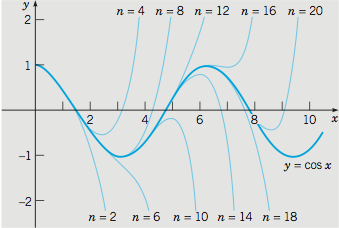
\includegraphics[scale=1]{L18besselorder0}
		\caption{Polynomial Approximation of cosine x (from B\&P)}
	\end{figure}
% end lecture 18 (2 November)

% start lecture 19 (7 November)
\section{Lecture 19: Bessel Equations continued, Laplace Transforms}
\subsection{Bessel Equations of Order 0 continued}
	By Frobenius' Theorem with repeated roots $r_1 = r_2$, our second solution has the form
		$$ y_2 (x) = y_1 (x) \ln (x) + \sumseriesone b_n (r_1) x^n $$
	for $x > 0$ where $b_n (r_1) = b_n (0) = a'_n (0)$. However,
		$$ a_n (r) = - \frac{a_{n-2} (r)}{(r+n)^2} $$
	and note that last time we considered the case where $r=0$. For general $r$,
		$$ a_2 = - \frac{a_0}{(r+2)^2} $$
		$$ a_{2n} (r) = \frac{(-1)^n a_0}{(r+2)^2 (r+4)^2 \cdots (r+2n)^2} $$

	To find $a'_{2n} (r)$, note that if
		$$ f(x) = (x - \alpha_1)^{\beta_1} (x - \alpha_2)^{\beta_2} \cdots (x - \alpha_n)^{\beta_n} $$
	then, if $x \neq \alpha_1$, we have
		$$ \frac{f'(x)}{f(x)} = \frac{\beta_1}{x - \alpha_1} + \frac{\beta_2}{x - \alpha_2} + \cdots + \frac{\beta_n}{x - \alpha_n}. $$
	Now
		$$ \frac{a'_{2n} (r)}{a_{2n} (r)} = - 2 \left(\frac{1}{r+2} + \frac{1}{r + 4} + \cdots + \frac{1}{r + 2n} \right) $$
	and setting $r = 0$:
		$$ \frac{a'_{2n} (0)}{a_{2n} (0)} = -2 \left( \frac{1}{2} + \frac{1}{4} + \cdots + \frac{1}{2n} \right) $$
		$$ a'_{2n} (0) = - \underbrace{\left(1 + \frac{1}{2} + \frac{1}{3} + \cdots + \frac{1}{n} \right)}_{H_n} a_{2n} (0) $$
		$$ a'_{2n} (0) = - H_n a_{2n} (0) $$
		$$ b_{2n} (0) = a'_{2n} (0) = - \frac{H_n (-1)^n a_0}{2^{2n} (n!)^2} \text{ for } n = 1, 2, 3, \ldots $$

	Meanwhile, what is $b_{2n+1} (0)$? We have $a_1(r)$ and so $a_{2n+1}(r) = 0 = a'_{2n+1}(r) = b_{2n+1} (0)$.

	Then we have our second solution:
		$$ \boxed{y_2 (x) = J_0 (x) \ln (x) + \sumseriesone \frac{(-1)^{n+1} H_n x^{2n}}{2^{2n} (n!)^2}} $$

	Any linear combination of $y_1$ and $y_2$ will also be a solution, and actually the Bessel function of the second kind of order 0, denoted $Y_0 (X)$, is taken to be
		$$ \boxed{Y_0 (x) = \frac{2}{\pi} \left[y_2 (x) + (\gamma - \ln(2)) J_0 (x) \right]} $$
	where
		$$ \gamma = \limseq (H_n - \ln(n)) \approx 0.5772\ldots $$

	Now the general solution of the \textbf{Bessel Equation of Order 0} can be written as
		$$ y(x) = c_1 J_0 (x) + c_2 Y_0 (x) $$

\subsection[Bessel Equation of Order 1/2]{Bessel Equation of Order $\frac{1}{2}$}
	Setting $\nu = \frac{1}{2}$ we have
		$$ x^2 y'' + x y' + \left(x^2 - \frac{1}{4} \right) y = 0 $$
	with the indicial equation
		$$ F(r) = r^2 - \frac{1}{4} = 0 $$
	with roots $r_1 = \frac{1}{2}$ and $r_2 = - \frac{1}{2}$. $r_1 = \frac{1}{2}$ leads to one solution, but since $r_1 - r_2 = 1$, we'll have to use the case of Frobenius' Theorem where $r_1 - r_2 = n \in \mathbb{N}$.

	Substituting $y(x) = x^r \sumseries a_n (r) x^n $ into the ODE, we eventually obtain
		$$ 0 = \left(r^2 - \frac{1}{4}\right) a_0 (r) x^r + \left[(r+1)^2 - \frac{1}{4} \right] a_1 (r) x^{r+1} + \sumseriestwo \left[ \left[ (r+n)^2 - \frac{1}{4} \right] a_n + a_{n-2} \right] x^{n + r} .$$

	Now we must define a continuous function $a_1 (r)$ such that $\left[(r+1)^2 - \frac{1}{4} \right] a_1 (r) = 0$, then we must have $a_1 (r) = 0 \; \forall r$ since $(r+1)^2 - \frac{1}{4} \neq 0$ for all but two values of $r$.

	The last term gives us the recurrence relation
		$$ \boxed{a_n (r) = \frac{- a_{n-2} (r)}{(r+n)^2 - \frac{1}{4}} \text{ for } n \geq 2} $$

	Immediately we find that $a_{2n+1} (r) = 0 \; \forall r$. For even coefficients, set $r = \frac{1}{2}$ then
		$$ a_n = \frac{- a_{n-2}}{n(n+1)} $$
	hence
		$$ a_2 = (-1) \frac{a_0}{3 \times 2} ,$$
		$$ a_4 = (-1)^2 \frac{a_0}{5 \times 4 \times 3 \times 2}, $$
	and
		$$ a_{2n} = (-1)^n \frac{a_n}{(2n+1)!}.$$

	Thus, taking $a_0 = 1$, we get a solution
		$$ \boxed{y_1 (x) = x^{-1/2} \left[\sumseries \frac{(-1)^n x^{2n}}{(2n+1)!}\right] = x^{-1/2} \sin (x)} \text{ for } x > 0 $$

	The Bessel function of order $\frac{1}{2}$ is thus defined to be
		$$ \boxed{J_{\frac{1}{2}} (x) = \left(\frac{2}{\pi}\right)^{1/2} y_1 (x) = \left( \frac{2}{\pi x} \right)^{1/2} \sin(x)} $$

	For a second solution with $r_1 - r_2 = 1$, from Frobenius' Theorem, we have
		$$ y_2 (x) = a y_1 (x) \ln (x) + x^{-1/2} \left[ 1 + \sumseriesone c_n \left(- \frac{1}{2} \right) x^n \right] $$

	Here we have $a = \lim_{r \to r_2} (r-r_2)a_N (r)$ where $N = (r_1 - r_2) = 1$ so
		$$ a = \lim_{r \to r_2} (r - r_2) a_1 (r) $$
	but from before we have $a_1 (r) = 0$, so $a = 0$, and we don't need a logarithmic term, so
		$$ y_2 (x) = x^{-1/2} \left[1 + \sumseriesone c_n (r) x^n \right] $$

	Now using the formula for $c_n (r)$ for the direction substitution into the ODE, we find
		$$ y_2 (x) = x^{-1/2} \left[ a_0 \sumseries \frac{(-1)^n x^{2n}}{(2n)!} + a_1 \sumseries \frac{(-1)^n x^{2n+1}}{(2n+1)!} \right] $$
		$$ \Rightarrow y_2 (x) = \frac{a_0}{x^{1/2}} \cos(x) + \underbrace{\frac{a_1}{x^{1/2}} \sin(x)}_{\text{multiple of } y_1 (x)} $$

	Usually we define $J_{-\frac{1}{2}} (x)$ by taking $a_0 = \left(\frac{2}{\pi}\right)^{1/2}$ and $a_1 = 0$, so
		$$ \boxed{J_{-\frac{1}{2}} (x) = \left(\frac{2}{\pi x}\right)^{1/2} \cos(x)} \text{ for } x > 0 $$


	For the Bessel Equation of Order 1, $a \neq 0$, so we will require a logarithmic term in the solution. See the textbook for this solution.

\subsection{Laplace Transforms}
	Laplace Transforms were developed by Laplace and Heaviside.

	\definition let $f: [0, \infty] \rightarrow \mathbb{R}$, then the \emph{Laplace Transform} of $f$, denoted by $\lap\{f(t)\}$ or $F(s)$, is a function of $s$ defined by
		$$ F(s) = \lap\{f(t)\} = \int_0^{\infty} e^{-st} f(t) \,dt $$

	\textbf{Remarks:}
		\begin{itemize}
			\item $s$ may be real or complex, but in this course we will only deal with cases where $s$ is real.
			\item Here,
				$$ \intzi \cdots dt = \lim_{t \to \infty} \int_0^t \cdots dt $$
			and we'll worry below about when the limit exists.
			\item We'll be interested in transforms of discontinuous functions and we'll transform entire differential equations to solve them.
		\end{itemize}

	\definition a function $f$ is said to be \emph{piecewise continuous} (or PWC) for $t \in [\alpha, \beta]$ if $[\alpha, \beta]$ can be partitioned by a finite number of points $\alpha = t_0 < t_1 < t_2 < \ldots < t_n = \beta$ such that
		\begin{enumerate}
			\item $f$ is continuous on each open interval $t \in (t_i, t_{i+1})$ and
			\item for $t \in (t_i, t_{i+1})$, $\lim_{t \to t_i} f(t)$ and $\lim_{t \to t_{i+1}} f(t)$ both exist and are finite.
		\end{enumerate}
	We say $f$ is PWC on $[\alpha, \infty)$ if $f$ is PWC on $[\alpha, \beta]$ for each $\beta \in (\alpha, \infty)$.

	\example $\tan(t)$ is not PWC because $\lim_{t \to \frac{\pi}{2}} \tan(t) = + \infty$.

	For a PWC function, jump discontinuities are allowed, but the solutions must remain bounded.

	\textbf{Remark:}
		$$ \int_{\alpha}^{\beta} f(t) \,dt = \sum_{i = 0}^{n-1} \int_{t_i}^{t_{i+1}} f(t)\,dt $$
	and the values of discontinuities are not important.

	\definition a function $f(t)$ is said to have \emph{exponential order ``a''} (or simply exponential order) if there exists constants $K,T$ such that
		$$ |f(t)| \leq K e^{aT} \; \forall t \leq T. $$

	\begin{thm}
		Suppose $f$ is PWC for $t \in [0, \infty)$ and that $f(t)$ has exponential order $a$. Then, the Laplace Transform $\lap \{f(t) \} = F(S)$ exists for $s > a$.
	\end{thm}

	\textbf{Proof:}
		$$ F(S) = \intzi e^{-st} f(t) \,dt = \int_0^m e^{-st} f(t) \, dt + \int_m^{\infty} e^{-st} f(t) \, dt $$
	The first term is finite because $f(t)$ is PWC on $[0,m]$. We need to show that the second term is finite. Assuming $m > T$,
		$$ \int_m^{\infty} e^{-st} f(t) \, dt \leq K \int_m^{\infty} e^{-st} e^{at} \, dt = K \left[\frac{e^{t(a-s)}}{a-s}\right]_m^{\infty} = \frac{-k e^{m(a-s)}}{a-s} < \infty $$
	so the interval converges, and thus is finite. $\square$

	Laplace Transforms do not exist for all functions e.g. for $e^{t^2}$ as this is not of exponential order, or for $\frac{1}{t}$, which is not PWC.

\subsubsection{Laplace Transforms of some useful functions}

	$f(t) = e^{at}$ is trivially of exponential order, so $\lap\{e^{at}\}$ exists. Indeed,
		$$ \lap\{e^{at}\} = \intzi e^{-st} e^{at} \,dt = \intzi e^{(a-s)t} \, dt = \left[\frac{e^{(a-s)t}}{a-s}\right]_0^{\infty} = \frac{1}{s-a} $$
	so $\lap\{e^{at}\} = \frac{1}{s-a}$.

	As a special case, taking $a=0$, $\lap\{1\} = \frac{1}{s}$ for $s > 0$. Also, $t < 1 + t < e^t$ for $t > 0$, so $t$ is of exponential order $1$, so
		$$ \lap\{t\} = \intzi e^{-st} t \, dt = \left[ \frac{t e^{-st}}{-s} \right]_{t=0}^{\infty} - \intzi \frac{e^{-st}}{-s}\,dt $$

	Noting that, for $k > 0$,
		$$ \lim_{t \to \infty} t e^{-kt} = \lim_{t \to \infty} \frac{t}{e^{kt}} = \lim_{t \to \infty} \frac{1}{k e^{kt}} = 0 $$
	so
		$$ \lap\{t\} = \frac{1}{s} \intzi e^{-st}\,dt = \frac{1}{s} \lap\{1\} = \left(\frac{1}{s}\right) \left(\frac{1}{s}\right) = \frac{1}{s^2} $$

	For $\lap \{\cos(\omega t) \}$ since $|\cos(\omega t)| \leq 1$, this is clearly of exponential order $0$. Thus,
		\begin{align*}
			F(s) &= \intzi e^{-st} \cos(\omega t)\,dt \\
				&= \left[- \frac{1}{s} e^{st} \cos(\omega t)\right]_{t=0}^{\infty} - \frac{\omega}{s} \intzi e^{-st} \sin(\omega t)\,dt \\
				&= \frac{1}{s} - \frac{\omega}{s} \left[ \left[ - \frac{1}{s} e^{-st} \sin(\omega t)\right]_0^{\infty} + \frac{w}{s} \intzi e^{-st} \cos(\omega t)\,dt \right] \\
			F(s) &= \frac{1}{s} - \frac{\omega^2}{s^2} F(s) \\
			F(s) &= \frac{s}{s^2 + \omega^2}
		\end{align*}
	Similarly, $\lap\{\sin(\omega t)\} = \frac{\omega}{s^2 + \omega^2}$.

	There will be a table of Laplace Transforms on the final exam.

\subsubsection{Linearity of Laplace Transforms}
	It is important to realize that Laplace Transforms are linear operators in the sense that
		\begin{align*}
			\lap\{ \alpha f(t) + \beta g(t)\} &= \intzi e^{-st} (\alpha f(t) + \beta g(t))\,dt \\
				&= \alpha \intzi e^{-st} f(t) \,dt + \beta \intzi e^{-st} g(t) \,dt \\
				&= \alpha \lap\{f(t)\} + \beta \lap\{g(t)\}
		\end{align*}
% end lecture 19 (7 November)

% start lecture 20 (9 November)
\section{Lecture 20: Solving ODEs with Laplace Transforms}
\subsection{Some theorems}
	\begin{thm}
		If $f$ is a PWC (or simply continuous) function and of exponential order, then
			$$ \lim_{s \to \infty} F(s) = 0. $$
	\end{thm}

	\textbf{Remark:} thus, $F(s) = 1$ and $F(s) = \frac{s}{s+1}$ are not Laplace Transforms of PWC functions of exponential order.

	\textbf{Proof:}
		$$ F(s) = \lim_0^m e^{-st} f(t) \,dt + \int_m^{\infty} e^{-st} f(t) \,dt $$
	For the first term:
		$$ \int_0^m e^{-st} f(t) \,dt \leq \max_{t \in [0,m]} |f(t)| \int_0^m e^{-st} \,dt = \left[\frac{e^{-st}}{-s} \right]_{t=0}^m \to 0 \text{ as } s \to s \to + \infty .$$
	Similarly, but using the fact that $f$ is of exponential order:
		$$ \int_m^{\infty} e^{-st} f(t) \,dt \leq k \int_m^{\infty} e^{-st} e^{at} \,dt \leq k \left[ \frac{e^{t(m-s)}}{s-a}\right]_m^{\infty} \to 0 \text{ as } s \to + \infty . $$
	$\square$

	\begin{thm}
		\textbf{The First Translation Theorem:} if $\lapft = F(s)$, then
			$$ \lap\{e^{at} f(t)\} = F(s-a). $$
	\end{thm}
	\textbf{Proof:}
		$$ \lap\{e^{at} f(t)\} = \intzi e^{-st} e^{at} f(t) \, dt = \intzi e^{-(s-a)t} f(t) \,dt $$
	But if $F(s) = \intzi e^{-st} f(t) \,dt$, then
		$$ F(s-a) = \intzi e^{-(s-a)t} f(t) \,dt . \; \; \square$$

	Therefore, the Laplace Transform of $e^{at} f(t)$ is the Laplace Transform of $f(t)$ with $s$ replaced by $s-a$. It's sometimes useful in examples to show this explicitly.

	\example
		$$ \lap\{e^{at} \cos(\omega t)\} = \lap\{\cos(\omega t)\} \Big|_{s \to s-a} = \frac{s}{s^2 + \omega^2} \Big|_{s \to s-a} = \frac{s-a}{(s-a)^2 + \omega^2} $$

\subsubsection{Transforms of Derivatives}
	\begin{thm}
		Suppose that $f, f', f'', \ldots, f^{(n-1)}$ are continuous on $[0,\infty)$ and $f^{(n)}$ is PWC on $[0,\infty)$ and all of exponential order $a$. Then, $\lap\{f^{(n)} (t)\}$ exists for $s > a$ and
			\begin{align*}
				\lap\{f^{(n)} (t)\} &= s^n \lapft - s^{n-1} f(0) - s^{n-2} f'(0) - \ldots - s f^{(n-2)} (0) - f^{(n-1)} (0) \\
					&= s^n \lapft - \sum_{k=0}^{n-1} s^{n-1-k} f^{(k)} (0).
			\end{align*}
	\end{thm}

	\textbf{``Proof'':} let's first assume that $f$ and all its derivatives are continuous. Then,
		\begin{align*}
			\lap\{f'(t)\} &= \intzi e^{-st} f'(t)\,dt \\
				&= \left[e^{-st} f(t)\right]_0^{\infty} - \intzi -s e^{-st} f(t) \,dt \\
				&= -f(0) + s \intzi e^{-st} f(t) \,dt \\
				&= -f(0) + s \lapft \\
				&= s \lapft - f(0) \\
			\lap\{f''(t)\} &= s \lap\{f'(t)\} - f'(0) \\
				&= s \left[s \lapft - f(0)\right] - f'(0) \\
				&= s^2 \lapft - sf(0) - f'(0)
		\end{align*}
	Now to prove the general result, we must use induction. In the case where $f'(t)$ has discontinuities at $t_0, \ldots, t_n \in [0,A]$, derive the result for $\lap\{f'(t)\}$ as above, noting that
		\begin{align*}
			\int_0^A e^{-st} f(t) \,dt &= \sum_{i=0}^{n-1} \int_{t_i}^{t_{i+1}} e^{-st} f'(t) \,dt \\
				&= \sum_{i=0}^{n-1} \left[e^{-st} f(t)\right]_{t_i}^{t_{i+1}} + s \sum_{i=0}^{n-1} \int_{t_i}^{t_{i+1}} e^{-st} f(t) \, dt
		\end{align*}
	and as $f(t)$ is continuous,
		$$ \int_0^A e^{-st} f(t) \,dt = e^{-s t_n} f(t_n) - f(0) + s \int_{t_i}^{t_{i+1}} e^{-st} f(t) \, dt .$$
	Now take the limit as $A \to \infty$ to get our original result. $\square$

\subsection{Solving constant-coefficient linear ODEs with Laplace Transforms}
	Let $L[y] = \sum_{k=0}^n a_k y^{(k)}$ for constants $a_0, a_1, \ldots, a_n$ with $a_n \neq 0$. Solve $L[y] = g(t)$ subject to the initial conditions $y(0) = y_0$, $y'(0) = y_1$, $y''(0) = y_2$, $\ldots$, $y^{(n-1)} (0) = y_{n-1}$. We will solve this IVP by taking the Laplace transform of the entire differential equation.
		\begin{align*}
			g(t) &= L[y] (t) \\
			\Rightarrow \lap\{g(t)\} &= \lap\{L[y](t)\} \\
				&= \lap\{ \sum_{k=0}^n a_k y^{(k)} (t)\} \\
				&= \sum_{k=0}^n a_k \lap\{y^{(k)} (t)\} \text{ using the linearity of } \lap.
		\end{align*}
	Let $Y(s) = \lap\{y(t)\}$ and $G(s) = \lap\{g(t)\}$. Then,
		\begin{align*}
			G(s) &= \sum_{k=0}^n a_k \left[s^k \lap\{y(t)\} - \sum_{j=0}^{k-1} s^{k-1-j} y^{(j)} (0) \right] \\
			\Rightarrow G(s) &= \underbrace{\left[\sum_{k=0}^n a_k s^k \right]}_{P(s)} Y(s) - \underbrace{\sum_{k=0}^n a_k \left[\sum_{j=0}^{n-1} s^{k-1-j} y^{(j)} (0) \right]}_{Q(s)} \\
			G(s) &= P(s) Y(s) - Q(s) \\
			\Rightarrow Y(s) &= \frac{Q(s) + G(s)}{P(s)}
		\end{align*}
	Notice that $P(s)$ is the characteristic function which appears as a function of $r$ in the auxiliary equation for an $n$th order ODE. $Q(s)$ is a known polynomial in $s$ of degree $n-1$ and dependent on the initial conditions. $G(s)$ is the Laplace transform of $g(t)$, and so $G(s) = 0$ for a homogeneous problem.

\subsubsection{The inverse Laplace transform definition}
	Now we have a formula for $Y(s) = \lap\{y(t)\}$, so we would like to invert the transform and claim that $y(t) = \lapi\{Y(s)\}$. This inversion can be done in two ways:
		\begin{enumerate}
			\item using complex analysis and the Branwich integral formula:
				$$ f(t) = \lapi\{F(s)\} = \frac{1}{2\pi i} \int_{a - i \infty}^{a + i \infty} F(s) e^{st} \,ds $$
			\item or using a table of Laplace transforms from right-to-left instead of left-to-right.
		\end{enumerate}
	The latter method is obviously preferred. Note that the Bronwich formula uniquely defines the inverse, which also implies that two continuous functions $f_1 (t)$ and $f_2(t)$ (which do not agree everywhere) must have two different Laplace transforms, i.e.
		$$ \lap\{f_1(t)\} = \lap\{f_2 (t)\} \Leftrightarrow f_1 (t) = f_2 (t) \; \forall t \geq 0 $$
	provided $f_1, f_2$ are continuous. For PWC functions $f_1, f_2$, we have the above condition if and only if both functions have the same discontinuity points $t_i$ and, for all $i$, $f_1 (t) = f_2 (t) \; \forall t \in (t_i, t_{i+1})$. However, they do not have to agree at the discrete points $t_i$.

\subsubsection{Linearity of the inverse Laplace transform}

	It is useful to note that the inverse Laplace transform is also linear, following from the linearity of the function itself.

	\example
		$$ F(S) = \frac{2s + 1}{s^2 + 4} = 2 \left(\frac{s}{s^2 + 4}\right) + \frac{1}{2} \left(\frac{2}{s^2 + 4}\right) $$
		$$ f(t) = \lapi\{F(s)\} = 2 \lapi \left\{\frac{s}{s^2+4} \right\} + \frac{1}{2} \lapi \left\{ \frac{2}{s^2+4} \right\} $$
		$$ \Rightarrow f(t) = 2 \cos(2t) + \frac{1}{2} \sin(2t) $$

	\example
		$$ F(s) = \frac{2s+1}{s^2 + 2s + 2} = \frac{2s+1}{(s+1)^2 + 1} $$
		$$ \Rightarrow F(s) = 2 \left[\frac{s+1}{(s+1)^2 + 1}\right] - 1 \left[\frac{1}{(s+1)^2 + 1}\right] $$
	Notice that
		$$ \frac{s+1}{(s+1)^2 + 1} = \left.\frac{s}{s^2 + 1}\right|_{s \to s+1} $$
		$$ \Rightarrow \lapi \left\{ \frac{s+1}{(s+1)^2 + 1} \right\} = e^{-t} \cos(t) $$
		$$ \lapi \left\{ \frac{1}{(s+1)^2 + 1} \right\} = e^{-t} \sin(t) $$
		$$ f(t) = \lapi \{F(s)\} = 2 e^{-t} \cos(t) - e^{-t} \sin(t) $$

	We will see many examples where $F(s) = \frac{A(s)}{B(s)}$ where $A,B$ are polynomials and $B$ factorizes, necessitating the use of partial fractions.
% end lecture 20 (9 November)

% start lecture 21 (14 November)
\section{Lecture 21: Laplace Transforms with Discontinuous Functions}
\subsection{Inverse Laplace Transforms with partial fractions}
\subsubsection{Example 1}
		$$ y'' - ey' + 2y = e^{-4t} $$
		$$ y(0) = 1, y'(0) = 5 $$
	\emph{Note}: to apply Laplace transforms, we require that the initial conditions be specified at $t=0$.

		\begin{align*}
			\Rightarrow \lap\{y''\} - e \lap\{y'\} + 2 \lap\{y\} &= \lap\{e^{-4t}\} \\
			[s^2 Y(s) - sy(0) - y'(0)] - 3 [sY(s) - y(0)] + 2Y(s) &= \frac{1}{s+4} \\
			(s^2 - 3s + 2)Y(s) - s - 5 + 3 &= \frac{1}{s+4} \\
			(s^2 - 3s + 2) Y(s) &= \frac{1}{s+4} + s + 2 \\
			(s-1)(s-2)Y(s) &= \frac{1}{s+4} + s + 2
		\end{align*}

		\[
			\boxed{Y(s) = \frac{1}{(s-1)(s-2)(s+4)} + \frac{s+2}{(s-1)(s-2)}}
			\tag{$\star$}
			\label{eq:partial1}
		\]

	We cannot directly inverse Laplace transform \eqref{eq:partial1}. We must use \emph{partial fractions} to rewrite $Y(s)$ as a larger sum of simpler terms.
		$$ \frac{s+2}{(s-1)(s-2)} = \frac{A}{s-1} + \frac{B}{s-2} $$
	We can find $A,B$ at least three different ways:
		\begin{enumerate}
			\item First, write
				$$ s+2 = A(s-2) + B(s-1) $$
				then, choose convenient values of $s$, since the equation holds $\forall s$. Taking $s=1$, $3 = -A \Rightarrow A = -3$, and taking $s=2$, $B=4$.
			\item Alternatively, equate the coefficients of the polynomials in the equality:
				\begin{align*}
					s^0 &\Rightarrow 2 = -2 A - B \\
					s^1 &\Rightarrow 4 = B
				\end{align*}
			\item Use the ``cover-up'' method. To find $A$ for $\frac{A}{s-1}$, take $\frac{s+2}{(s-1)(s-2)}$ and cover-up the $s-1$ term, setting $s=1$. Then, to find $B$, cover up the $s-2$ term and set $s=2$.
		\end{enumerate}
	Thus,
		$$ \frac{s+2}{(s-1)(s-2)} = \frac{-3}{s-1} + \frac{4}{s-2}. $$
	Now,
		$$ \frac{1}{(s-1)(s-2)(s+4)} = \frac{A}{s-1} + \frac{B}{s-2} + \frac{C}{s+4} $$
	and using any of the above methods, we find
		$$ A = - \frac{1}{5} \text{ and } B = \frac{1}{6} \text{ and } C = \frac{1}{30} . $$
	Thus we have
		\begin{align*}
			Y(s) &= \left( \frac{-3}{s-1} + \frac{4}{s-2}\right) + \left(\frac{-\frac{1}{5}}{s-1} + \frac{\frac{1}{6}}{s-2} + \frac{\frac{1}{30}}{s+4}\right) \\
			&= - \frac{16}{5} \left(\frac{1}{s-1}\right) + \frac{25}{6} \left(\frac{1}{s-2}\right) + \frac{1}{30} \left(\frac{1}{s+4}\right) \\
			\Rightarrow y(t) &= \lapi\{\ldots\} \\
			&= - \frac{16}{5} \lapi \left\{\frac{1}{s-1}\right\} + \frac{25}{6} \lapi \left\{\frac{1}{s-2}\right\} + \frac{1}{30} \lapi \left\{\frac{1}{s+4}\right\}
		\end{align*}

	Remember that $\lap\{e^{-at}\} = \frac{1}{s-a}$ so $e^{at} = \lapi\{\frac{1}{s-a}\}$ hence
		$$ \boxed{y(t) = \frac{16}{5} e^t + \frac{25}{6} e^{2t} + \frac{1}{30} e^{-4t} } $$

\subsubsection{Example 2}
		$$ y' + y = \sin(t) \text{ with } y(0) = 1 $$
		\begin{align*}
			\lap\{y'\} + \lap\{y\} &= \lap\{\sin(t)\} \\
			sY(s) - y(0) + Y(s) &= \frac{1}{s^2 + 1} \\
			(1 + s)Y(s) - 1 &= \frac{1}{s^2 + 1} \\
			Y(s) &= \frac{1}{s+1} + \frac{1}{(s^2 + 1)(s+1)}
		\end{align*}
		$$ \frac{1}{s^2 + 1} = \frac{A}{s+1} + \frac{Bs+C}{s^2 + 1} $$

	Skipping the partial fraction calculation, we find that $A = C = \frac{1}{2}$ and $B = - \frac{1}{2}$.
		\begin{align*}
			Y(s) &= \frac{1}{s+1} + \frac{\frac{1}{2}}{s+1} + \frac{-\frac{1}{2} s + \frac{1}{2}}{s^2 + 1} \\
				&= \frac{3}{2} \left(\frac{1}{s+1}\right) - \frac{1}{2}\left(\frac{s}{s^2 + 1}\right) + \frac{1}{2} \left(\frac{1}{s^2 + 1}\right) \\
			y(t) &= \lapi\{\ldots\} \\
				&= \frac{3}{2} e^{-t} - \frac{1}{2} \cos(t) + \frac{1}{2} \sin(t)
		\end{align*}

\subsection{The Heaviside Function}
	Laplace transforms allow us to solve linear constant-coefficient non-homogeneous IVPs all in one go, but their real power is dealing with discontinuities.

	\definition the \emph{unit step function} or {Heaviside function} $U(t-a)$ or $U_a (t)$ is defined by
		$$ U(t-a) = \left\{
				\begin{array}{cc}
					0 & \text{ when } t < a \\
					1 & \text{ when } t > a
				\end{array}
			\right.
		$$
	Such functions are useful in applications such as engineering where there is a switch. Heaviside functions are often combined with each other or other functions, e.g. $f(t) = U(t-1) - U(t-2)$ or $f(t) = U(t - \pi) \sin(t - \pi)$. The Heaviside function is also PWC and of exponential order, so it has a Laplace transform.

\subsection{The Second Translation Theorem}
	\begin{thm}
		\textbf{Second Translation Theorem:} if $F(s) = \lapft$ and $a > 0$, then
			$$ \lap\{f(t-a) U(t-a)\} = e^{-as} F(s) $$
		or
			$$ \lap\{g(t) U(t-a)\} = e^{-as} \lap\{g(t+a)\} \text{ with } g(t+a) = f(t) $$
	\end{thm}

	\textbf{Proof:}
		\begin{align*}
			\lap\{f(t-a) U(t-a)\} &= \underbrace{\int_0^a e^{-st} f(t-a) \underbrace{U(t-a)}_{ =0 \; \forall t < a} \,dt}_{= 0} + \int_a^{\infty} e^{-st} f(t-a) \underbrace{U(t-a)}_{= 1 \; \forall t \geq a} \,dt \\
				&= \int_{t=a}^{\infty} e^{-st} f(t-a) \,dt
		\end{align*}
	Letting $x = t-a$:
		\begin{align*}
			\Rightarrow &= \int_{x=0}^{\infty} e^{-s(a+x)} f(x) \,dx \\
				&= e^{-sa} \intzi e^{-sx} f(x) \,dx \\
				&= e^{-sa} F(s) \; \; \square
		\end{align*}

	\begin{cor}
		\[
			\lap\{ U(t-a) \} = \lap\{ 1 \times U(t-a) \} = \frac{e^{-as}}{s}
		\]
	\end{cor}

\subsubsection{Example}
		\[
			y' + y = f(t)) = \left\{
				\begin{array}{cc}
					0 & 0 \leq t < \pi \\
					3 \cos (t) & t \geq \pi
				\end{array}
			\right.
		\]
	Initial condition: $y(0) = 2$.
		$$ y' + y = 3 \cos (t) U(t-\pi) = 3 \cos((t-\pi) + \pi) U(t-\pi) $$
	Now taking the Laplace transform, and using the Second Translation Theorem and the $\cos(t + \pi) = - \cos(t)$ identity:
		\begin{align*}
			\lap\{ 3 \cos((t-\pi) + \pi) U(t-\pi) \} &= e^{-\pi s} \lap\{3 \cos(t + \pi)\} \\
				&= - 3 e^{-\pi s} \lap\{\cos(t)\} \\
				&= -3 e^{-\pi s} \frac{s}{s^2 + 1}
		\end{align*}
		\begin{align*}
			-3 e^{-\pi s} \frac{s}{s^2 + 1} &= \lap\{y' + y\} \\
				&= sY(s) - y(0) + Y(s) \\
				&= (s+1)Y(s) - 2 \\
			Y(s) &= \frac{2}{s+1} - \frac{3 e^{-\pi s} s}{(s+1)(s^2 + 1)} \\
				&= \ldots \text{ ( skipping partial fractions computation)} \\
			Y(s) &= \frac{2}{s+1} + 3 e^{-\pi s} \left[\frac{1}{2} \left(\frac{1}{s+1} \right) - \frac{1}{2} \left(\frac{s}{s^2 + 1}\right) - \frac{1}{2} \left(\frac{1}{s^2+1}\right) \right] \\
			y(t) &= 2 e^{-t} + \frac{3}{2} U(t-\pi) \left[e^{-(t - \pi)} - \cos(t - \pi) - \sin(t - \pi)\right]
		\end{align*}
% end lecture 21 (14 November)

% start lecture 22 (16 November)
% notes by Jess
\section{Lecture 22: Laplace Transforms of Delta Functions}
\subsection{The Dirac Delta Function}
	The modern definition of $\delta (t - t_0)$ is a distribution via its action. It is not a function in the usual sense. It has a property that, for any $a < t_0 < b$,
		$$ \int_a^b f(t) \delta (t - t_0) \,dt = 0. $$
	It picks out the value of $f$ at the point $t_0$ if you integrate across $t_0$, so
		$$ \int_a^b f(t) \delta (t - t_0) \, dt = \left\{
			\begin{array}{cc}
				0 & s < t_0 \\
				f(t_0) & s > t_0
			\end{array}
			\right. .
		$$
	In particular, if we take $f(t) = 1$, then
		$$ \int_a^b f(t) \delta (t - t_0) \, dt = \left\{
			\begin{array}{cc}
				0 & s < t_0 \\
				1 & s > t_0
			\end{array}
			\right. = U(s - t_0).
		$$
	\textbf{In some sense, the $\delta$-function is the derivative of the Heaviside function.} The Dirac delta function can also be thought of using limits: let
		$$ \delta_a (t-t_0) = \left\{
			\begin{array}{cc}
				0 & t < t_0 - a \\
				\frac{1}{2a} & t \in [t_0 - a, t_0 + a] \\
				0 & t > t_0 + a
			\end{array}
			\right.
		$$
	and notice that
		$$ \int_{-\infty}^{\infty} \delta_a (t-t_0) \,dt = \frac{1}{2a} [(t_0 + a) - (t_0 - a)] = 1 $$
	Now consider
		$$ \delta (t - t_0) = \lim_{t \to 0} \delta_a (t-t_0). $$
	If $b < t_0 < c$, then for all $a$, $b < t_0 - a < t_0 < t_0 + a < c$ so
		$$ \lim_{a \to 0} \int_b^c \delta_a (t-t_0) f(t) \,dt = \lim_{a \to 0} \frac{1}{2a} \int_{t_0 = -a}^{t_0 = a} f(t) \,dt $$
	but by the integral mean value theorem, there exists a point $t(a)$ such that $t_0 - a < t(a) < t_0 + a$ and
		$$ \int_{t_0 = -a}^{t_0 = a} f(t) \,dt = f(t(a)) = 2a .$$
	Thus,
		$$ \lim_{a \to 0} \int_b^c \delta_a (t-t_0) f(t) \,dt = \lim_{a \to 0} \frac{1}{sa} [2 a f(t(a))] = \lim_{a \to 0} f(t(a)) = f (\lim_{a \to 0} t(a)) = f(t_0) $$
	but $t _0 - a < t(a) < t_0 + a$, so $\lim_{a \to 0} t(a) = t_0$. Now, provided $f$ is continuous at $t_0$, the above holds.

\subsection{Solving ODEs with the Delta Function}
	To solve differential equations with delta functions, we will use Laplace transforms.

	\begin{thm}
		For $t_0 > 0$, $\lap\{\delta (t-t_0)\} = e^{-st_0}$.
	\end{thm}

	By convention, $\lap\{\delta(t-0)\} = \lap\{\delta(t)\} = 1$. To see this, notice
		$$ \lap\{\delta(t-t_0)\} = \intzi e^{-st} \delta(t-t_0) \, dt = e^{-st_0} $$
	or, using the $\delta_a (t-t_0)$ constant method,
		\begin{align*}
			\delta_a (t-t_0) &= \frac{1}{2a} [U(t-(t_0 - a)) - U(t - (t_0 + a))] \\
			\lap\{\delta_a (t-t_0)\} = \frac{1}{2a} \left[\frac{e^{-s(t_0 -a)}}{s} -\frac{e^{-s(t_0 + a)}}{s} \right] \\
				&= e^{-st_0} \left[\frac{e^{as} - e^{-as}}{2as}\right] \\
			\lim_{a \to 0} \lap\{\delta_a (t-t_0)\} &= e^{-st_0} \lim_{a \to 0} \left[\frac{e^{as} - e^{-as}}{2as}\right] \\
				&= e^{-s t_0} \text{ (using L'Hopital's rule)} .
		\end{align*}
	Now, provided that
		$$ \lap\{\lim_{a \to 0} \delta_a (t-t_0)\} = \lim_{a \to 0} \lap\{\delta_a (t-t_0)\} $$
	we are done.
\subsubsection{An example}
		\[
			y'' + y' + y = \delta(t - 1) + U(t-2) e^{-(t-2)}
		\]
	with $y(0) = 0$ and $y'(0) = 1$.

		$$ \lap\{ U(t-2) e^{-(t-2)} \} = \frac{e^{-2s}}{s+1} $$
		$$ \lap\{ \delta(t - 1) \} = e^{-s} $$
		$$ \lap\{ y'' + y' + y \} = s^2 Y(s) - sy(0) - y'(0) + s Y(s) - y(0) + Y(s) = (s^2 + s + 1) Y(s) - 1 $$
		$$ (s^2 + s + 1) Y(s) - 1 = e^{-s} + \frac{e^{-2s}}{s+1} $$
	Notice that $(s^2 + s + 1) = \left(s + \frac{1}{2}\right)^2 + \frac{3}{4}$, so
		$$ Y(s) = \frac{1}{\left(s + \frac{1}{2}\right)^2 + \frac{3}{4}} \left[1 + e^{-s} + \frac{e^{-2s}}{s+1} \right] $$
	Recall $\lap\{e^{-bt} f(t)\} = F(s + b)$ so $\lap\{e^{-bt} \sin(at)\} = \frac{a}{(s+b)^2 + a^2}$ so
		\begin{align*}
			\lapi \left\{\frac{1}{\left(s + \frac{1}{2}\right)^2 + \frac{3}{4}} \right\} &= \frac{2}{\sqrt{3}} \; \lapi \left\{\frac{\frac{\sqrt{3}}{2}}{\left(s + \frac{1}{2}\right)^2 + \frac{3}{4}} \right\} \\
				&= \frac{2}{\sqrt{3}} e^{- \frac{1}{2} t} \sin \left(\frac{\sqrt{3}}{2} t \right)
		\end{align*}
	So
		$$ \boxed{y(t) = \frac{2}{\sqrt{3}} e^{- \frac{1}{2} t} \sin \left(\frac{\sqrt{3}}{2} t \right) + \lapi \left\{ \frac{1}{\left(s + \frac{1}{2}\right)^2 + \frac{3}{4}} \left[e^{-s} + \frac{e^{-2s}}{s+1}\right] \right\}} $$
	and recall $\lapi \{e^{-as} F(s)\} = U(t-a) f(t-a)$ so
		$$ \lapi \left\{ \frac{1}{\left(s + \frac{1}{2}\right)^2 + \frac{3}{4}} \left[e^{-s}\right] \right\} = U(t-1) \frac{2}{\sqrt{3}} e^{-\frac{1}{2} (t-1)} \sin \left(\frac{\sqrt{3}}{2} (t-1)\right) $$
		$$ \boxed{y(t) = \frac{2}{\sqrt{3}} e^{- \frac{1}{2} t} \sin \left(\frac{\sqrt{3}}{2} t \right) + U(t-1) \frac{2}{\sqrt{3}} e^{-\frac{1}{2} (t-1)} \sin \left(\frac{\sqrt{3}}{2} (t-1)\right) + \lapi \left\{ \frac{e^{-2s}}{(s+1)(s^2+s+1)} \right\}} $$
	Again, skipping the partial fraction computation,
		$$ \lapi \left\{ \frac{e^{-2s}}{(s+1)(s^2+s+1)} \right\} = U(t-2) \left[ e^{-(t-2)} -  e^{-\frac{1}{2} (t-2)} \cos \left( \frac{\sqrt{3}}{2} (t-2)\right) + \frac{1}{\sqrt{3}}  \sin \left(\frac{\sqrt{3}}{2} (t-2) \right) \right]$$

	% now technically Lecture 23
		\begin{align*}
			y(t) = \frac{2}{\sqrt{3}} e^{- \frac{1}{2} t} \sin \left(\frac{\sqrt{3}}{2} t \right) &+ U(t-1) \frac{2}{\sqrt{3}} e^{-\frac{1}{2} (t-1)} \sin \left(\frac{\sqrt{3}}{2} (t-1)\right) \\
			&+ U(t-2) \left[ e^{-(t-2)} -  e^{-\frac{1}{2} (t-2)} \cos \left( \frac{\sqrt{3}}{2} (t-2)\right) + \frac{1}{\sqrt{3}}  \sin \left(\frac{\sqrt{3}}{2} (t-2) \right) \right]
		\end{align*}
	We can differentiate the right-hand side for $t < 1$, $t \in (0, 2)$, and $t > 2$ - doing so, we find that $y''(t)$ is discontinuous at $t=2$. As we discussed before, this is because of the Heaviside function $U(t-2)$. However, at $t=1$, we find that $y'(t)$ is discontinuous. To see why this might be, consider:
		\begin{align*}
			\lim_{\epsilon \to 0} \int_{1 - \epsilon}^{1 + \epsilon} \delta (t-1)\,dt &= 1 \\
				&= \lim_{\epsilon \to 0} \left(\int_{1 - \epsilon}^{1 + \epsilon} \delta (t-1) + U(t-2) e^{-(t-2)} \,dt \right) \\
				&= \lim_{\epsilon \to 0} \int_{1 - \epsilon}^{1 + \epsilon} y'' + y' + y \,dt
		\end{align*}
	This can only hold if
		$$ \lim_{\epsilon \to 0} \int_{1 - \epsilon}^{1 + \epsilon} y' (t) \, dt = 1 $$
	and
		$$ \lim_{\epsilon \to 0} \int_{1 - \epsilon}^{1 + \epsilon} y'(t) \,dt = \lim_{\epsilon \to 0} \int_{1 - \epsilon}^{1 + \epsilon} y(t)\,dt = \lim_{\epsilon \to 0} [y'(1 + \epsilon) - y'(1 - \epsilon)] = 1 $$
	So just from the $\delta$-function in the ODE, we see that there must be a discontinuity in the second-highest derivative.

% end lecture 22 (16 November)

% start lecture 23 (21 November)
\section{Lecture 23: Convolutions and More Laplace Transforms}
\subsection{Convolutions}
\subsubsection{Definition of the convolution}
	\definition if two functions $f,g$ are PWC on $[0, \infty)$, then the \emph{convolution} of $f,g$ (denoted by $f * g$) is defined by
		$$ (f*g) (t) := \int_0^t f(\tau) g (t-\tau) \,d\tau $$

	Not many people use convolutions because their use tends to require lots of integration by parts. Also, it's easy to confuse $t$'s and $\tau$'s.

\subsubsection{The convolution theorem}
	\begin{thm}
		\textbf{Convolution Theorem:} if $f,g$ are PWC on $[0,\infty)$ and of exponential order, then
			$$ \lap\{(f*g)(t)\} = \lapft \lap\{g(t)\} = F(s) G(s) $$
		and hence
			$$ \lapi \{F(s)G(s)\} = (f * g)(t).$$
	\end{thm}

	\textbf{Proof:}
		\begin{align*}
			\lap\{(f*g)(t)\} &= \int_{t=0}^{\infty} (f*g)(t) e^{-st} \,dt \\
				&= \int_{t=0}^{\infty} \int_{\tau=0}^t f(\tau) g (t-\tau) \,d\tau \; e^{-st} \,dt \\
				&= \int_{\tau=0}^{\infty} \int_{t = \tau}^{\infty} f(\tau) g(t-\tau) e^{-st} \,dt\,d\tau \\
				&= \int_{\tau=0}^{\infty} f(\tau)e^{-s\tau} \int_{t = \tau}^{\infty} g(t-\tau) e^{-s(t-\tau)}\,dt\,d\tau \\
				&\text{Letting $x = t-\tau$:} \\
			\Rightarrow &= \int_{\tau=0}^{\infty} f(\tau)e^{-s\tau} \,d\tau \int_{x=0}^{\infty} g(x) e^{-sx} \,dx \\
			&= F(s) G(s) \; \; \square
		\end{align*}
\subsubsection{Properties of convolutions}
	For constants $\alpha, \beta$ and functions $f(t), g(t), h(t)$:
	\begin{enumerate}
		\item $(f*g)(t) = (g*f)(t)$
		\item $((\alpha f + \beta g) * h)(t) = \alpha (f*h)(t) + \beta (g*h)(t)$
		\item $(0*g)(t) = 0$
		\item $(1*g)(t) = (g*1)(t) \neq g(t)$ (Beware!)
	\end{enumerate}

\subsubsection{Uses}
	Convolutions can be useful for finding Laplace transforms of some difficult functions.

	\example find $\lap\{\sqrt{t}\}$. Let $f=\sqrt{t}$ and let $x = \tau - \frac{t}{2}$. Then
		\begin{align*}
			(f*f)(t) &= \int_0^t \sqrt{\tau} \sqrt{t-\tau} \, d\tau \\
				&= \int_{-\frac{t}{2}}^{\frac{t}{2}} \sqrt{x + \frac{t}{2}} \sqrt{\frac{t}{2} - x} \,dx \\
				&= \int_{-\frac{t}{2}}^{\frac{t}{2}} \left(\frac{t^2}{4} - x^2 \right)^{\frac{1}{2}} \, dx \\
				&= \ldots \\
				&= \frac{\pi t^2}{8}
		\end{align*}
	But now
		\[
			\lap\{(f*f)(t)\} = \lap \left\{\frac{\pi t^2}{8} \right\} = \frac{\pi}{8} \times \frac{2}{s^3} = \frac{\pi}{4s^3}
		\]
	and by the convolution theorem,
		$$ \lap\{(f*f)(t)\} = F(s) F(s) $$
	so
		$$ F(s) = \sqrt{\frac{\pi}{4s^3}} = \frac{\sqrt{\pi}}{2 s^{3/2}} = \lap\{\sqrt{t}\}. $$

	The convolution theorem can also be used to avoid partial fractions, but the approach using partial fractions is generally quicker and less error-prone.

\subsection{Laplace transforms of ODEs}
	Laplace transforms are only useful for linear ODEs. We make essential use of the linearity in several places. Also, they are rarely used for non-constant coefficient equations. In particular, they should not be applied to Euler equations, as an in-class example showed - taking the Laplace transform of a Euler equation simply gives another Euler equation.

\subsubsection{Transforms of Periodic Functions}
	\definition $f(t)$ is \emph{periodic} if $f(t) = f(t + T)$ for some $T>0$ and $\forall t > 0$.

	We already have Laplace transforms of sine and cosine, but any periodic function has a Laplace transform.

	\begin{thm}
		if $f(t)$ is PWC on $[0,\infty)$ and periodic with period $T$, then
			$$ \lapft = F(s) = \frac{1}{1 - e^{-st}} \int_0^T e^{-st} f(t) \,dt $$
	\end{thm}

	\textbf{Proof:} Letting $x = t-T$:
		\begin{align*}
			F(s) &= \int_0^T e^{-st} f(t) \,dt + \int_T^{\infty} e^{-st} f(t) \,dt \\
			\Rightarrow \int_T^{\infty} e^{-st} f(t) \,dt &= \intzi e^{-s(x+T)} f(x+T) \,dx \\
				&= e^{-sT} \intzi e^{-sx} f(x) \, dx \text{ as $f$ is periodic} \\
				&= e^{-sT} F(s)
		\end{align*}
	and the result follows. $\square$

	\example the Square Wave $f(t) = \sum_{n=0}^{\infty} (-1)^n U(t-n)$. Because this is period with $T=2$, then
		\begin{align*}
			\lapft &= \frac{1}{1 - e^{-2s}} \int_0^2 e^{-st} f(t) \,dt \\
				&= \frac{1}{1 - e^{-2s}} \int_0^1 e^{-st}\,dt \\
				&= \frac{1}{1 - e^{-2s}} \left[\frac{e^{-st}}{-s}\right]_{t=0}^1 \\
				&= \frac{1}{1 - e^{-2s}} \left[\frac{e^{-s}}{-s} + \frac{1}{s} \right] \\
				&= \ldots \\
				&= \frac{1}{s(1+e^{-s})}
		\end{align*}

\subsection{End of class remarks}
	This lecture represents the final lecture of examinable material. More material follows in the three remaining lectures, but that material will not be present on the final exam, so I did not bother to take notes or type them up.
% end lecture 23 (21 November)

% all lectures following lecture 23 are not examinable

























\end{document}